\documentclass[12pt]{elsarticle}

\usepackage[margin=1in]{geometry}
\usepackage{lineno,graphicx, amsmath, esvect, amssymb, ragged2e, afterpage, placeins}
\usepackage[colorlinks]{hyperref}
\usepackage[labelformat=simple]{subcaption}
\numberwithin{equation}{section}
\numberwithin{figure}{section}
\numberwithin{table}{section}
\usepackage{cleveref}
\renewcommand\thesubfigure{(\alph{subfigure})}
\modulolinenumbers[1]
\usepackage{fancyhdr}
\pagestyle{fancy}
\fancyhf{}
\setlength{\headheight}{14pt}
\chead{\small{\textit{This is a revised preprint submitted to the \href{https://www.journals.elsevier.com/cold-regions-science-and-technology/editorial-board}{Elsevier CRST} journal and hosted by \href{https://eartharxiv.org/6v4h3/}{EarthArXiv}.}}}
\rfoot{\small\textit{\thepage}}
\lfoot{\small\textit{Majumdar et al., 2020}}
\cfoot{\small\textit{Cold Regions Science and Technology}}
%\journal{Cold Regions Science and Technology}
\fancypagestyle{pprintTitle}{%
\chead{\small{\textit{This is a revised preprint submitted to the \href{https://www.journals.elsevier.com/cold-regions-science-and-technology/editorial-board}{Elsevier CRST} journal and hosted by \href{https://eartharxiv.org/6v4h3/}{EarthArXiv}.}}}
%\renewcommand{\headrulewidth}{0.0pt}
}

\setcounter{secnumdepth}{4}

%\titleformat{\paragraph}
%{\normalfont\normalsize\it}{\theparagraph}{1em}{}
%\titlespacing*{\paragraph}
%{0pt}{3.25ex plus 1ex minus .2ex}{1.5ex plus .2ex}

%%%%%%%%%%%%%%%%%%%%%%%
%% Elsevier bibliography styles
%%%%%%%%%%%%%%%%%%%%%%%
%% To change the style, put a % in front of the second line of the current style and
%% remove the % from the second line of the style you would like to use.
%%%%%%%%%%%%%%%%%%%%%%%

%% Numbered
%\bibliographystyle{model1-num-names}

%% Numbered without titles
%\bibliographystyle{model1a-num-names}

%% Harvard
%\bibliographystyle{model2-names.bst}\biboptions{authoryear}

%% Vancouver numbered
%\usepackage{numcompress}\bibliographystyle{model3-num-names}

%% Vancouver name/year
%\usepackage{numcompress}\bibliographystyle{model4-names}\biboptions{authoryear}

%% APA style
\bibliographystyle{model5-names}\biboptions{authoryear}

%% AMA style
%\usepackage{numcompress}\bibliographystyle{model6-num-names}

%% `Elsevier LaTeX' style
%\bibliographystyle{elsarticle-num}
%%%%%%%%%%%%%%%%%%%%%%%

\tolerance=1
\emergencystretch=\maxdimen
\hyphenpenalty=10000
\hbadness=10000
\sloppy

\usepackage{scalerel}
\usepackage{tikz}
\usetikzlibrary{svg.path}

\definecolor{orcidlogocol}{HTML}{A6CE39}
\tikzset{
  orcidlogo/.pic={
    \fill[orcidlogocol] svg{M256,128c0,70.7-57.3,128-128,128C57.3,256,0,198.7,0,128C0,57.3,57.3,0,128,0C198.7,0,256,57.3,256,128z};
    \fill[white] svg{M86.3,186.2H70.9V79.1h15.4v48.4V186.2z}
                 svg{M108.9,79.1h41.6c39.6,0,57,28.3,57,53.6c0,27.5-21.5,53.6-56.8,53.6h-41.8V79.1z M124.3,172.4h24.5c34.9,0,42.9-26.5,42.9-39.7c0-21.5-13.7-39.7-43.7-39.7h-23.7V172.4z}
                 svg{M88.7,56.8c0,5.5-4.5,10.1-10.1,10.1c-5.6,0-10.1-4.6-10.1-10.1c0-5.6,4.5-10.1,10.1-10.1C84.2,46.7,88.7,51.3,88.7,56.8z};
  }
}

\newcommand\orcidicon[1]{\href{https://orcid.org/#1}{\mbox{\scalerel*{

\begin{tikzpicture}[yscale=-1,transform shape]
\pic{orcidlogo};
\end{tikzpicture}
}{|}}}}

\DeclareMathOperator{\sinc}{sinc}
\begin{document}
\linenumbers
\begin{frontmatter}
\title{\textbf{Snow Depth and Snow Water Equivalent Estimation in the Northwestern Himalayan Watershed using Spaceborne Polarimetric SAR Interferometry}}
%\tnotetext[mytitlenote]{Fully documented templates are available in the elsarticle package on \href{http://www.ctan.org/tex-archive/macros/latex/contrib/elsarticle}{CTAN}.}

%% Group authors per affiliation:
%\author{Sayantan Majumdar\fnref{myfootnote}, Praveen K. Thakur, Ling Chang, Shashi Kumar}
%\address{Faculty ITC, University of Twente}
%\fntext[myfootnote]{Since 1880.}

%% or include affiliations in footnotes:
\author[itc,iirs]{\orcidicon{0000-0002-3539-0147} Sayantan Majumdar \corref{corrauth}}
\cortext[corrauth]{Corresponding author}
\ead{ir.sayantan.majumdar@gmail.com}
\author[iirs]{\orcidicon{0000-0002-2719-7021} Praveen K. Thakur}
%\ead{praveen@iirs.gov.in}
\author[itc]{\orcidicon{0000-0001-8212-7221} Ling Chang}
%\ead{ling.chang@utwente.nl}
\author[iirs]{\newline\orcidicon{0000-0002-2442-7143} Shashi Kumar}
%\ead{shashi@iirs.gov.in}
\author[sase]{\orcidicon{0000-0003-4946-4634} Sneh Mani}
%\ead{snehmani@gmail.com}

\address[itc]{Faculty of Geo-information Science and Earth Observation (ITC), University of Twente}
\address[iirs]{Indian Institute of Remote Sensing (IIRS), ISRO}
\address[sase]{Snow and Avalanche Study Establishment (SASE), DRDO}

\begin{abstract}
\begin{linenumbers}
\small{Snow depth (SD) and Snow Water Equivalent (SWE) constitute essential physical properties of snow and find extensive usage in the hydrological modelling domain. However, the prominent impact of the hydrometeorological conditions and difficult terrain conditions inhibit accurate measurement of the SD and SWE--- an ongoing research problem in the cryosphere paradigm. In this context, spaceborne synthetic aperture radar (SAR) systems benefit from global coverage at sufficiently high spatial and temporal resolutions. Still, existing polarimetric and interferometric SAR techniques are susceptible to high volume scattering resulting from the increased snow grain sizes due to the standing (or old) snow formation driven by the temperature induced snow metamorphosis process. Hence, to model this volume decorrelation, the polarimetric SAR interferometry (Pol-InSAR) technique can be effectively applied. In this work, the standing snow depth (SSD) and its corresponding standing snow water equivalent (SSWE) are estimated using the single-baseline Pol-InSAR based hybrid Digital Elevation Model (DEM) differencing and coherence amplitude inversion model. To achieve this, six TerraSAR-X, TanDEM-X Coregistered Single look Slant range Complex (CoSSC) bistatic quad-pol acquisitions between December 2015 and January 2016 over Dhundi (situated in the Beas watershed, northwestern Himalayas, India) are used. Due to the associated problems of model parameter tuning, complex topographical conditions, and limited ground-truth measurements, appropriate sensitivity analyses have been carried out for the parameter optimisation. Furthermore, the uncertainty sources are identified by performing a summer (June 8, 2017) and wintertime (January 8, 2016) comparative analysis of the study area which quantitatively highlights the changes in the percentages of the surface and volume scatterings. Evidently, the improved model displays sufficiently high overall SSD accuracy with coefficient of determination ($R^2$) $\approx$ 0.97, Mean Absolute Error (MAE) $\approx$ 1.56 cm, and Root Mean Square Error (RMSE) $\approx$ 1.89 cm. Additionally, the respective SSWEs have been calculated by assuming a fixed snow density for each epoch wherein the overall error metrics are $R^2 \approx$ 0.78, MAE $\approx$ 4.84 mm, and RMSE $\approx$ 6.01 mm. Therefore, this research successfully demonstrates the practicability of the improved Pol-InSAR model for SD estimation over rugged terrains.}
\end{linenumbers}
\end{abstract}

\begin{keyword}
\small{Pol-InSAR, Microwave Remote Sensing, Synthetic Aperture Radar, Polarimetry, Interferometry, Snow Depth, Snow Water Equivalent, Watershed, Sensitivity Analysis}
\end{keyword}

\end{frontmatter}
\thispagestyle{fancy}
\section{Introduction}
\label{sec:Intro}

Snow depth (SD) and snow water equivalent (SWE) are two of the most important physical properties of snow and are extensively used in hydrological models that relate to snowmelt runoff and snow avalanche predictions \citep{Thakur2017}. While snow depth or snow height refers to the distance of the ground to the snow surface, SWE quantifies the amount of water present in a snowpack (layered snow formed by accumulation over time). Theoretically, SWE is defined as the product of snow depth and snow density and can be conceptualised as the amount of liquid water obtained owing to the instantaneous melting of
an entire snowpack \citep{Tedesco2015}. Obtaining accurate estimation of the SD and SWE is quite challenging depending upon the data availability, variety, and quality, parameterisation method, mathematical model selection, and the hydrometeorological conditions. Hence, it is considered to be an important research element in the cryosphere paradigm \citep{Leinss2014, Leinss2015, Leinss2016, Conde2018}.

Due to the difficulties posed by in-situ or ground based measurements of the SD and SWE in rugged terrains, remote sensing techniques coupled with adequately sampled (both in space and time domains) ground measurements are widely used to improve the quality of these estimated parameters over considerably large areas \citep{Takala2011}. Currently, LiDAR (Light Detection and Ranging) and spaceborne SAR (Synthetic Aperture Radar) are the most popular techniques used in the studies related to snow, ice and the cryosphere in general \citep{Deems2013, Leinss2014, Tedesco2015}. However, LiDAR can only be used to determine the height of the snow and cannot be used for measuring other physical properties such as snow density and snow wetness \citep{Tedesco2015, Leinss2014}. In addition, the operating cost of LiDAR is sufficiently high and is also weather dependent \citep{Deems2013}. As a result, spaceborne SAR systems benefit from substantial coverage (globally available), cloud insensitivity, all-day operability and are extensively used to measure the snow physical properties sufficiently at high spatial resolutions \citep{Moreira2013, Thakur2012}.

The applicability of SAR systems for snow cover monitoring was discussed as early as 1977 \citep{Ulaby1977} wherein the snow backscatter coefficient was measured and was thereafter modelled for various frequencies, layers, and polarisations \citep{Zuniga1979}. It was shown that only very high microwave frequencies (Ku-band or higher) exhibit a significant dependence on SD or the SWE of dry or standing (deposited) snow \citep{Yueh2009}. However, lower frequencies (X-band or below) penetrate through dry snow whereby the underneath frozen soil or ground primarily contributes to the radar backscatter signal. Whereas, in case of moist snow (the transitional stage between dry and wet snow) and wet snow, the predominant scattering occurs from the snow volume and snow surface respectively due to the presence of water. Essentially, water, with its high dielectric constant, heavily modifies the dielectric properties of snow and effectively reduces the snow penetration capacity of the radar pulses \citep{Abe1990}. The radar backscattering mechanism for a typical snow covered area can be conceptualised from Figure \ref{fig:concept}. In principle, Polarimetric SAR (PolSAR) and Interferometric SAR (InSAR) techniques utilise these received target echoes to support various microwave remote sensing applications in the cryosphere domain.

\begin{figure}[htb]
    \centering
    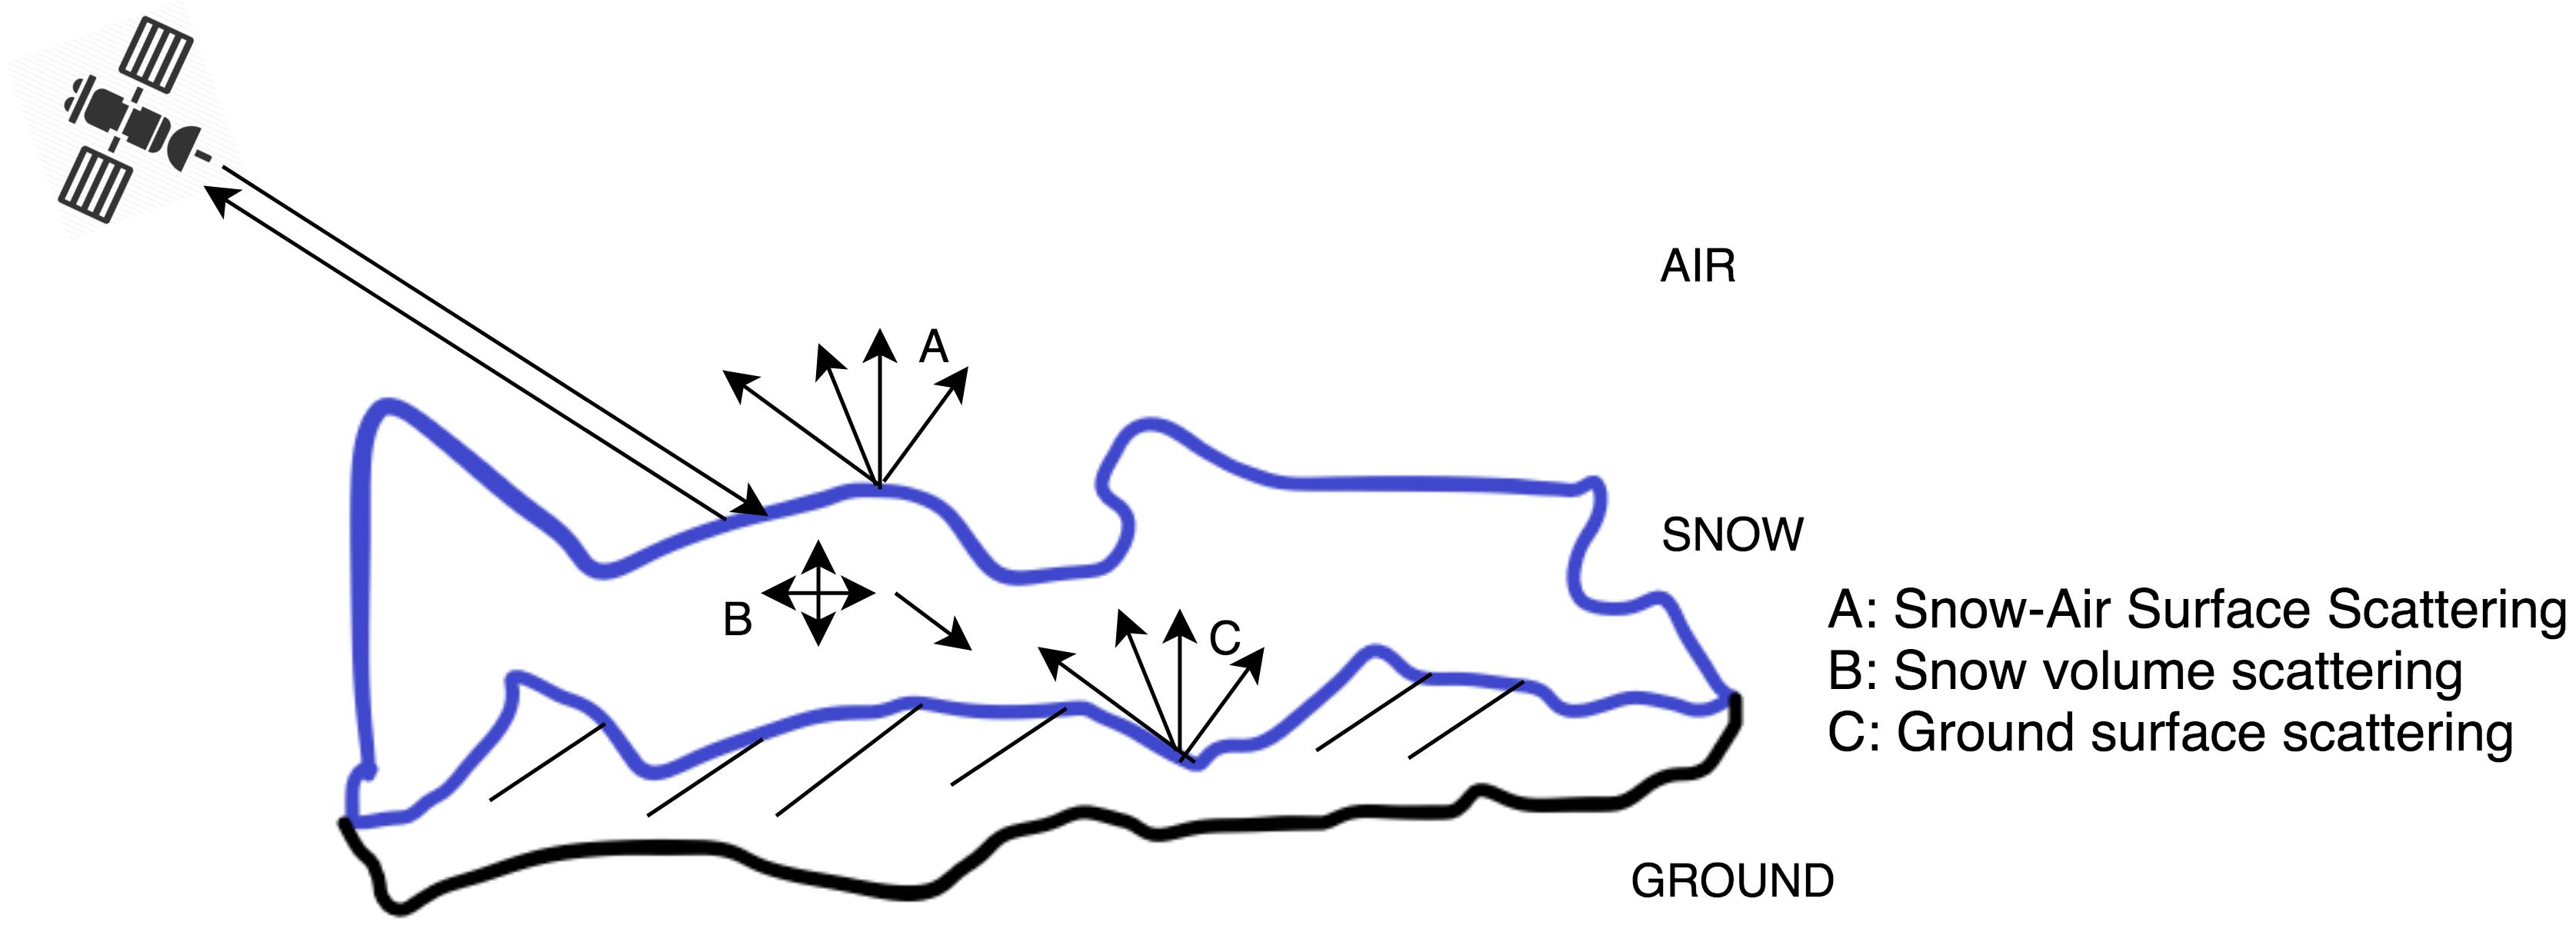
\includegraphics[width=\textwidth]{Figures/Conceptual.png}
    \caption{Conceptual diagram displaying the radar backscattering mechanism in hilly terrains. Adapted from \cite{Thakur2012}.}
    \label{fig:concept}
\end{figure}

PolSAR based algorithms which work on the polarimetric backscatter signal have been widely adopted for various snow related applications such as the classification of dry and wet snow, measuring snow wetness and snow density \citep{Singh2017, Snehmani2010, Thakur2012, Thakur2017, Usami2016}.  \cite{Leinss2014} introduced the use of spaceborne PolSAR for snow height determination, wherein the relationship between the copolar phase difference (CPD) and fresh snow depth is quantitatively analysed by deriving a theoretical model. Moreover, InSAR techniques find significant usage in the cryosphere domain and have been used to measure dry snow depth and SWE in several studies \citep{Conde2018, Guneriussen2001, Leinss2015, Li2017, Liu2017}. In this context, the Pol-InSAR technique works on the coherent combination of both PolSAR and InSAR observations, thereby enabling the interferogram generation in arbitrary transmit and receive channels \citep{Papathanassiou2001, Cloude2005, Cloude2010}. It has been widely used for estimating tree height in forested regions and can be effectively applied to natural or artificial volume scatterers including snow and ice \citep{Leinss2014, Hajnsek2009, Kugler2015, Kumar2017, Papathanassiou2001}.

The prime focus of this research is to estimate the standing snow depth (SSD) using the Pol-InSAR technique. Additionally, the corresponding standing SWE (SSWE) is calculated based on a fixed snow density. In this work, the main innovation lies in improving the Pol-InSAR based hybrid DEM differencing and coherence amplitude inversion model \citep{Cloude2005, Cloude2010, Majumdar2019a}. This model is successfully tested for six fully polarimetric (quad-pol) TerraSAR-X/TanDEM-X \citep{Balss2012} data acquired between December 2015 and January 2016 over Dhundi, situated in the Beas river watershed of the northwestern Himalayas near Manali. The results are obtained after performing thorough sensitivity analysis of the free model parameters. Furthermore, the scattering characteristics of the study area are analysed using the dual-pol entropy ($H$) and scattering angle ($\alpha)$ or $H/{\alpha}$ decomposition, and unsupervised Wishart classification techniques \citep{Lee2009, Cloude2010, Singh2014} for identifying the potential uncertainty sources.

This manuscript is organised in five primary sections and starts with an introductory discussion in section \ref{sec:Intro}. Thereafter, the technical workflow is described in section \ref{sec:method} following which the study area including required datasets and software are specified (section \ref{sec:study}). Finally, the results (section \ref{sec:res}) and the relevant conclusions (section \ref{sec:conc}) are put forward.

\section{Methodology}
\label{sec:method}

This section deals with the methodological framework which has been followed to generate the SSD and SSWE results. The pre-processing steps are briefly discussed in section \ref{ssec:pre} and the Pol-InSAR based approach used for the SSD estimation is addressed in section \ref{ssec:ssd}. Moreover, the uncertainty assessment, validation and sensitivity analysis tasks are described in section \ref{ssec:vus}.

\subsection{Data Preprocessing}
\label{ssec:pre}

Since the SAR datasets are already coregistered, separate coregistration step has not been performed. For the SSD inversion model, the geocoded or terrain-corrected data (3 m spatial resolution) consists of the quad-pol channels, HH, HV, VH, and VV. Additionally, the local incidence angle (LIA) is computed from the ALOS PALSAR DEM (Fig \ref{fig:overview}). It should be noted that, for the Pol-InSAR technique, processing both the TanDEM-X (master) and TerraSAR-X (slave) images \citep{Balss2012} are mandatory for generating the interferogram. The dataset descriptions are provided in section \ref{ssec:data}. 

\subsection{Pol-InSAR based Standing Snow Depth Estimation}
\label{ssec:ssd}

Standing or old snow refers to the deposited snow on the ground which has accumulated over time \citep{Reynolds1983, Majumdar2019a}. Typically, old snow due to the presence of impurity and temperature-gradient induced recrystallisation process consists of snow particles larger than the X-band microwave wavelengths and results in volume scattering \citep{Leinss2016, Riche2013}. This volume decorrelation can be quantitatively analysed with the help of the Pol-InSAR technique \citep{Cloude2010} to obtain the volumetric SSD ($\Delta{Z_s}$). 

\subsubsection{Single-baseline Pol-InSAR Specifics}

The single baseline Pol-InSAR algorithm works on the basis of the complex coherence, $\widetilde{\gamma}\left(\vv{w_1}, \vv{w_2}\right)$, defined in Eq. \eqref{seq:coh} where $I_i\left(\vv{w_1}, \vv{w_2}\right)$ denotes the $i$\textsuperscript{th} pixel coordinate value of the wrapped Pol-InSAR interferogram, $I\left(\vv{w_1}, \vv{w_2}\right)$ obtained in Eq. \eqref{seq:ifg}. This interferogram is calculated from Eq. \eqref{seq:s1} and Eq. \eqref{seq:s2} where the coregistered master ($s_1$) and slave ($s_2$) images are acquired at a given polarisation vector, ($\vv{w}$) respectively. Here, the weight vectors, $\vv{w_1}$ and $\vv{w_2}$ are selected by the user based on the scattering mechanisms at ends 1 and 2 of the interferometric baseline. If $\vv{w_1} = \vv{w_2}$, $\widetilde{\gamma}\left(\vv{w_1}, \vv{w_2}\right)$ can be alternatively specified as $\widetilde{\gamma}\left(\vv{w_1}\right)$ \citep{Cloude2005, Cloude2010}. Moreover, $L$ is the total number of pixels averaged in the range and azimuth directions which can be replaced by the ensemble averaging operation following the statistical ergodicity assumption \citep{Hanssen2001, Hoen2000, Kugler2015, Kumar2017, Papathanassiou2001}. Additionally, $\phi_{flat}^w \in [0, 2\pi)$ is the wrapped flat-earth phase obtained from the estimated absolute flat-earth phase, $\phi_{flat}$ and has to be removed from $I\left(\vv{w_1}, \vv{w_2}\right)$ as shown in Eq. \eqref{seq:ifg}. Also, the calculation of the generalised weight vector, $\vv{w}$ is given by Eq. \eqref{seq:weight}.

\begin{subequations}
    \centering
    \begin{align}
        \label{seq:coh} 
        & \widetilde{\gamma}\left(\vv{w_1}, \vv{w_2}\right) = \frac{\sum_{i=1}^LI_i\left(\vv{w_1}, \vv{w_2}\right)}{\sqrt{\sum_{i=1}^L\left\lvert s_{1i}\left(\vv{w_1}\right)\right\rvert^2\sum_{i=1}^L\left\lvert s_{2i}\left(\vv{w_2}\right)\right\rvert^2}}, \left\lvert\widetilde{\gamma}\left(\vv{w_1}, \vv{w_2}\right)\right\rvert  \in [0, 1] \\
        \label{seq:ifg} 
        & I\left(\vv{w_1}, \vv{w_2}\right) = s_1\left(\vv{w_2}\right)s_2^*\left(\vv{w_2}\right)e^{-j\phi_{flat}^w} \\
        \label{seq:s1} 
        & s_1 = w_1^1\frac{s_{hh}^1 + s_{vv}^1}{\sqrt{2}} + w_1^2\frac{s_{hh}^1 - s_{vv}^1}{\sqrt{2}} + w_1^3\sqrt{2}s_{hv}^1 \\
        \label{seq:s2} 
        & s_2 = w_2^1\frac{s_{hh}^2 + s_{vv}^2}{\sqrt{2}} + w_2^2\frac{s_{hh}^2 - s_{vv}^2}{\sqrt{2}} + w_2^3\sqrt{2}s_{hv}^2 \\
        \label{seq:weight}
        & \vv{w} = \begin{bmatrix}
                    w^1 & w^2 & w^3
                    \end{bmatrix}^T = \begin{bmatrix}
                    \cos\alpha & \sin\alpha \cos{\beta{e}^{j\delta}} & \sin\alpha\sin{\beta{e}^{j\mu}}
                    \end{bmatrix}^T
    \end{align}
\end{subequations}
where, $s_{pp}^1$ and $s_{pp}^2$ correspond to the master (1) and slave (2) images respectively, $pp \in \{hh, hv, vv\}$,
and $*$ denotes the complex conjugate operator.

In this case, the parameters, scattering angle ($\alpha$), target orientation angle ($\beta$), phase terms ($\delta$ and $\mu$), are chosen according to the selected polarisation given by Table \ref{table:1}. LL, LR and RR correspond to the left circular, left-right circular and right circular polarisations \citep{Cloude2010}. However, it is possible to optimise these parameters specific to the data, the details of which are provided by \cite{Cloude2010}.

\begin{table}[ht]
\centering
\caption{Pol-InSAR scattering mechanisms \citep{Cloude2005}.}
\label{table:1}
\begin{tabular}{c c c c c}
\hline
\textbf{Polarisation Selection} & \boldmath$\alpha(^\circ)$   & \boldmath$\beta(^\circ)$     & \boldmath$\delta(^\circ)$ & \boldmath$\mu(^\circ)$       \\ \hline
HH                     & 45 & 0   & 0          & 0   \\ 
HV                     & 90 & 90  & 0          & 0   \\ 
VV                     & 45 & 180 & 0          & 0   \\ 
HH+VV                  & 0  & 0   & 0          & 0   \\ 
HH-VV                  & 90 & 0   & 0          & 0   \\ 
LL                     & 90 & 45  & 0          & 90  \\ 
LR                     & 0  & 0   & 0           & 0   \\ 
RR                     & 90 & 45  & 0          & -90 \\ \hline
\end{tabular}
\end{table}

\subsubsection{Height Inversion Algorithm Details}
In this study, the modified (also improved) hybrid DEM differencing and coherence amplitude based Pol-InSAR volumetric height inversion model as given by Eq. \eqref{seq:hybrid_dem} is used for the SSD estimation \citep{Majumdar2019a}. The modelling details are described only for the January 8, 2016 data. The other quad-pol datasets were analysed after successive iterations keeping most of the hyperparameter values same. 

Firstly, the volume scattering dominant channels, HV and VH, are averaged to fully utilise the quad-pol data \citep{Cloude2005}. Next, the Pol-InSAR interferogram, $I\left(\vv{w_v}\right)$ has been computed using Eq. \eqref{seq:ifg} wherein, the weight vector, $\vv{w_v}$ is obtained from Table \ref{table:1} for the HV polarisation. Thereafter, the complex volume coherence, $\widetilde{\gamma}\left(\vv{w_v}\right)$, is calculated from Eq. \eqref{seq:coh} with $L$ = 3. Similarly, the complex surface or ground coherence, $\widetilde{\gamma}\left(\vv{w_s}\right)$, is computed by choosing $\vv{w_s}$ as the HH-VV weight vector (Table \ref{table:1}). Moreover, the actual vertical wavenumber, $k_z$, when varied with the LIA, is in the order of 0.1 rad/m with the ambiguity height, $h_{2\pi} = 2\pi/k_z \approx$ 63.18 m, $\lambda_0 \approx$ 3.11 cm and $m$ = 1 (single-pass acquisition). Since the maximum height of the distributed volume scatterer (in this case, standing snow), $\Delta{Z_{s,max}}$, should be similar to $h_{2\pi}$ \citep{Kugler2015, Hajnsek2009, Kumar2017}, $k_z$ has to be rescaled to an optimum range for effectively estimating the SSD. Hence, the modified vertical wavenumber, $k_z^\prime$ , is given by Eq. \eqref{seq:vn} where $\eta^\prime$ is a free scaling parameter which has to be set according to the known $\Delta{Z_{s,max}}$ in the study area. Here, $h_{2\pi}^\prime$ is the scaled height of ambiguity which like that of $h_{2\pi}$ determines the height changes in modulo $2\pi$ \citep{Hanssen2001}. Also, $\mathbb{R}_{>0}^+$ denotes the set of all positive real numbers in the interval $(0, \infty)$. In this work, due to the limited ground-truth data availability and the subsequent ensemble averaging operation (window size of 21$\times$21) on $k_z^\prime$ , $\Delta{Z_{s,max}} = $ 12 m has been assumed for which $\eta^\prime = $ 5 is used. It should be noted that the selection of these parameter values have been carried out after appropriate sensitivity analysis which is discussed in section \ref{ssec:sar}.

Apart from this, the function $\arg$ is defined in the interval $[0, 2\pi)$ and the parameter $m$ is set to 1 for bistatic acquisition and 2 in the monostatic case. Also in Eq. \eqref{seq:vn}, $\Delta\theta$ is the change in the incidence angle occuring due to the spatial baseline, $\theta_l$ is the LIA, and $\lambda_0$ is the radar wavelength \citep{Cloude2010, Kugler2015}.

\begin{subequations}
    \centering
    \begin{equation}
        \label{seq:hybrid_dem}
        \Delta{Z_s} = \frac{\arg\left(\widetilde{\gamma}\left(\vv{w_v}\right)e^{-j\phi_{topo}^w}\right)}{k_z^\prime} + \eta\frac{\sinc_\pi^{-1}\left(\gamma\left(\vv{w_v}\right)\right)}{k_z^\prime}, \eta\in[0, 1]
    \end{equation}
    \begin{flushleft}\text{where,}\end{flushleft}
    \begin{equation}
        \label{seq:vn}
        k_z^\prime = \left\langle\eta^\prime\frac{m\Delta\theta}{\lambda_0\sin\theta_l}\right\rangle, \eta^\prime\in\mathbb{R}_{>0}^+\mid\Delta{Z_{s, max}} \approx h_{2\pi}^\prime = 2\pi/k_z^\prime
    \end{equation}
\end{subequations}

Subsequently, the volume and surface coherences are then used to estimate the wrapped ground phase, $\phi_{topo}^w \in [0, 2\pi)$, from Eq. \eqref{eq:topo}. Additionally, a median ensemble filter of 21$\times$21 is applied on the obtained $\phi_{topo}^w$ following the processing steps provided by \cite{Cloude2005}.

\begin{equation}
    \label{eq:topo}
    \phi_{topo}^w = \arg\left(\widetilde{\gamma}\left(\vv{w_v}\right) - \widetilde{\gamma}\left(\vv{w_s}\right)\left(1 - L_{\vv{w_s}}\right)\right)
\end{equation}
where,
\begin{align*}
    & L_{\vv{w_s}} = \frac{-B - \sqrt{B^2 - 4AC}}{2A}, L_{\vv{w_s}} \in [0, 1] \\
    & A = \left\lvert\widetilde{\gamma}\left(\vv{w_v}\right)\right\rvert^2 - 1 \\
    & B = 2\Re\left(\widetilde{\gamma}\left(\vv{w_v}\right) - \widetilde{\gamma}\left(\vv{w_s}\right)\widetilde{\gamma}^*\left(\vv{w_v}\right)\right) \\
    & C = \left\lvert\widetilde{\gamma}\left(\vv{w_v}\right) - \widetilde{\gamma}\left(\vv{w_s}\right)\right\rvert^2
\end{align*}

Eventually, the SSD ($\Delta{Z_s}$) and SSWE ($=\rho_s\Delta{Z_s}$) are estimated wherein the standing snow density ($\rho_s = $ 0.315 g/cm\textsuperscript{3}) measured by the Dhundi SPA at 00:52 hrs UTC on January 8, 2016, has been used (Table \ref{table:ssd_data}). Here, $\eta = $ 0.65, the volume coherence threshold, $\tau_v = $ 0.6 (pixels having $\tau_v < $ 0.6 are neglected $\forall\tau_v \in$ [0, 1]), and the SSD values are averaged based on a 57$\times$57 ensemble filter window. The entire Pol-InSAR workflow is summarised in Figure \ref{fig:ssd_method} which shows the main processing blocks.

\begin{figure}[htb]
    \centering
    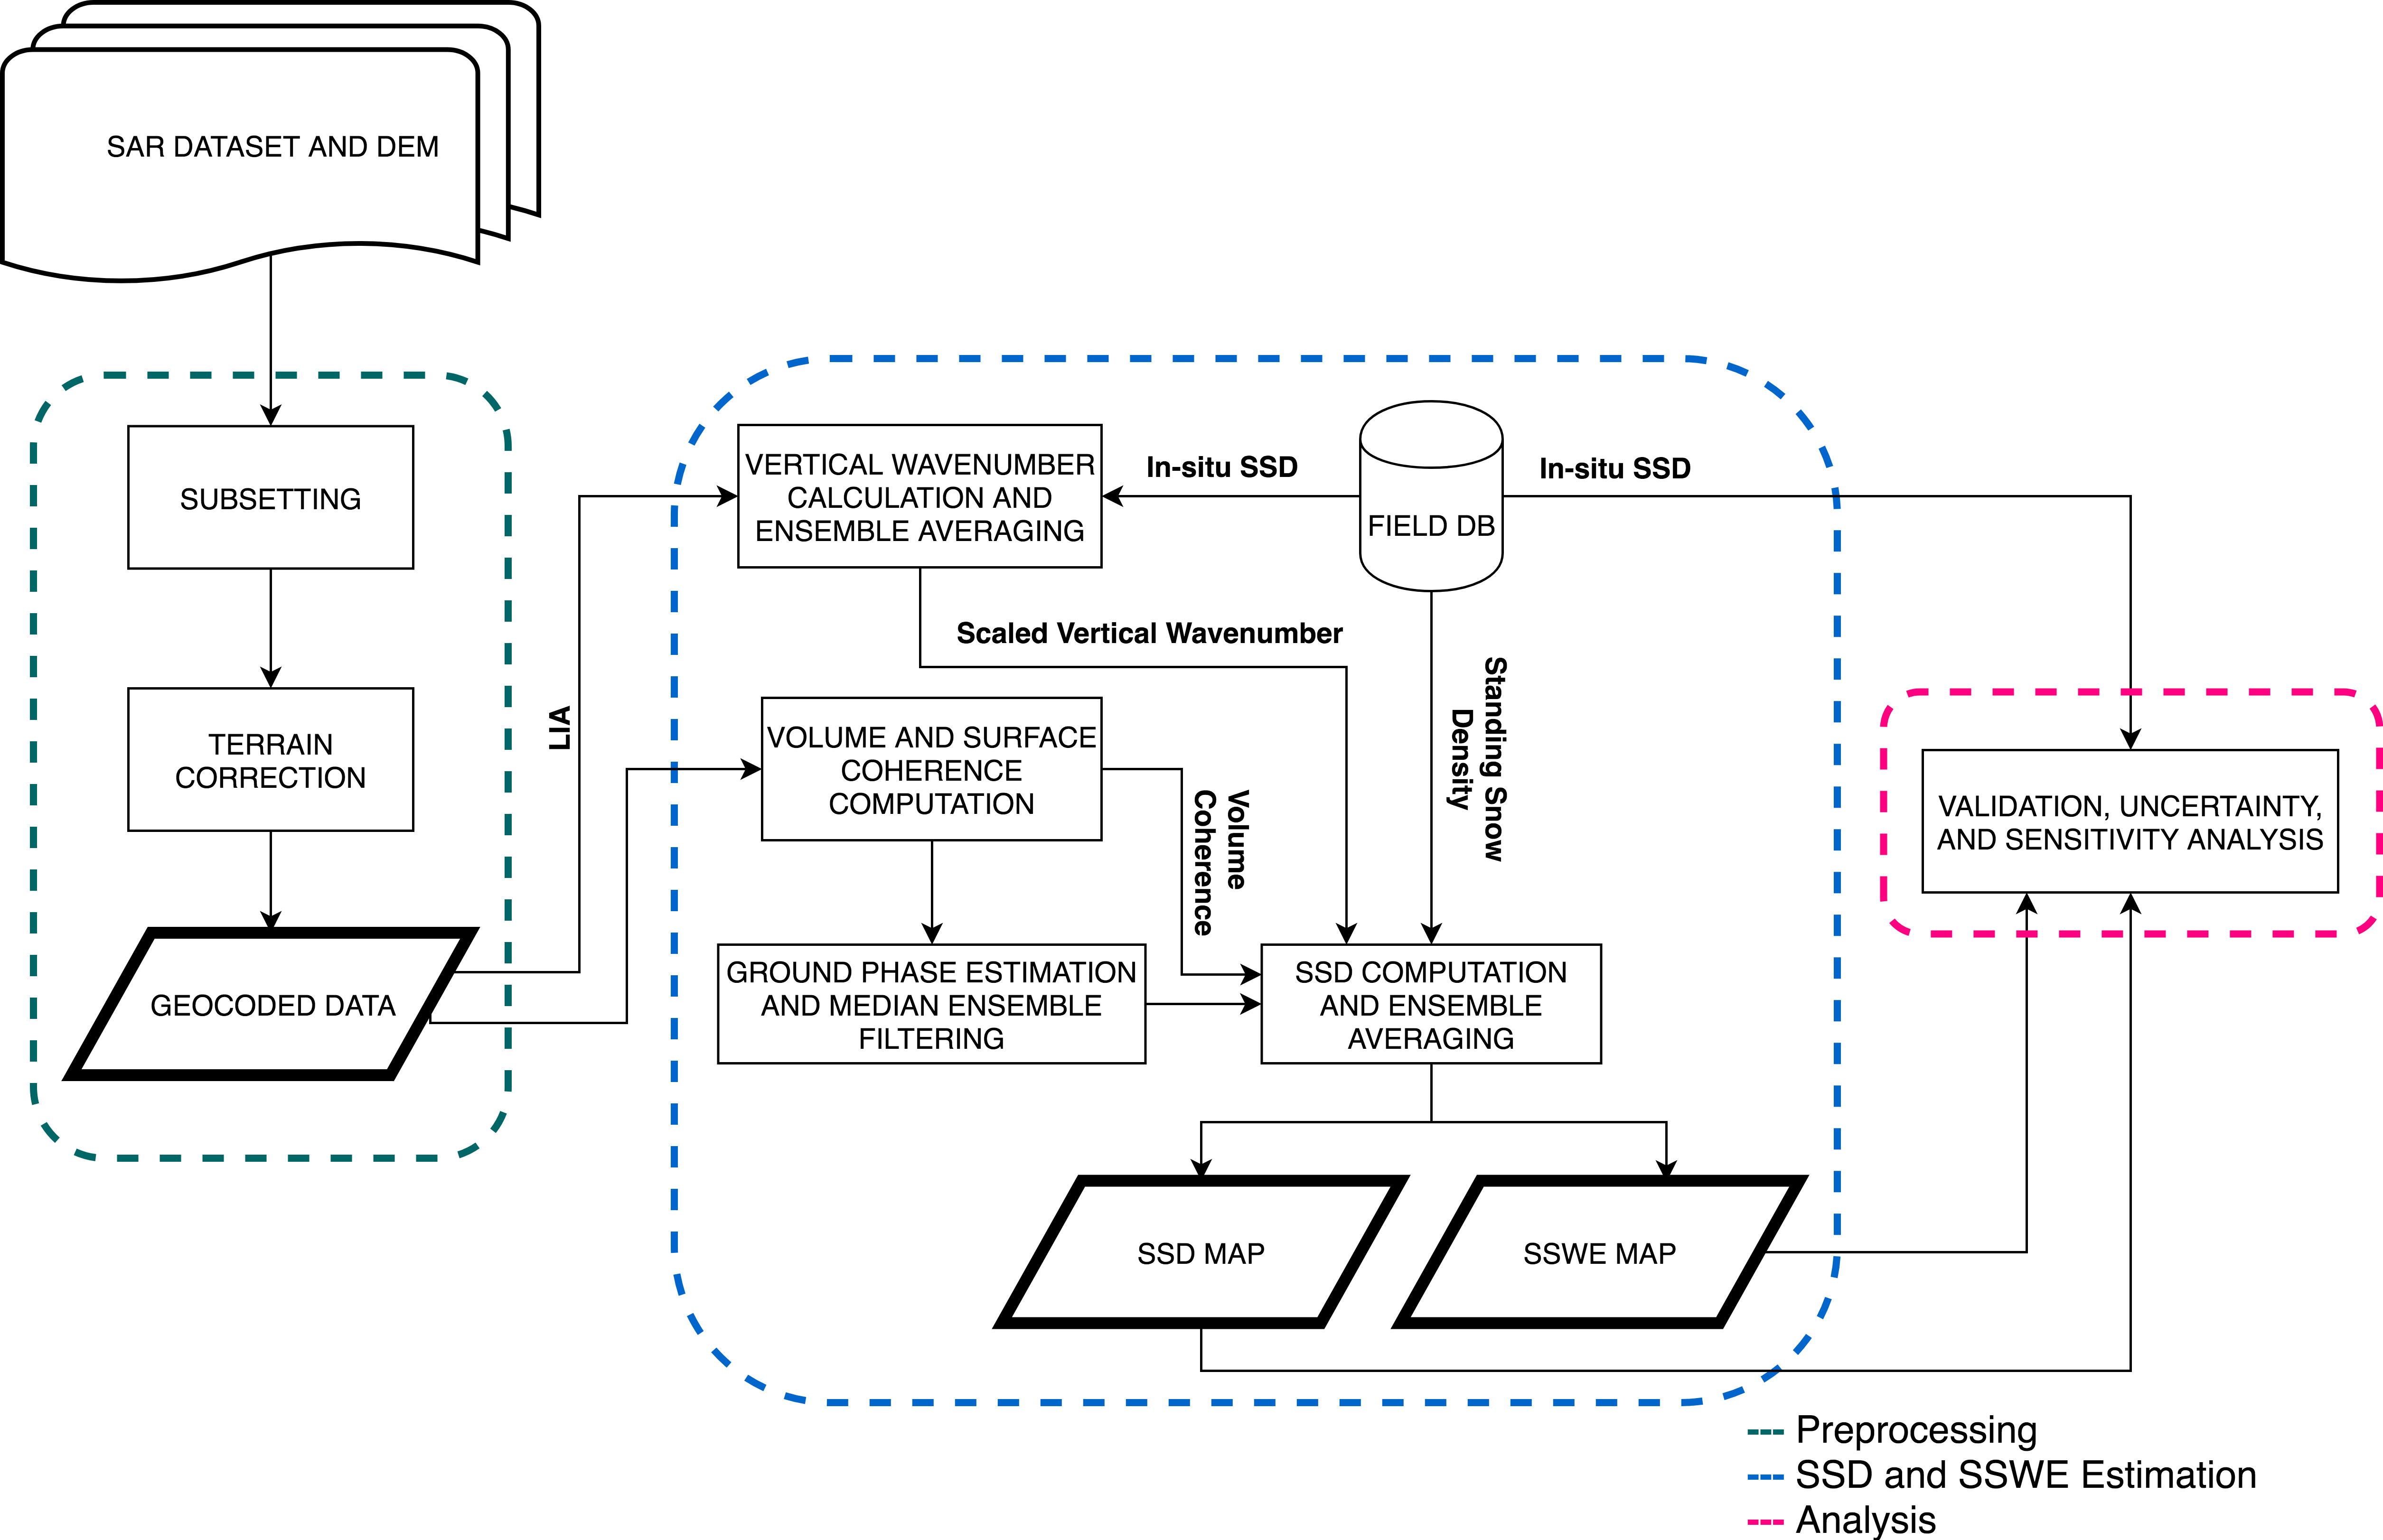
\includegraphics[width=\textwidth]{Figures/Methods/SSD_Method.png}
    \caption{SSD and SSWE estimation workflow using Pol-InSAR.}
    \label{fig:ssd_method}
\end{figure}

However, in order to compute the inverse $\sinc_\pi$ (normalised $\sinc$) function in Eq. \eqref{seq:hybrid_dem}, the \cite{Cloude2010} approximation ($\sinc_C^{-1}$) in Eq. \eqref{seq:un_cloude} is replaced by Eq. \eqref{seq:secant} where the secant method \citep{Cheney2012} has been applied to find $\alpha_r \in \mathbb{R}$ (rad), the desired root or inverse. Moreover, to make the \cite{Cloude2010} approximation compliant with the scientific computing libraries such as SciPy \citep{Jones2001} which use the $\sinc_\pi$ function, the normalised variant of Eq. \eqref{seq:un_cloude} given by Eq. \eqref{seq:ncloude} is incorporated where $\sinc_{\pi_C}^{-1}$ denotes the inverse of the $\sinc_\pi$ function computed using the \cite{Cloude2010} approach. Similarly, $\sinc_{\pi_S}^{-1}$ represents the inverse of the $\sinc_\pi$ function obtained by applying the secant method \citep{Cheney2012, Jones2001}. This root finding technique has been deployed as it is more accurate than the given approximation in Eq. \eqref{seq:ncloude}, the analysis of which is described in section \ref{sssec:sinc}. Still, in the Python implementation, this approximation is used as an initial guess to the secant method for faster convergence. It is also used as a fallback option if the secant method is unable to converge within 50 iterations or the default convergence threshold of 1.4E-8 \citep{Jones2001}.

\begin{subequations}
    \centering
    \begin{align}
        \label{seq:un_cloude}
        & \sinc_C^{-1}\left(\gamma\left(\vv{w_v}\right)\right) = \pi - 2\sin^{-1}\left(\gamma\left(\vv{w_v}\right)^{0.8}\right) \\
        \label{seq:secant}
        & \sinc_\pi\alpha_r  - \gamma\left(\vv{w_v}\right) = 0 \\
        \label{seq:ncloude}
        & \sinc_{\pi_C}^{-1}\left(\gamma\left(\vv{w_v}\right)\right) = \frac{\sinc_C^{-1}\left(\gamma\left(\vv{w_v}\right)\right)}{\pi}
    \end{align}
\end{subequations}

\subsection{Validation, Uncertainty Assessment, and Sensitivity Analysis}
\label{ssec:vus}
\subsubsection{Validation Process}
\label{sssec:val}

One of the significant challenges in this work is the limited ground-truth data availability. Since, in-situ data from only two ground stations are available, the conventional way of accuracy assessment through regression plots \citep{Kugler2015, Leinss2014, Kumar2017} is infeasible in this context. Moreover, the Kothi AWS (Fig \ref{fig:overview}) area falls in the layover region for the descending pass acquisitions and hence, only the Dhundi region which is free from layover, shadow and foreshortening effects, is used for validation. In this case, a neighbourhood window of size 3$\times$3 ($\approx$ 81 m\textsuperscript{2} ground area) surrounding the Dhundi SPA is selected for validating the SSD and SSWE estimates by considering only the statistical mean and standard deviation.

\subsubsection{Uncertainty Assessment}
\label{sssec:ua}

Due to the complex terrain characteristics there exist significant uncertainty sources which could potentially lead to the overall degradation of the output accuracy. Having the quad-pol data in winter time (January 8, 2016) and dual-pol data in summer time, we are able to use dual-pol entropy ($H \in$ [0, 1]) and the scattering alpha angle ($\alpha \in$ [0$^\circ$, 90$^\circ$]) or $H/{\alpha}$ decomposition to comparatively understand the backscattering mechanisms in these two time intervals \citep{Cloude2010, Lee2009, Singh2014}. The 5$\times$5 window size for the $H/{\alpha}$ decomposition is used. This is carried out through the $H/{\alpha}$ plane plot which demarcates eight feasible zones (Z9 being the unclassified pixels) based on the different scattering classes as shown in Figure \ref{fig:ha}. Note that, this diagram which follows the SNAP style \citep{ESA2019}, uses slightly different labels as compared to the \cite{Lee2009} $H/{\alpha}$ plane convention where the labels Z1, Z2, Z3 are denoted as Z7, Z8, Z9 and vice-versa respectively. However, the scattering mechanisms are exactly the same in both these conventions. Also, the blue curve acts as a boundary to the plane which essentially denotes the reliability of the classification in high entropy conditions \citep{Brunner2009}.

\begin{figure}[htb]
    \centering
    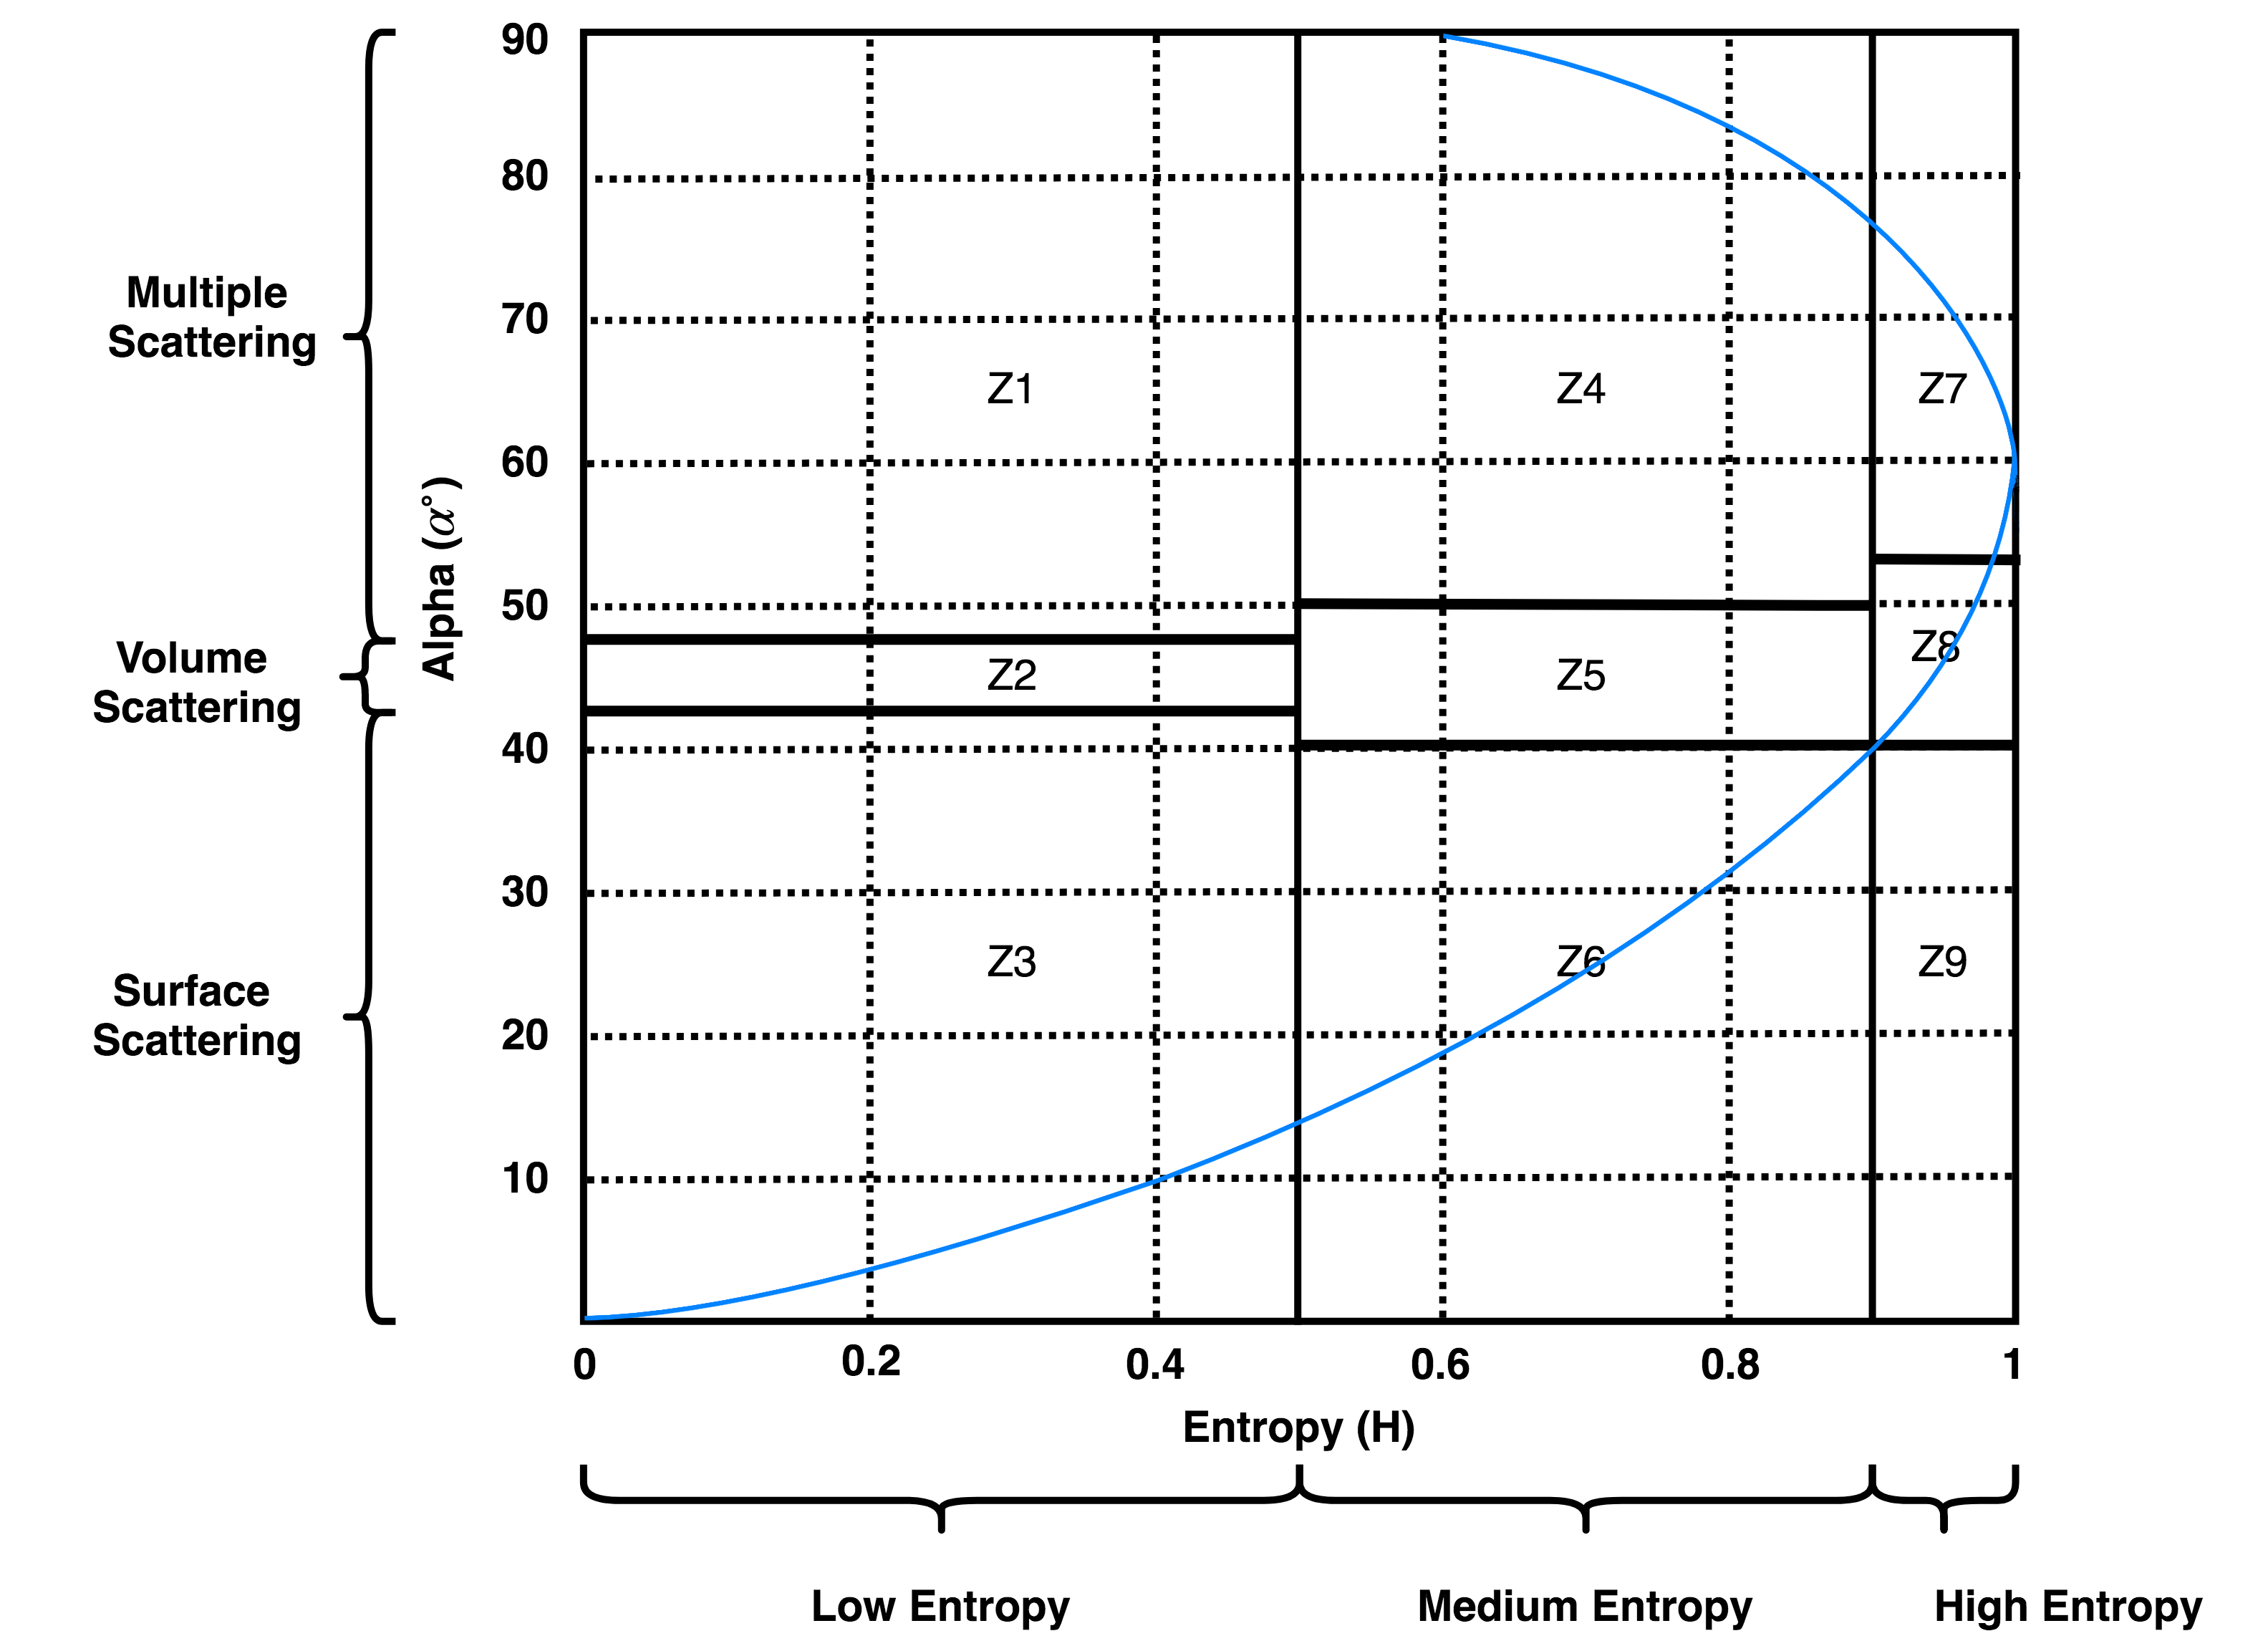
\includegraphics[width=\textwidth]{Figures/Methods/HA.png}
    \caption{$H/{\alpha}$ plane showing different scattering zones. Z1: Dihedral, Z2: Dipole, Z3: Bragg Surface, Z4: Double
bounce, Z5: Anisotropic, Z6: Random surface, Z7: Complex structures, Z8: Random anisotropic, Z9: Non-feasible.}
    \label{fig:ha}
\end{figure}

The dual-pol $H/{\alpha}$ decomposition is further used by the unsupervised Wishart classifier (ten iterations) which classifies the SAR data based on these scattering mechanisms and a quantitative estimate of the number of pixels in each such class can be obtained \citep{Cloude2010, Lee2009}. Therefore, by knowing the scattering properties, the terrain features present in the study area can be understood along with their changes during the snow season. In turn, these ground features which include rough surfaces, shrubs, boulders, and human settlements reduce the Pol-InSAR surface coherence amplitude, $\left(\gamma\left(\vv{w_v}\right) = \left\lvert\widetilde{\gamma}\left(\vv{w_v}\right)\right\rvert\right)$ which may result in overestimated volumetric height (SSD) \citep{Cloude2010, Hajnsek2009, Kugler2015}. Hence, a summer and winter time surface coherence comparison (volume coherence cannot be computed for the summer time datasets because these are dual-pol, Table \ref{table:data}) is also performed to further analyse the effects of these ground features. Thus, the uncertainty assessment by means of the identification of the backscattering mechanisms constitutes a key role in this work.

Apart from this, the forest cover map (obtained from WRD, IIRS) along with the layover and shadow regions computed using SAR simulation are used to mask out the noisy pixels which degrade the quality of the results. This is a standard approach used in the studies focusing on snow property estimation in forested or alpine terrains \citep{Leinss2014, Leinss2016, Singh2017, Thakur2012, Usami2016}.

\subsubsection{Sensitivity Analysis}
\label{sssec:sa}

The variation of the SSD and SSWE values corresponding to the changes in the free parameters in the SSD inversion model (window size, coherence threshold, scaling factors) are observed by iteratively running the algorithm and computing the statistical mean and standard deviation using the neighbourhood window discussed earlier in section \ref{sssec:val}. This helps in deciding the window shape and sizes and also choosing the optimum values for the several free parameters. Moreover, the accuracy of the root finding algorithm discussed in section \ref{ssec:ssd} is also checked for some possible coherence values (section \ref{sssec:sinc}).

In addition, the ground elevation measurements acquired during the field visit to Dhundi and Kothi were compared with the ALOS PALSAR DEM elevations ($z$). The effect of the DEM errors on the LIA, $\theta_l$, is then checked for performing the sensitivity analysis using Eq. \eqref{eq:sa} which incorporates the slope angles in $x$ ($\omega_x$) and $y$ ($\omega_y$) directions (pixel co-ordinate system where $z$ is the corresponding elevation value) derived from the DEM elevation values along with the radar incidence angle ($\theta$) \citep{Lee2000, Lee2009}. Here, the terms $\mathrm{d}z/\mathrm{d}x$ and $\mathrm{d}z/\mathrm{d}y$ refer to the rate of elevation ($z$) change in the $x$ and $y$ directions respectively.

\begin{equation}
    \centering
    \label{eq:sa}
    \theta_l = \cos^{-1}\frac{\cos\omega_x\cos\left(\omega_y - \theta\right)}{\sqrt{\cos^2\omega_y\sin^2\omega_x + \cos^2\omega_x}}
\end{equation}
where, 
\begin{equation*}
    \centering
    \omega_x = \tan^{-1}\frac{\mathrm{d}z}{\mathrm{d}x}, \omega_y = \tan^{-1}\frac{\mathrm{d}z}{\mathrm{d}y}.
\end{equation*}

\section{Study Area, Datasets, and Software}
\label{sec:study}

\subsection{Chosen Study Area}
\subsubsection{Geographical Situation}
\label{sssec:geo}
The Beas river watershed near Manali, India is part of the north-western Himalayas. Naturally, steep slopes and dense forests are prominent in this region. The elevation typically varies from nearly 2500 m to more than 5000 m in some places as observed in the reference ALOS PALSAR DEM (Figure \ref{fig:overview}). 

\begin{figure}[htb]
    \centering
    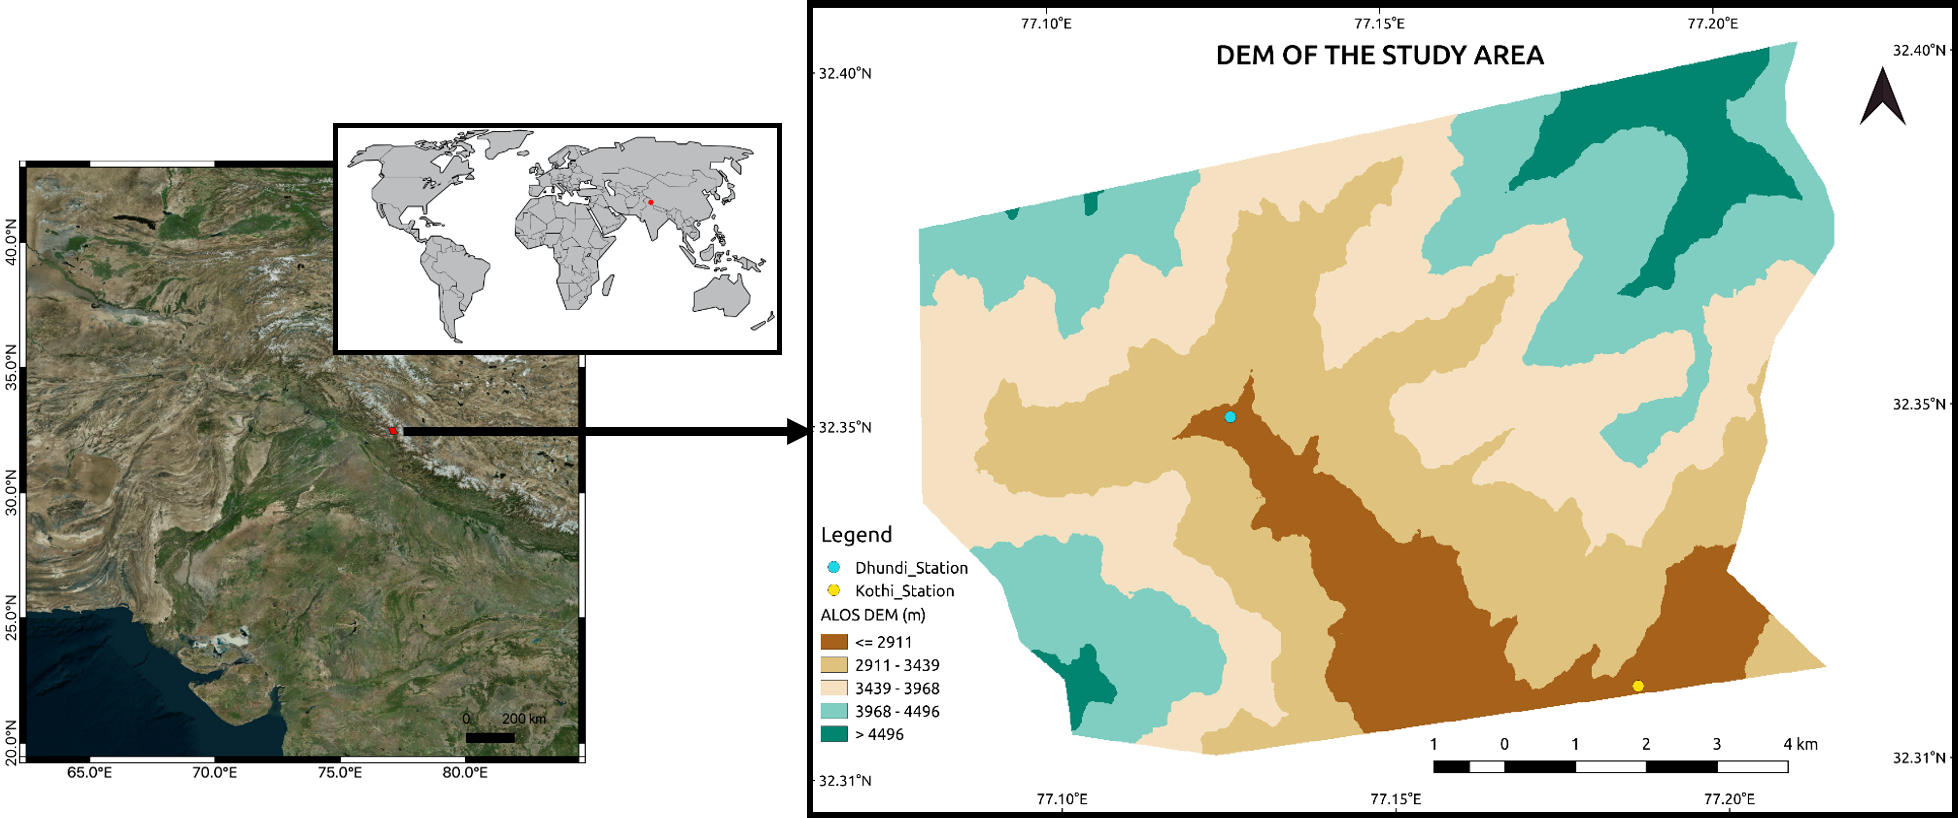
\includegraphics[width=\textwidth]{Figures/Overview.png}
    \caption{Overview map of the study area showing the ALOS PALSAR DEM. The original DEM of 12.5 m spatial resolution (generated in 2011) has been resampled to 3 m using bilinear interpolation \citep{Wu2008} to match the high resolution SAR data. Moreover, the vertical resolution as per the product specification is 5 m.}
    \label{fig:overview}
\end{figure}

In this work, a small region ($\sim$96 km\textsuperscript{2}) of the Beas basin is chosen which starts a few kilometres uphill from Dhundi up to Kothi (shown in Figure \ref{fig:overview}). These areas receive substantial seasonal snowfall which begins in December and lasts till late March. However, the cold, dry season usually commences from late September or early October. The coldest period is in January during which the temperatures reach a daily minimum of -15$^\circ$C on an average. The summers are mild to occasionally warm with June being the hottest month (mean and maximum temperatures of 20$^\circ$C and 30$^\circ$C respectively are common). Apart from this, significant rainfall occurs between late June and September (monsoon season) with August receiving the maximum precipitation \citep{Majumdar2019, Thakur2012}.

\subsubsection{Field Visit}
\label{sssec:field}
Intensive fieldwork had been conducted from October 14-21, 2018 in the Dhundi and Kothi areas where several Differential Global Positioning System (DGPS) measurements were acquired using the Leica Viva GS 10 \citep{LeicaGeosystemsAG2012} with adequate horizontal positional accuracies ($\sim$7 cm) \citep{Majumdar2019}. Due to the complex terrains, most of the DGPS readings had been obtained through the kinematic mode \citep{Luo2014}. However, in some of the convenient places such as the Dhundi base station and near the Kothi Automatic Weather Station (AWS), the static mode was used \citep{LeicaGeosystemsAG2012}. Eventually, elevation information from these DGPS points have been compared with the ALOS PALSAR DEM, the details of which are provided in section \ref{sssec:error}. In order to properly understand and visualise the characteristics of the study area, selected field photographs and their brief description are shown from figures \ref{subfig:gps}-\ref{subfig:stations}.

\begin{figure}[!t]
    \centering
    \begin{subfigure}[t]{0.49\textwidth}
        \raisebox{-\height}{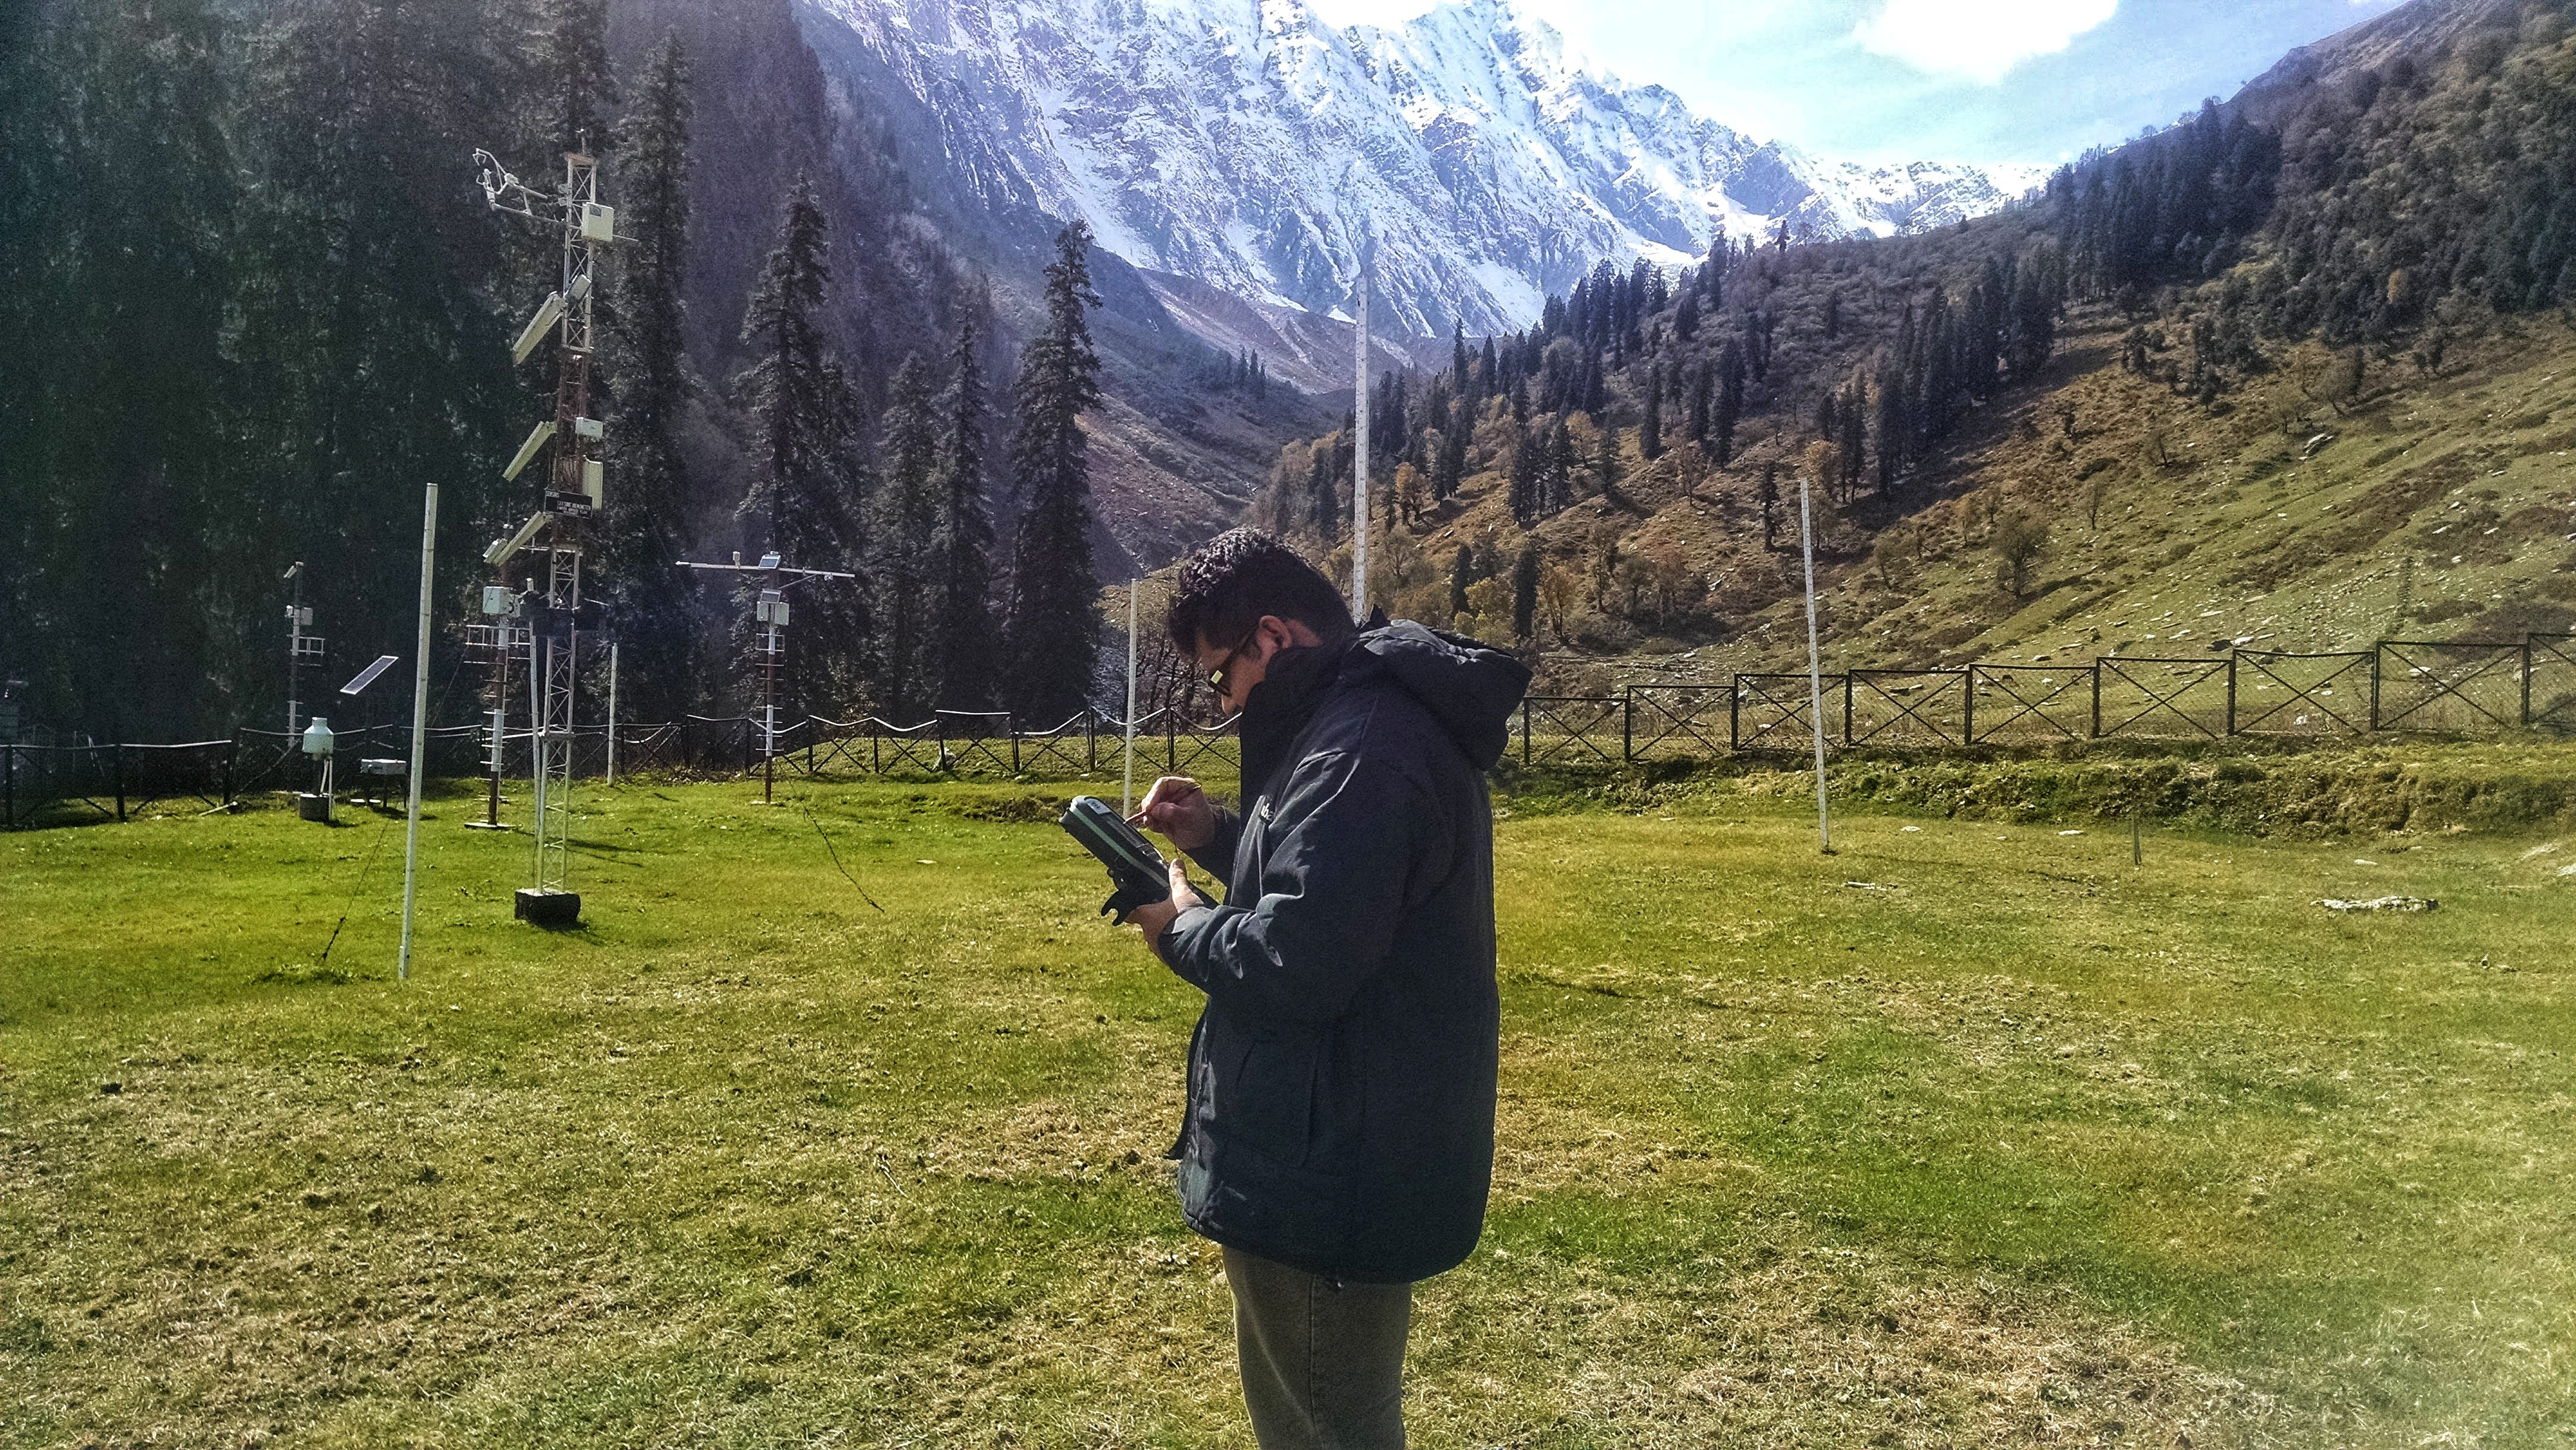
\includegraphics[width=\textwidth]{Figures/Field/me_gps.jpg}}
        \caption{DGPS positional accuracy checking}
        \label{subfig:gps}
    \end{subfigure}
    \hfill
    \begin{subfigure}[t]{0.49\textwidth}
        \raisebox{-\height}{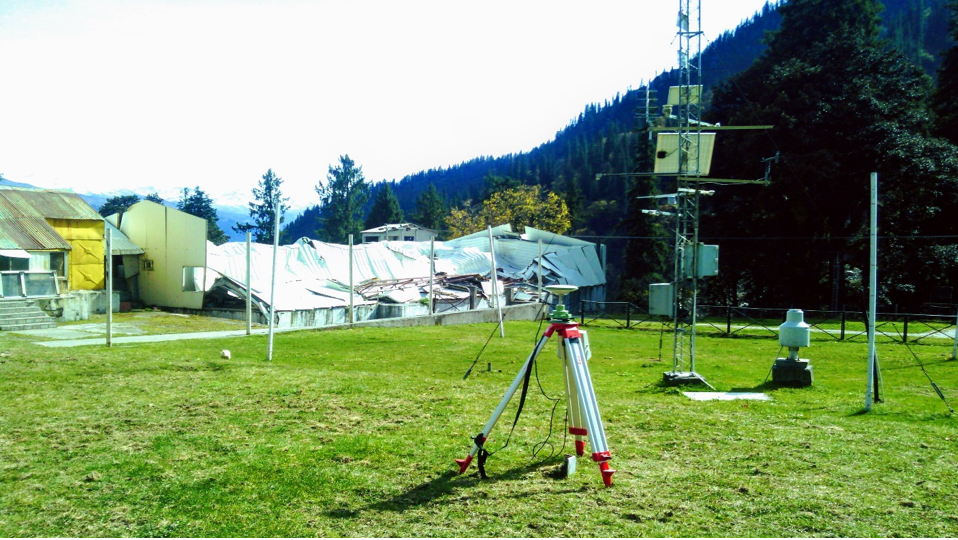
\includegraphics[width=\textwidth]{Figures/Field/base.png}}
        \caption{Leica DGPS base}
        \label{subfig:base}
    \end{subfigure}
    %%%%%%%%%%%%%%%%%%%%%%%%%%%%%%%%%%%%second row
    \begin{subfigure}[t]{0.49\textwidth}
        \raisebox{-\height}{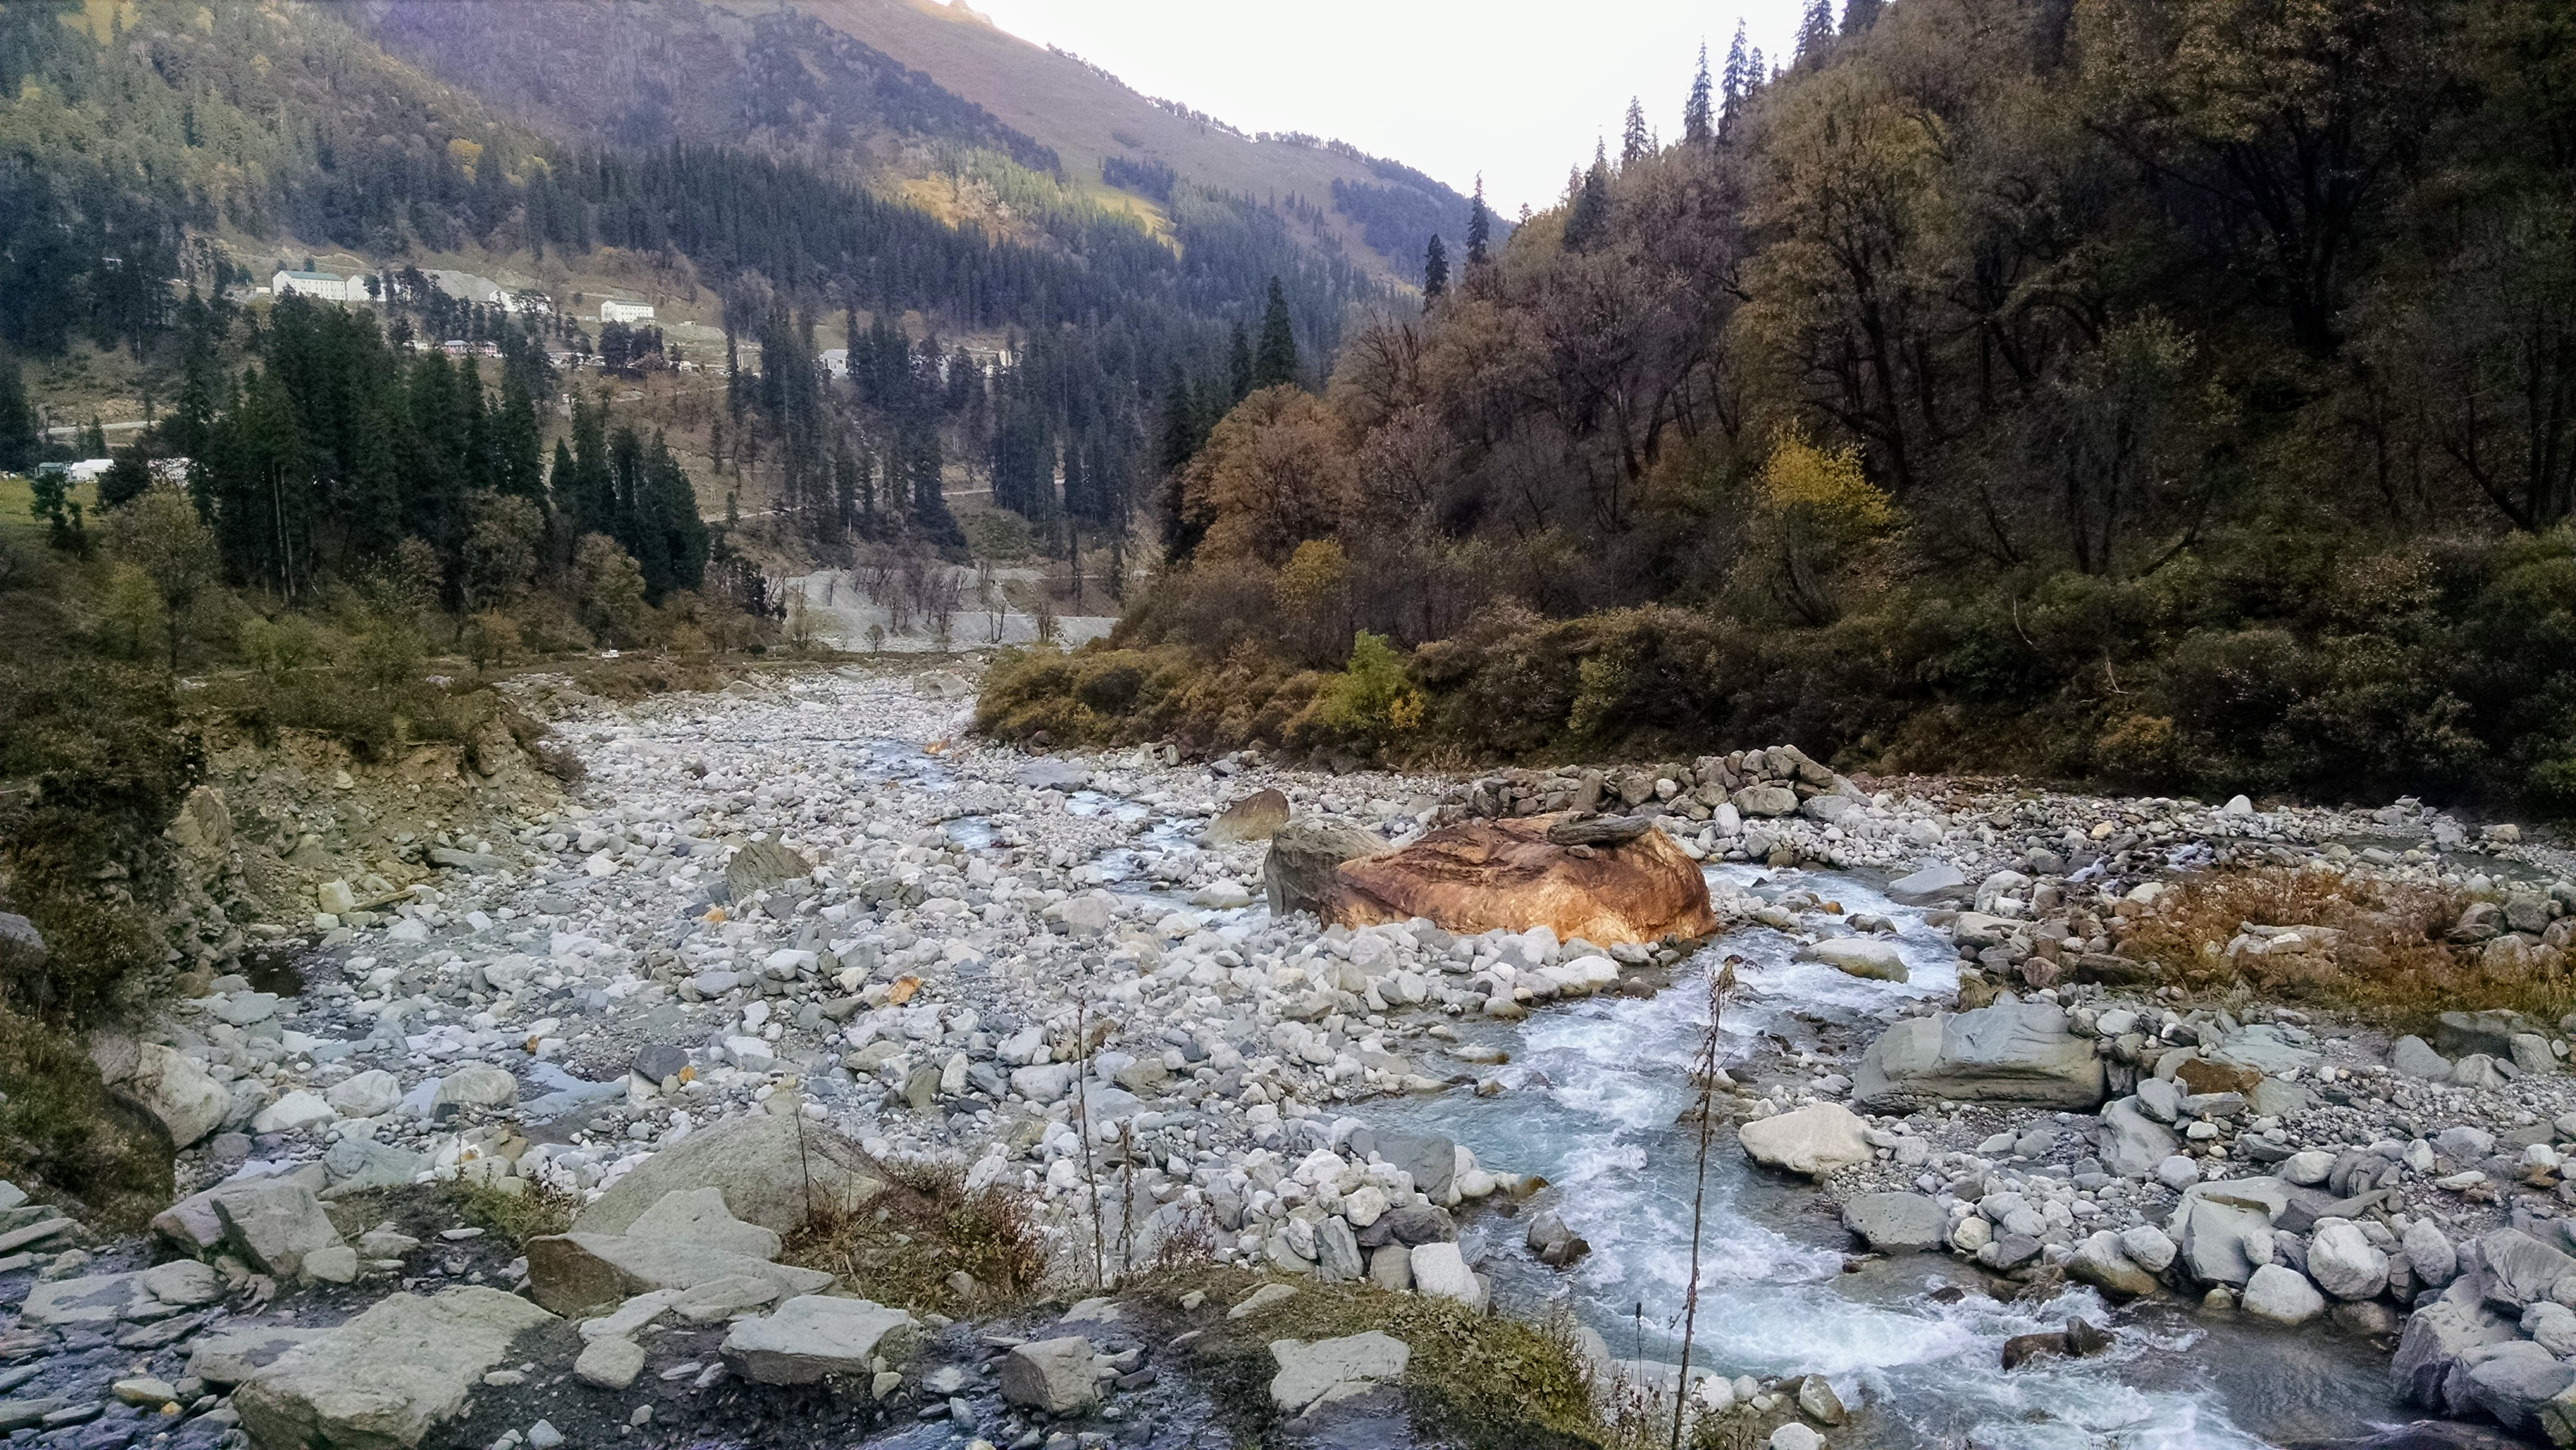
\includegraphics[width=\textwidth]{Figures/Field/beas.jpg}}
        \caption{Beas river}
        \label{subfig:beas}
    \end{subfigure}
    \hfill
    \begin{subfigure}[t]{0.49\textwidth}
        \raisebox{-\height}{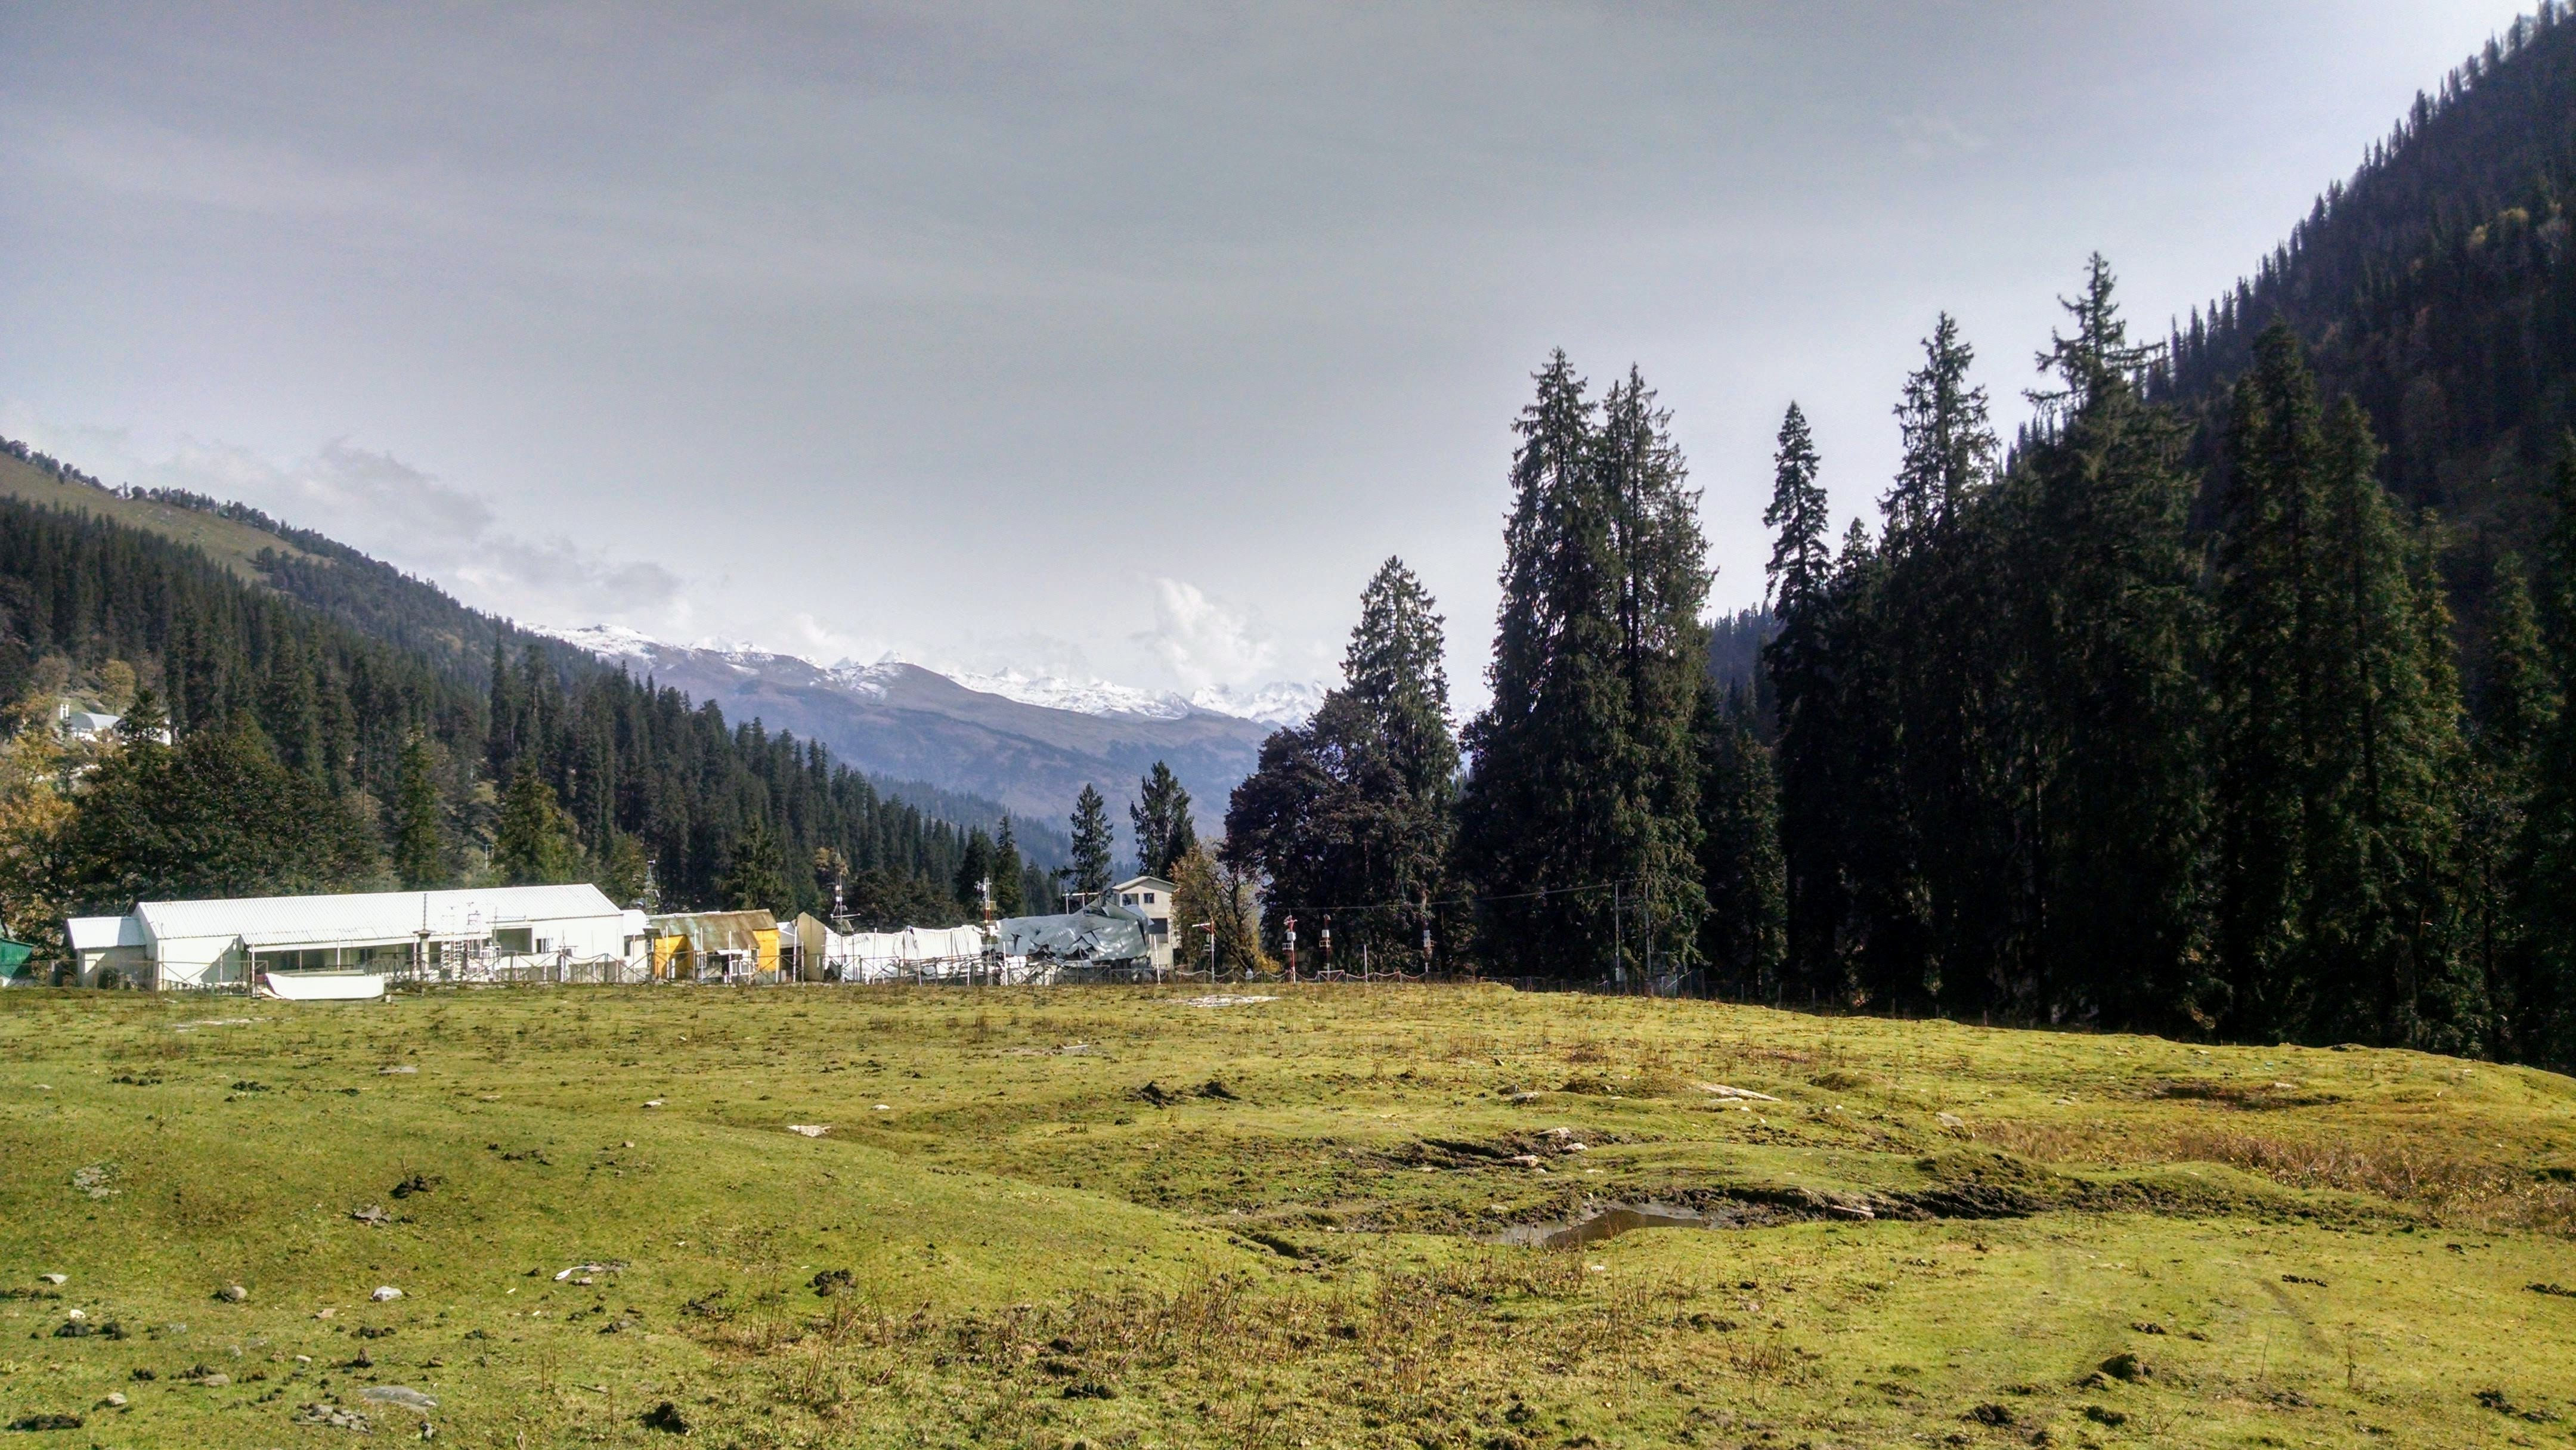
\includegraphics[width=\textwidth]{Figures/Field/landscape.jpg}}
        \caption{Landscape and human settlements}
        \label{subfig:landscape}
    \end{subfigure}
    %%%%%%%%%%%%%%%%%%%%%%%%%%%%%%%%%%%third row
    \begin{subfigure}[t]{0.49\textwidth}
        \raisebox{-\height}{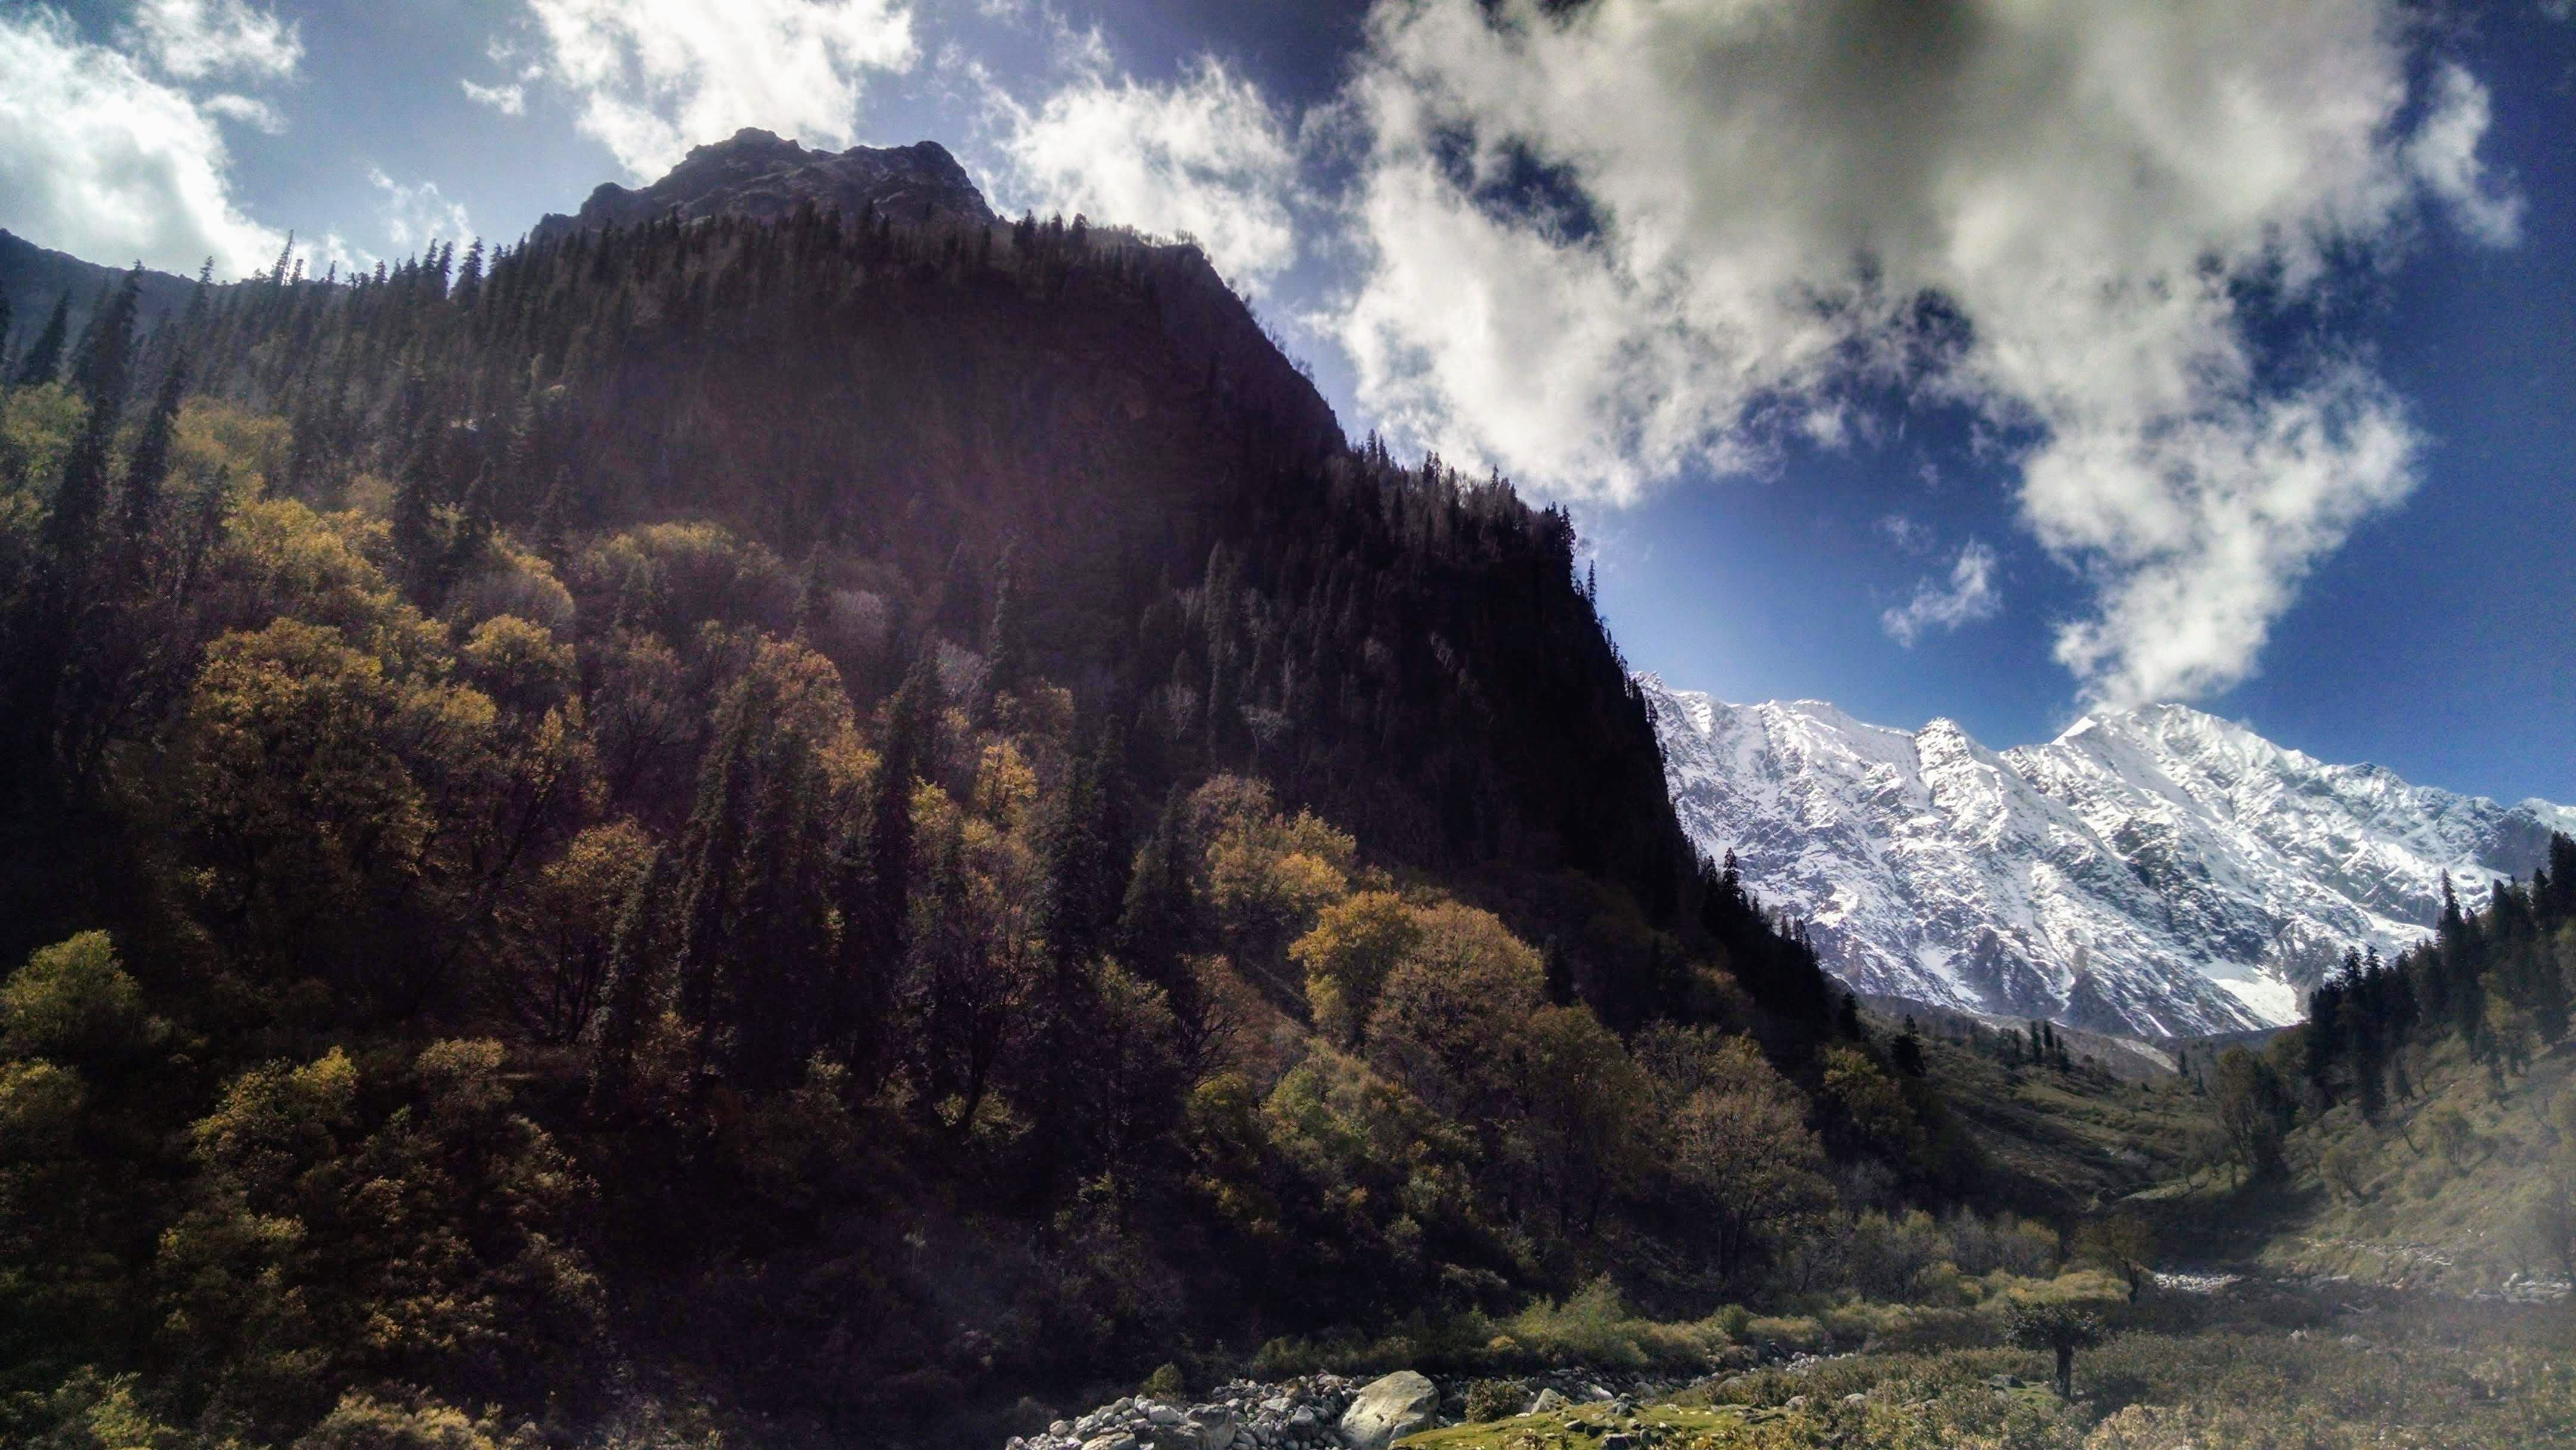
\includegraphics[width=\textwidth]{Figures/Field/mountain.jpeg}}
        \caption{Mountains and forests}
        \label{subfig:mountain}
    \end{subfigure}
    \hfill
    \begin{subfigure}[t]{0.49\textwidth}
        \raisebox{-\height}{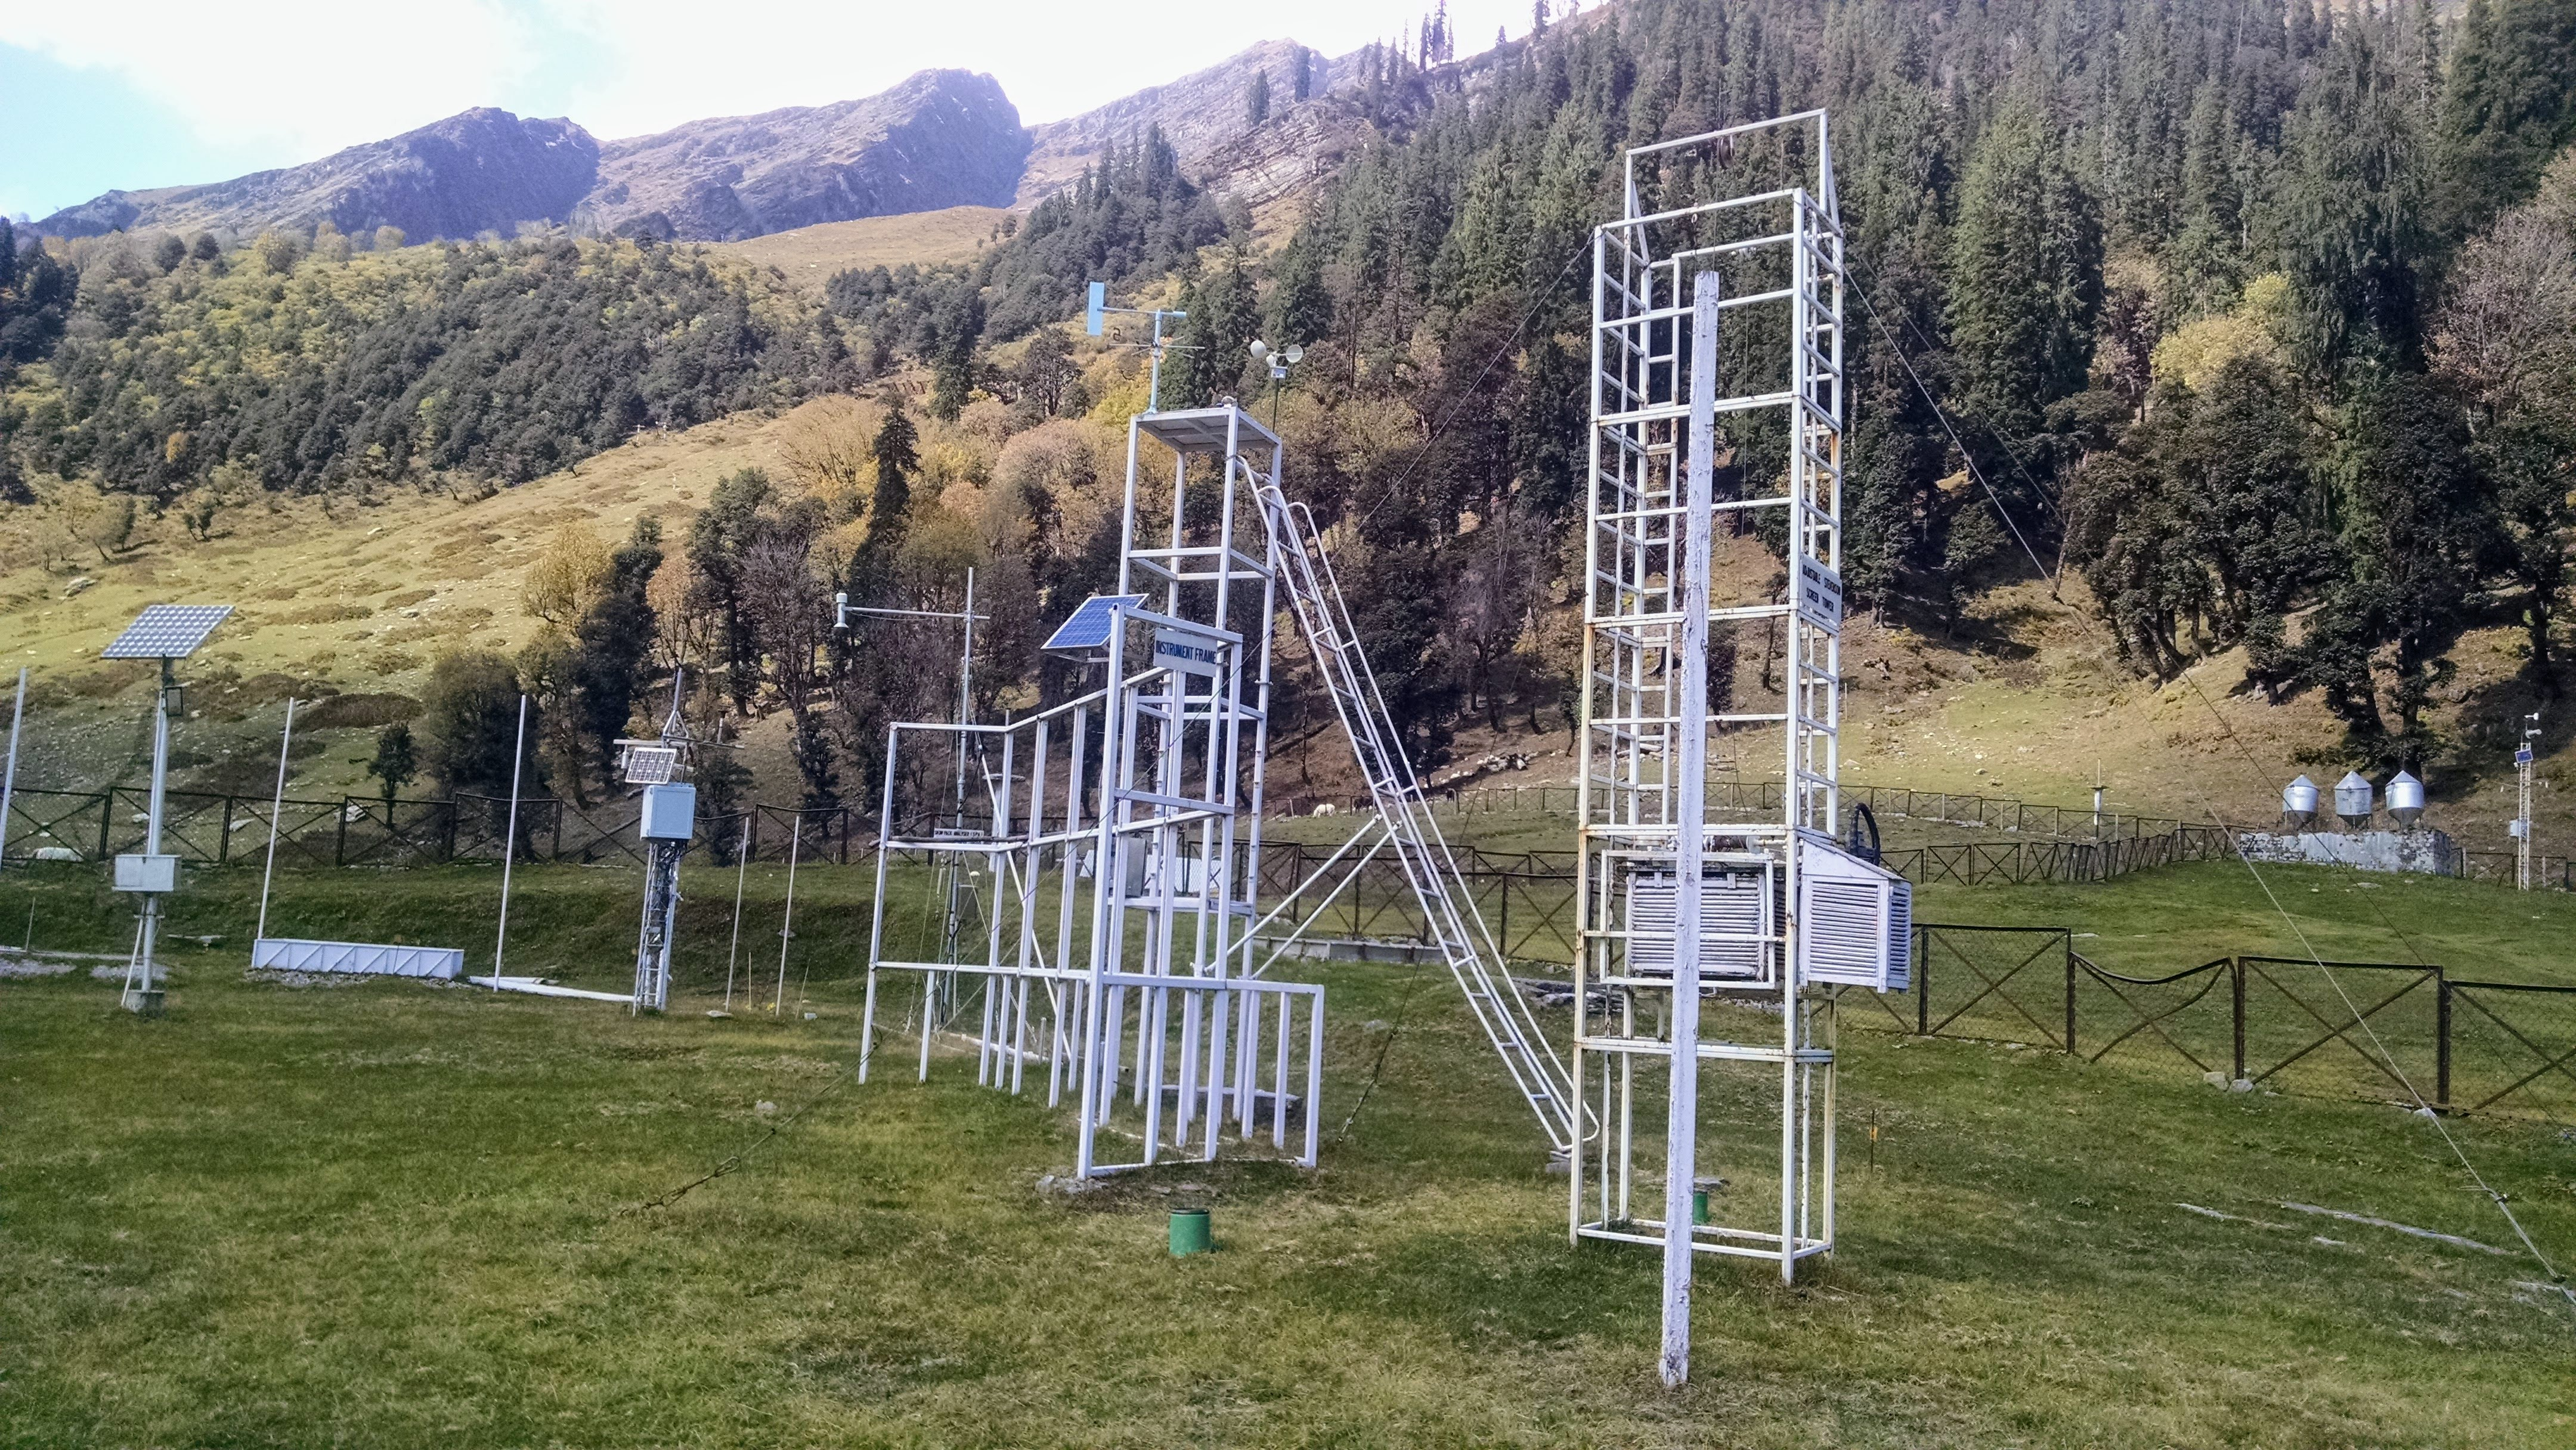
\includegraphics[width=\textwidth]{Figures/Field/stations.jpg}}
        \caption{Weather instruments}
        \label{subfig:stations}
    \end{subfigure}
    \caption{Dhundi field photographs showing the varying topographic features present in the surrounding area.}
    \label{fig:field}
\end{figure}

\begin{table}[!htbp]
\centering
\caption{Bistatic TerraSAR-X/TanDEM-X dataset metadata. The date and time are shown in DD/MM/YYYY and UTC hrs formats respectively.}
\label{table:data}
\begin{tabular}{c c c c c c}
\hline
\textbf{Date}    & \textbf{Time}   & \textbf{Polarisation}   & \textbf{Orbital Direction}    & \boldmath$B_\bot$ (m) & \boldmath$h_{2\pi}$ (m) \\ \hline
29/12/2015  & 12:46 & Quad  & Ascending & 273.51    & 18.54 \\ 
08/01/2016  & 00:53 & Quad  & Descending    & 96.34 & 63.18 \\ 
09/01/2016  & 12:46 & Quad  & Ascending & 288.29    & 17.61 \\ 
19/01/2016  & 00:53 & Quad  & Descending    & 96.10 & 63.34 \\ 
20/01/2016  & 12:46 & Quad  & Ascending & 289.68    & 17.53 \\ 
30/01/2016  & 00:53 & Quad  & Descending    & 98.15 & 62.02 \\ 
06/01/2017  & 12:46 & HH    & Ascending & 230.17    & 22.18 \\ 
24/03/2017  & 12:46 & Dual  & Ascending & 377.97    & 13.44 \\
15/04/2017  & 12:46 & Dual  & Ascending & 327.53    & 15.52 \\
26/04/2017  & 12:46 & Dual  & Ascending  & 286.69   & 17.73 \\
08/06/2017  & 00:53 & Dual  & Descending    & 93.09 & 65.37 \\
24/08/2017  & 00:53 & Dual  & Descending    & 17.51 & 347.49 \\ \hline
\end{tabular}
\end{table}

\subsection{Datasets Used}
\label{ssec:data}
Overall twelve Coregistered Single look Slant range Complex (CoSSC) TerraSAR-X (TSX)/TanDEM-X (TDX) bistatic X-band SAR images acquired between December 2015 and August 2017 in stripmap (SM) mode are available over this study area \citep{Balss2012}. The datasets are summarised in Table \ref{table:data}. In total, there are six Quad-pol data pairs wherein the ascending and descending orbital pass acquisitions are at 12:46 hrs and 00:53 hrs Universal Time Coordinated (UTC) respectively. Moreover, the perpendicular baseline ($B_\bot$) and ambiguity height ($h_{2\pi}$) for these datasets are also provided in \ref{table:data}. 

Additionally, the high frequency data (two-minute interval measurements) obtained from the snowpack analyser (SPA) device (installed at Dhundi) had been downloaded and were added to the database as a separate table. Accordingly, the in-situ SSDs and snow densities at 06:22 hrs (00:52 hrs UTC) and 18:16 hrs (12:46 hrs UTC) Indian Standard Time (IST) for the descending and ascending pass acquisitions respectively have been considered. The in-situ SSDs along with the corresponding snow densities and SSWEs are provided in Table \ref{table:ssd_data}. Apart from this, a forest mask used in previous studies involving this watershed area \citep{Thakur2012, Thakur2017} has been obtained from the Water Resources Department (WRD), Indian Institute of Remote Sensing (IIRS).

\begin{table}[htb]
\centering
\caption{In-situ SSD, snow density, and SSWE measured by the SPA instrument at the Dhundi site. The date and time are in DD/MM/YYYY and UTC hrs respectively.}
\label{table:ssd_data}
\begin{tabular}{c c c c c}
\hline
\textbf{Date}    & \textbf{Time}   & \textbf{SSD (cm)}   & \textbf{Snow Density (g/cm\textsuperscript{3})} & \textbf{SSWE (mm)}  \\ \hline
29/12/2015  & 12:46 & 36.70  & 0.382    & 140.19    \\ 
08/01/2016  & 00:52 & 54.90  & 0.315    & 172.94    \\ 
09/01/2016  & 12:46 & 56.00  & 0.304    & 170.24    \\ 
19/01/2016  & 00:52 & 42.80  & 0.347    & 148.52    \\ 
20/01/2016  & 12:46 & 42.80  & 0.338    & 144.66    \\ 
30/01/2016  & 00:52 & 70.00  & 0.210    & 147.00    \\ \hline
\end{tabular}
\end{table}

The Sentinel Application Platform (SNAP) 7.0.0 \citep{ESA2019} has been used for basic SAR processing. In addition, the FSD and SSD inversion models have been implemented using Python 3 wherein PyCharm Community Edition 2019.3.1 \citep{JetBrains2019} was used as the coding environment. Moreover, the final snow depth maps have been prepared using QGIS 3.10 \citep{QGISDevelopmentTeam2019}. Furthermore, some of the computationally intensive tasks have been carried out using the High-Performance Computing (HPC) infrastructure installed at IIRS.
\FloatBarrier
\section{Results and Discussion}
\label{sec:res}
\subsection{Scattering Mechanisms}
\label{ssec:scat}

The winter (January 8, 2016) and summer-time (June 8, 2017) dual-pol $H/{\alpha}$ decomposition (Figure \ref{fig:ha_res}) and unsupervised Wishart classification (Figure \ref{fig:wishart_res}) results combined with the derived class percentage statistics (Figure \ref{fig:percent}) show that, in the presence of snow, the high entropy anisotropic volume scattering (Z8) increases by 5.11\% whereas the medium entropy volume scattering (Z5) decreases by 7.01\% for the entire study area. This reduction in the Z5 volume scattering could be attributed to the partially snow covered forests and shrubs which exhibit higher volume scattering at X-band during the snow-free season (Figure \ref{subfig:mountain}). The corresponding dual-pol Wishart classified maps are displayed along with the zoomed views in Figure \ref{subfig:wishart_jan} and Figure \ref{subfig:wishart_jun} respectively.

Moreover, the Bragg surface scattering (Z3) is slightly higher in summer (10.88\%) as compared to the winter (10.38\%). One plausible reason for this is the 20 mm rainfall which occurred on June 7, 2017, evening (data retrieved from the Dhundi record book). Also, the occurrence of fresh snowfall in areas which did not have prior standing or old snow could result in surface scattering from the ground \citep{Leinss2014}. Apart from this, the asbestos gable roofs used in the human settlements (Figure \ref{subfig:base} and Figure \ref{subfig:landscape}) are strong single-bounce surface scatterers \citep{Brunner2009}. 

\begin{figure}[!ht]
    \centering
    \begin{subfigure}[t]{\textwidth}
        \raisebox{-\height}{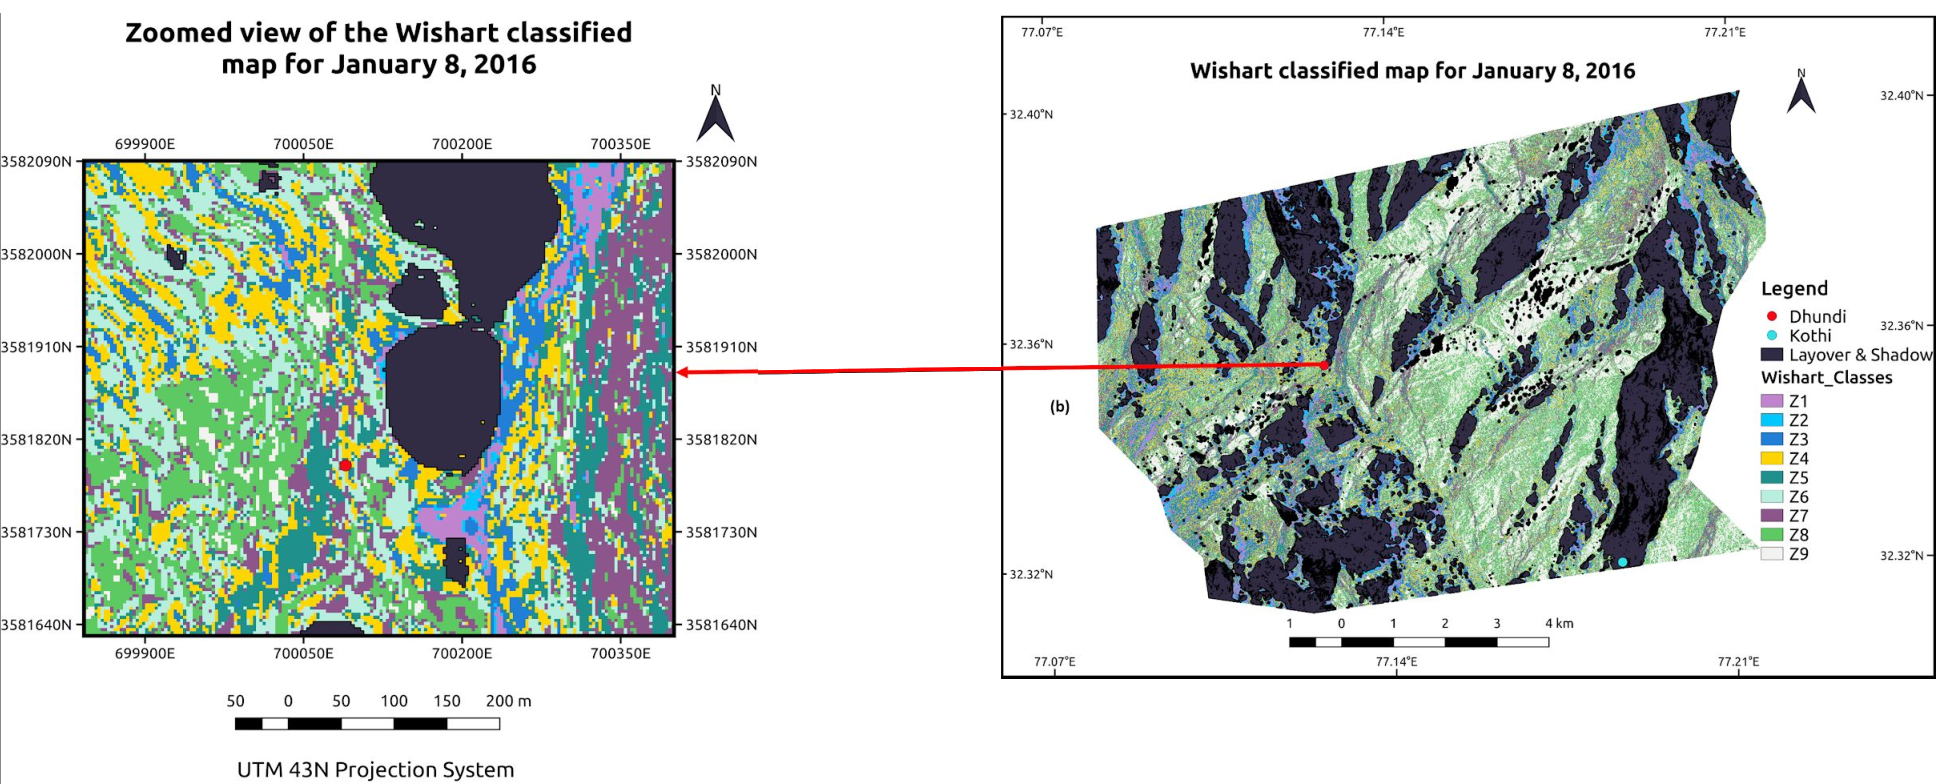
\includegraphics[width=\textwidth]{Figures/Results/wishart_jan.png}}
        \caption{}
        \label{subfig:wishart_jan}
    \end{subfigure}
    %%%%%%%%%%%%%%%%%%%%%%%%%%%%%%%%%%%second row
    \begin{subfigure}[t]{\textwidth}
        \raisebox{-\height}{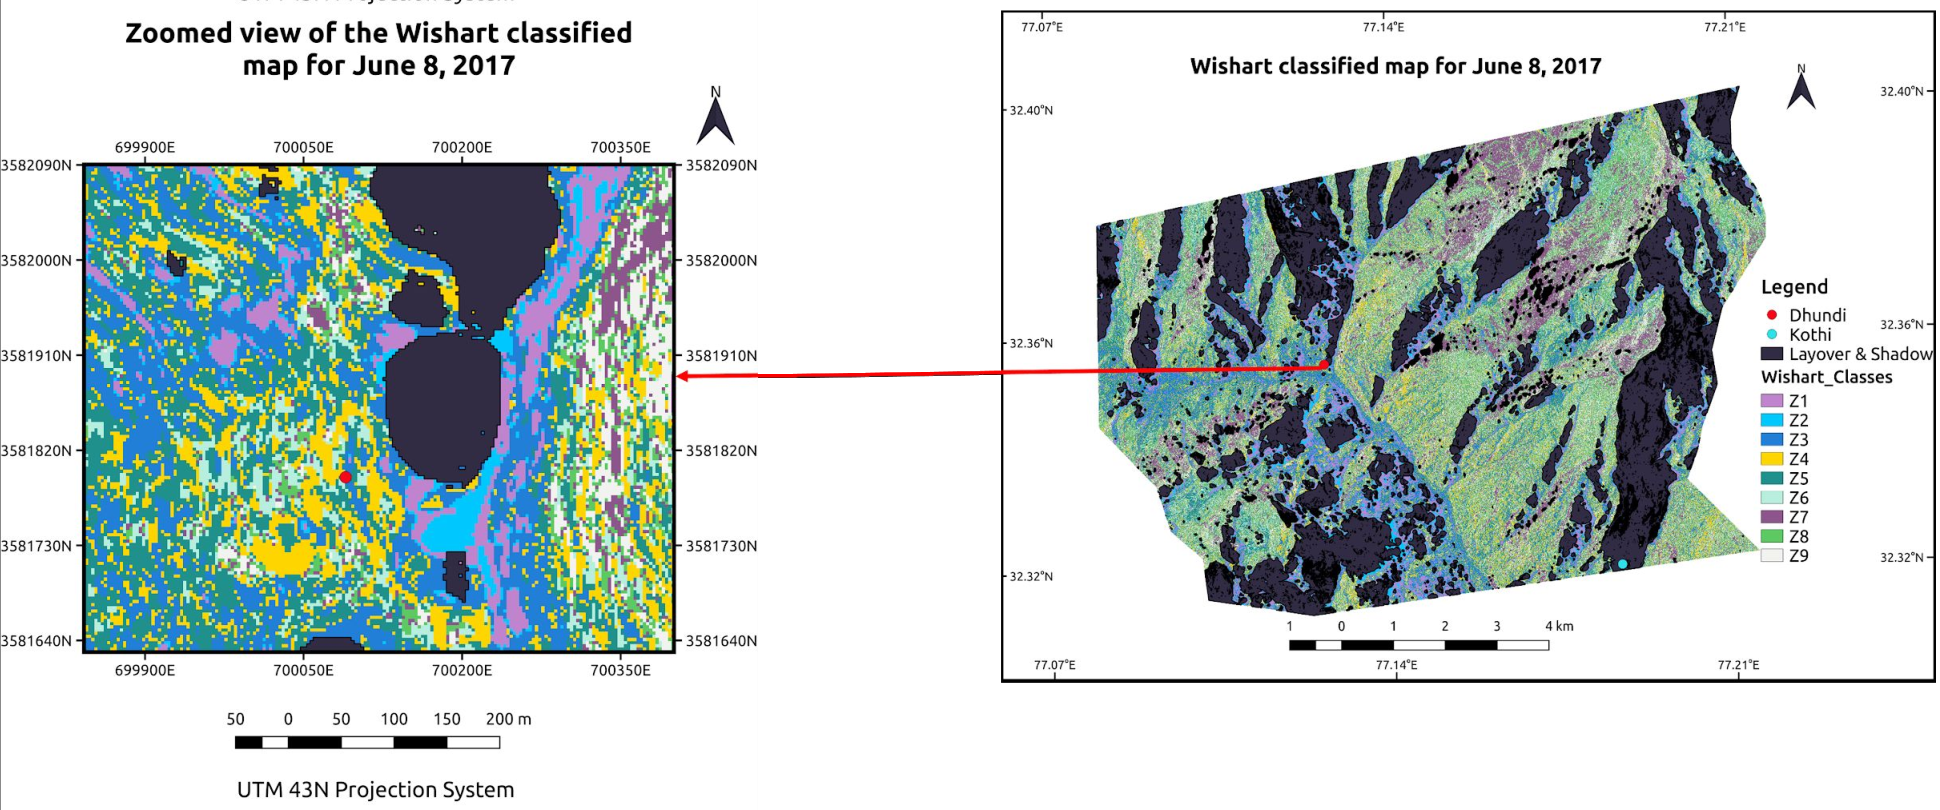
\includegraphics[width=\textwidth]{Figures/Results/wishart_jun.png}}
        \caption{}
        \label{subfig:wishart_jun}
    \end{subfigure}
    \caption{Zoomed views over Dhundi of the Wishart classified maps for the \subref{subfig:wishart_jan} January 8, 2016, and \subref{subfig:wishart_jun} June 8, 2017 data. In these maps, only the layover and shadow mask has been applied. Also, the Kothi area is excluded from the analysis since it lies in the layover region.}
    \label{fig:wishart_res}
\end{figure}

However, with snow accumulation on these materials, the surface scattering could be reduced. Another prominent feature noticeable in Figure \ref{subfig:wishart_jun} is the high amount of surface scattering from the river bed (Figure \ref{subfig:beas}) during the summer season. This is caused by both the boulders and the increasing flow of snow-melt water in the river (Figure \ref{subfig:beas}).

Furthermore, the human settlements result in double-bounce scattering (Z4) \citep{Brunner2009}, which in the winter-time scenario reduces by 0.34\%. Also, the random surface scattering (Z6) increases by 0.66\% which could be caused by the presence of small snow patches on the ground. Other than this, there is a strong decrease in the low entropy multiple (dihedral) scattering from 8.23\% to 5.17\% in the snow-covered season which could be caused by the added snow layer on the buildings and also boulders.

\begin{figure}[htb]
    \centering
    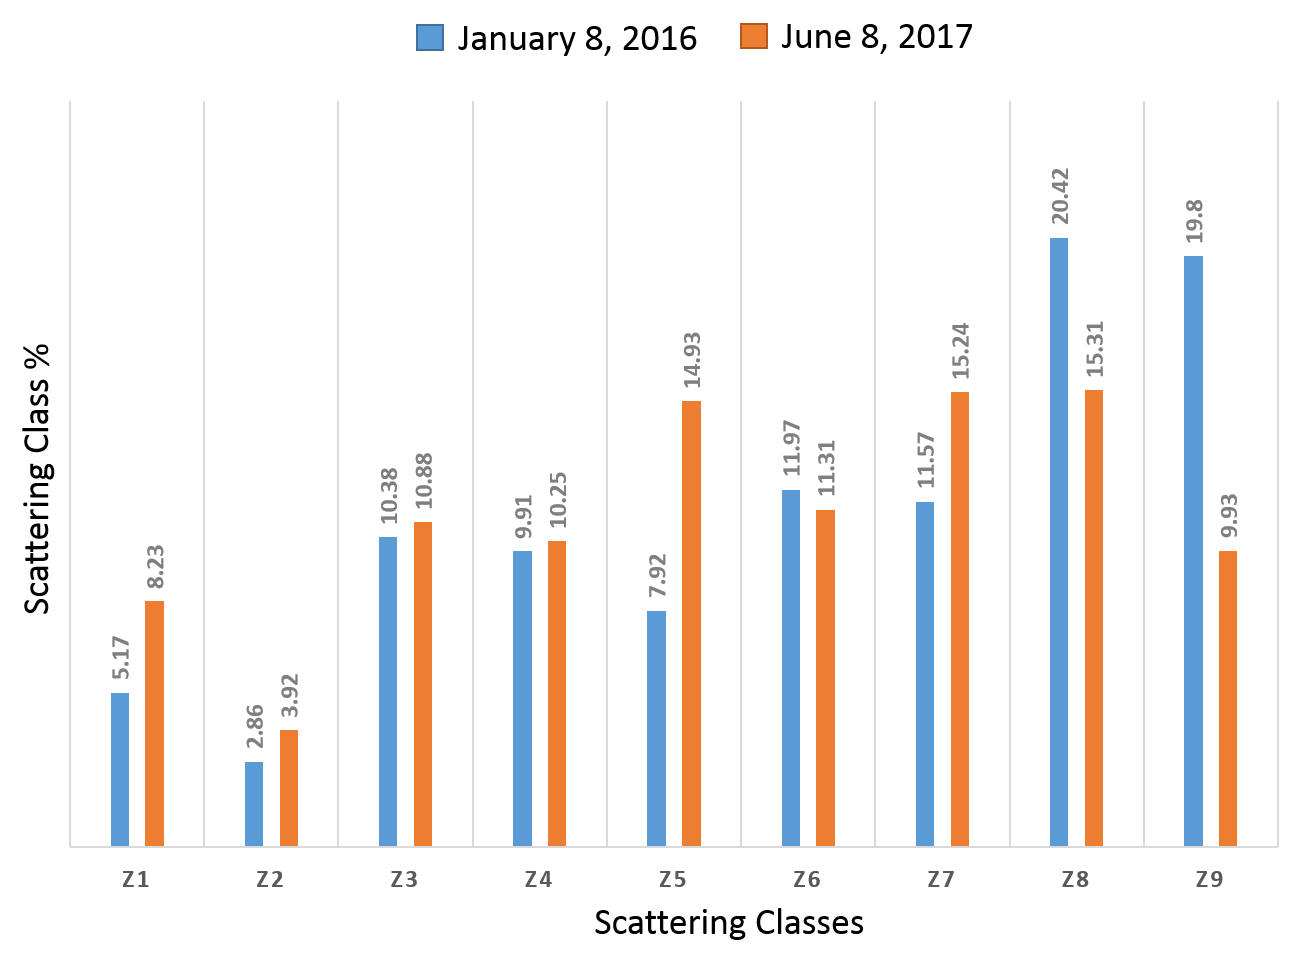
\includegraphics[width=\textwidth]{Figures/Results/Percent.png}
    \caption{Scattering class percentages (rounded to 2 decimal places) from the unsupervised Wishart classification. The different zone labels are described in Figure \ref{fig:ha}.}
    \label{fig:percent}
\end{figure}

Another interesting aspect in this context is the increase (from 9.93\% to 19.8\%) in the number of unclassified or non-feasible pixels (Z9) for the winter-time image (Figure \ref{fig:percent}) which is also depicted through the $H/{\alpha}$ plane plots in Figure \ref{subfig:ha_jan} and Figure \ref{subfig:ha_jun}. This is primarily resulting from the added terrain complexity owing to the snow accumulation. In order to resolve this issue, the quad-pol entropy ($H$), anisotropy ($A \in$ [0, 1]), alpha ($\alpha$), $H/A/{\alpha}$ decomposition has been applied on the January 8, 2016 data. The corresponding $H/{\alpha}$ plane plot in Figure \ref{subfig:ha_jan_quad} shows that the quad-pol approach is able to fully classify the winter-time image. However, since the summer-time image is having only HH and VV channels, the dual-pol method has been used to properly compare the respective scattering mechanisms \citep{Majumdar2019}.

\begin{figure}[htb]
    \centering
    \begin{subfigure}[t]{0.49\textwidth}
        \raisebox{-\height}{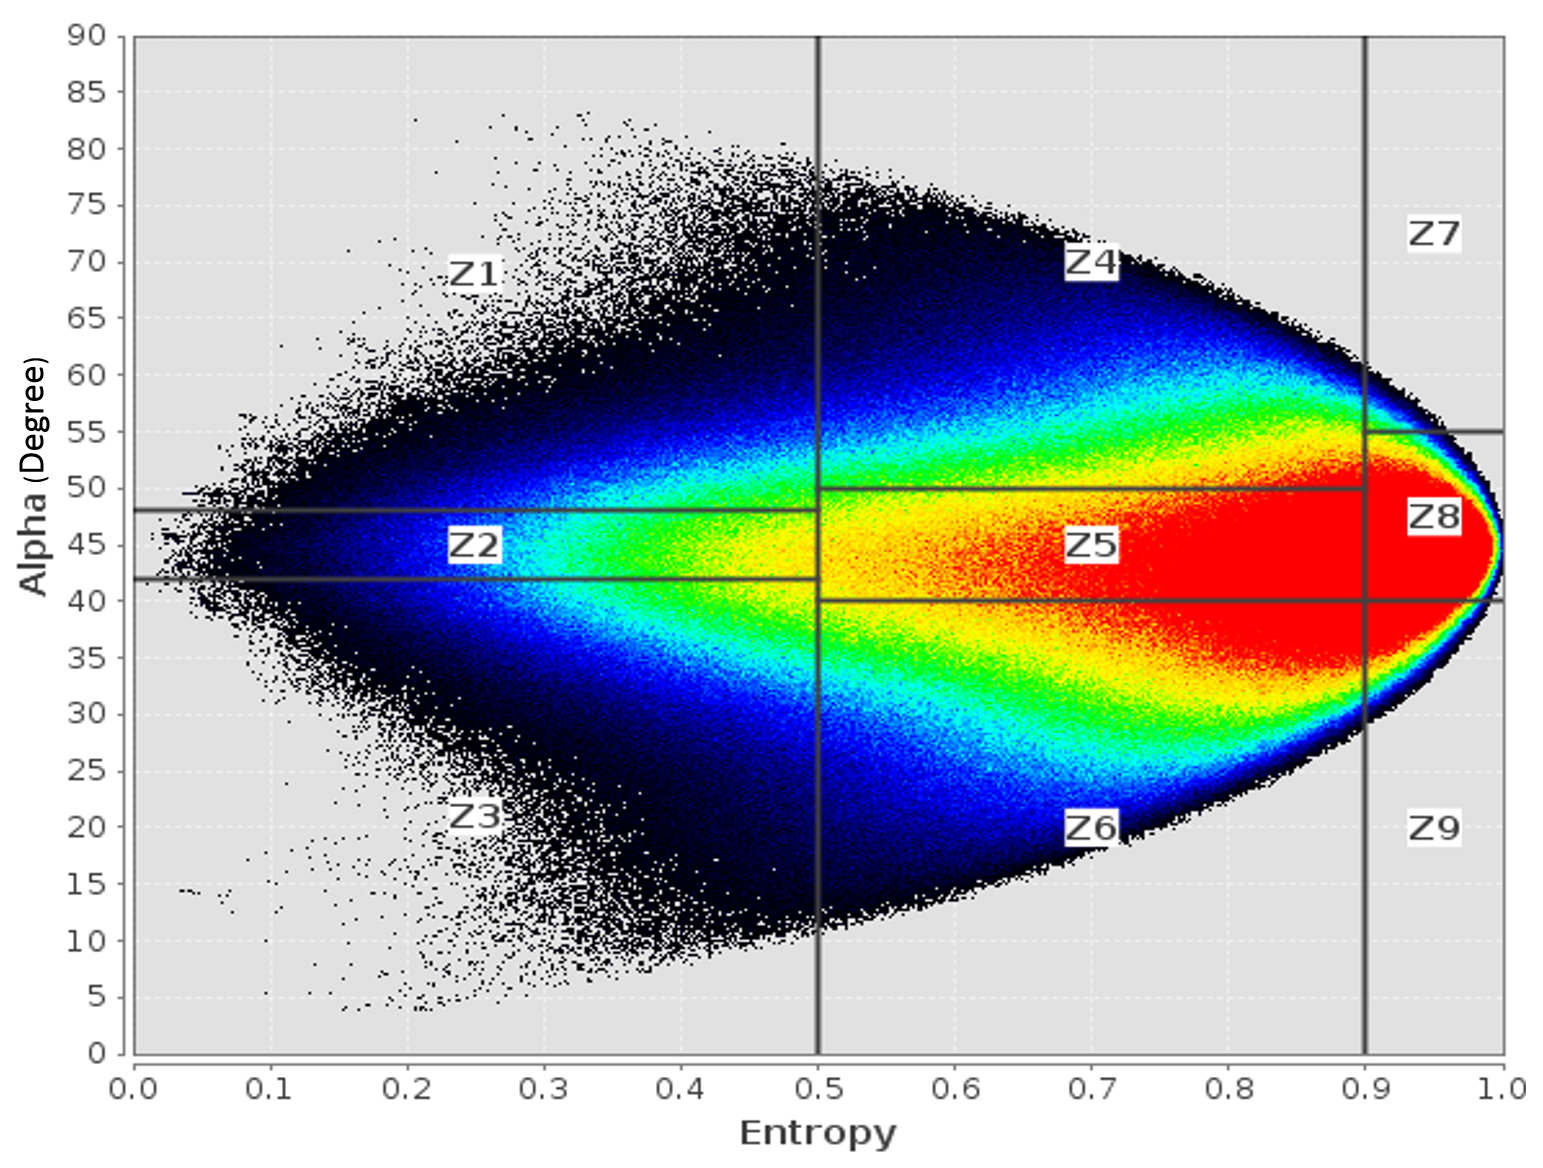
\includegraphics[width=\textwidth]{Figures/Results/ha_jan.png}}
        \caption{}
        \label{subfig:ha_jan}
    \end{subfigure}
    \hfill
    \begin{subfigure}[t]{0.49\textwidth}
        \raisebox{-\height}{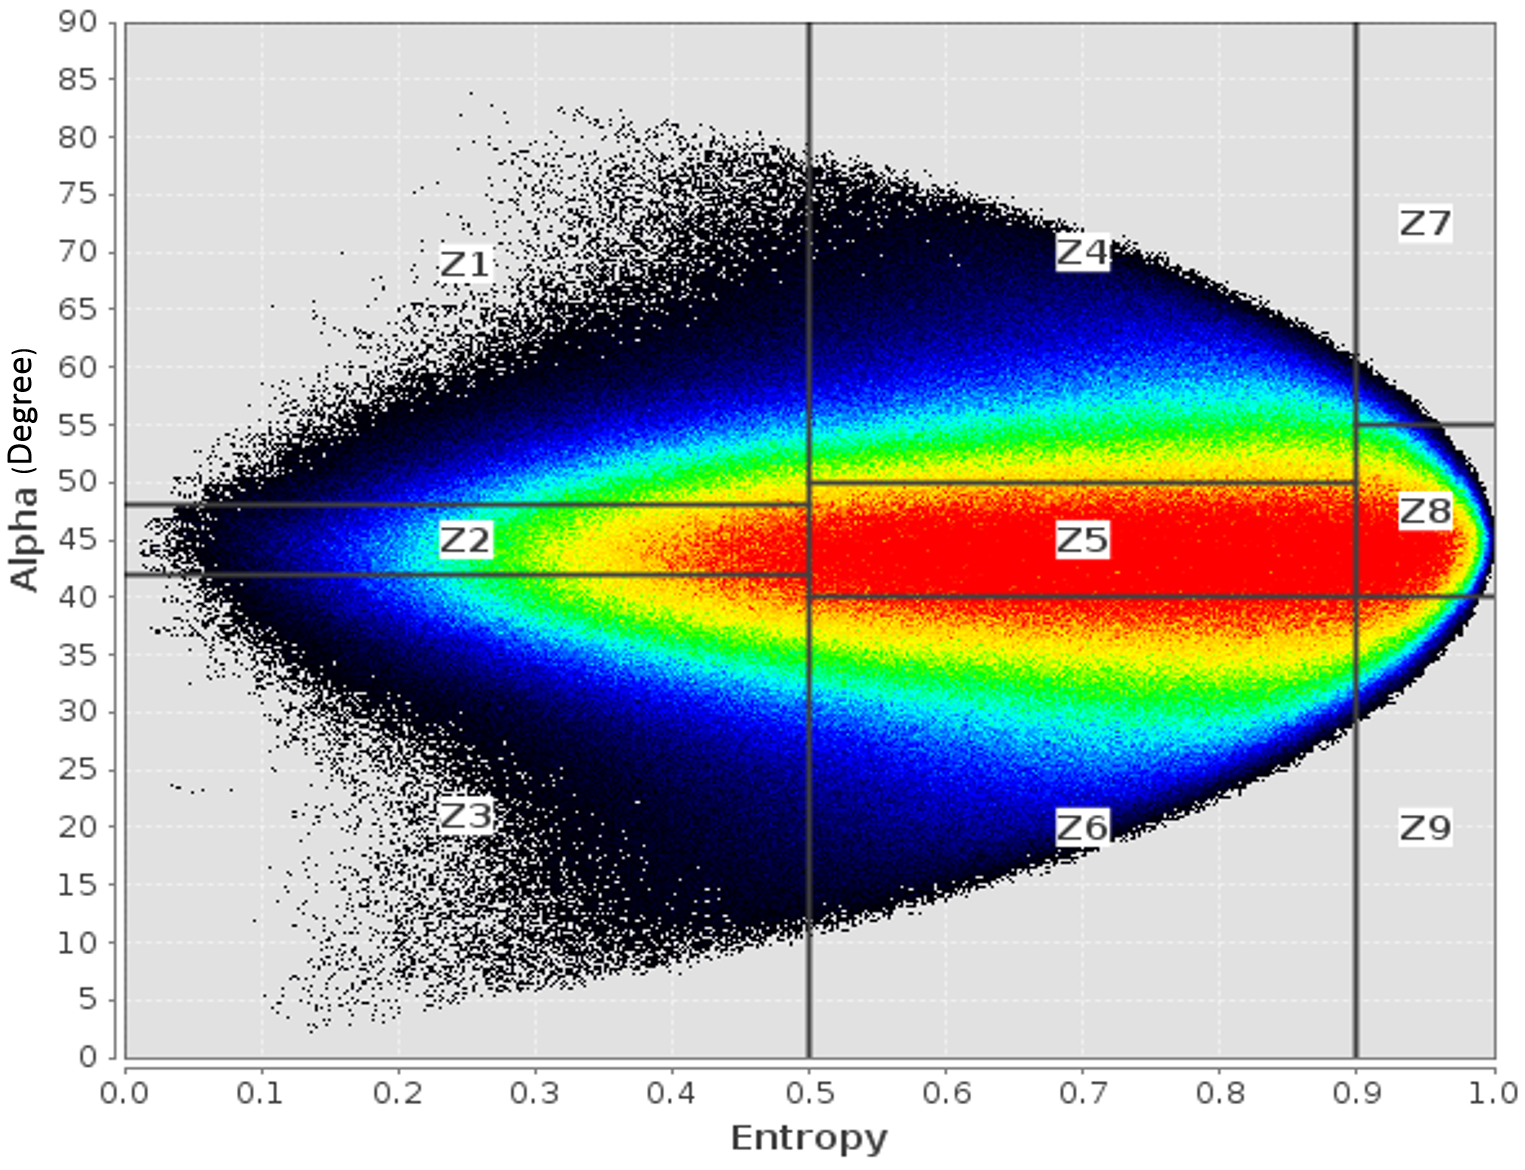
\includegraphics[width=\textwidth]{Figures/Results/ha_jun.png}}
        \caption{}
        \label{subfig:ha_jun}
    \end{subfigure}
    %%%%%%%%%%%%%%%%%%%%%%%%%%%%%%%%%%%second row
    \begin{subfigure}[t]{0.49\textwidth}
        \raisebox{-\height}{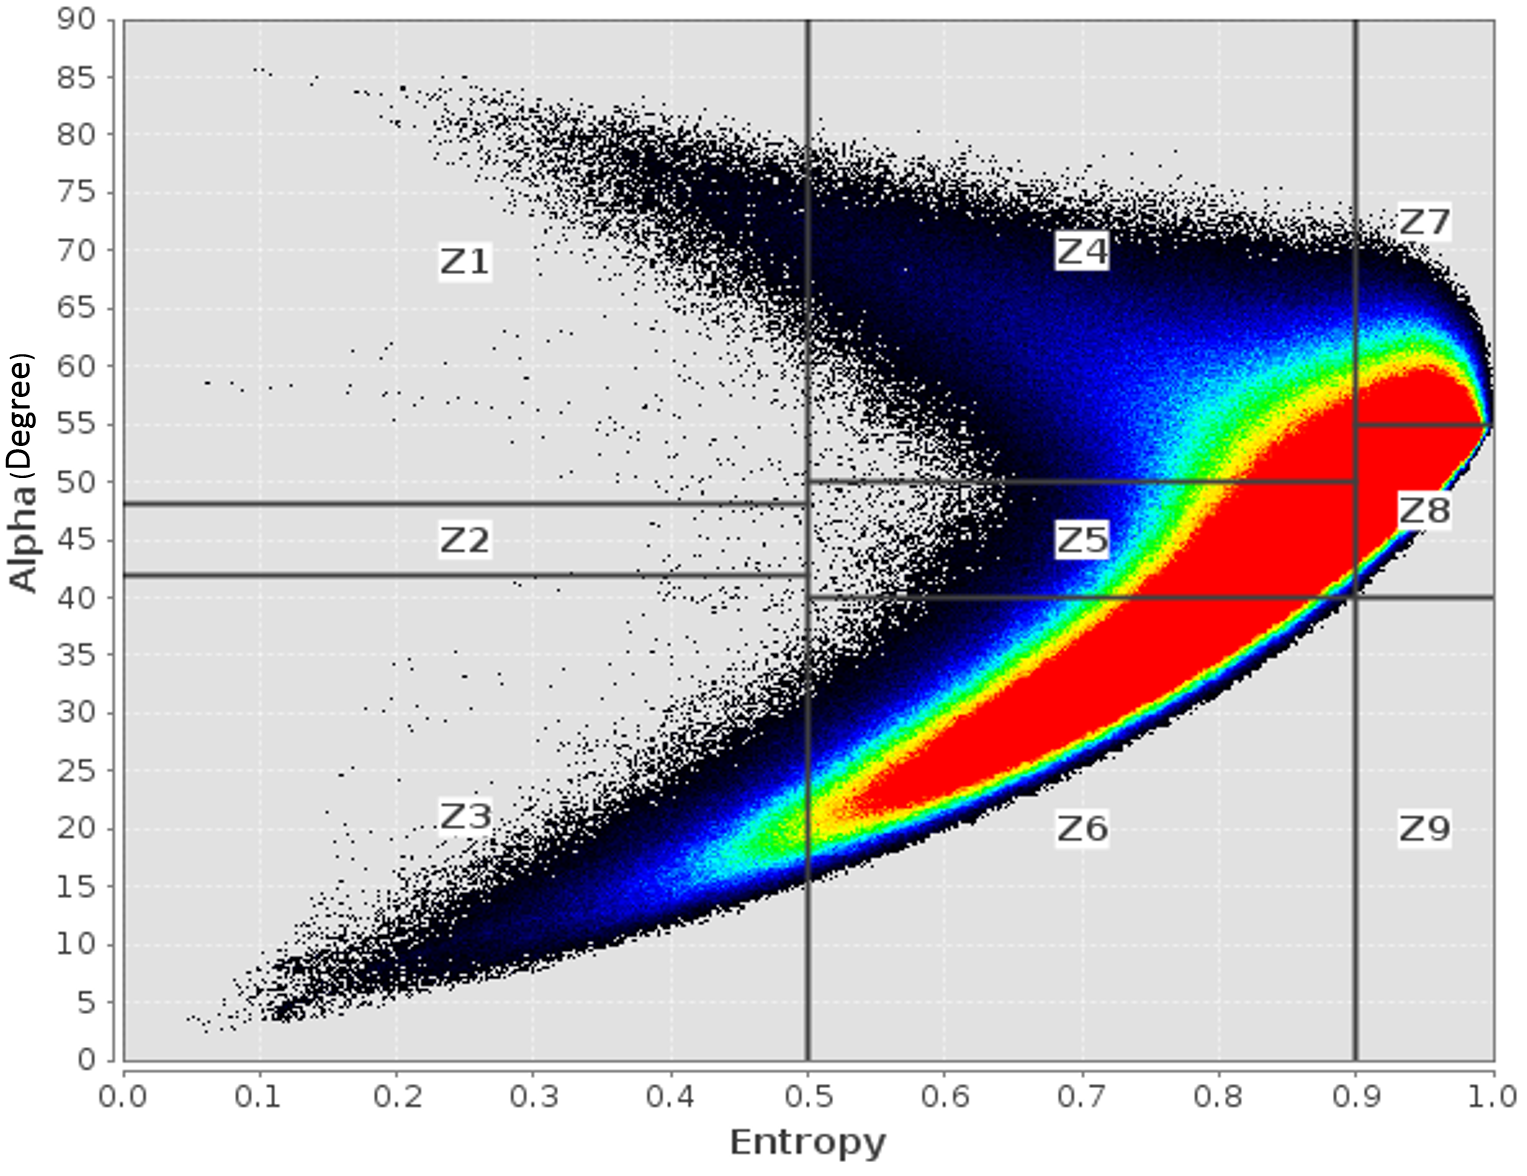
\includegraphics[width=\textwidth]{Figures/Results/ha_jan_quad.png}}
        \caption{}
        \label{subfig:ha_jan_quad}
    \end{subfigure}
    \caption{Dual-pol $H/{\alpha}$ plane plots for the \subref{subfig:ha_jan} January 8, 2016, and \subref{subfig:ha_jun} June 8, 2017 data, \subref{subfig:ha_jan_quad} Quad-pol $H/{\alpha}$ plane plot for the January 8, 2016 data. The colours red, green, blue, and black indicate the point density with red being the highest, and black as the lowest. These plots have been made using SNAP \citep{ESA2019}.}
    \label{fig:ha_res}
\end{figure}

Thus, from this discussion, it is clearly observed that the presence of snow causes a substantial change of the scattering patterns in the study area resulting in significant uncertainty sources. In turn, the optimisation of the model parameters along with the sensitivity analysis of the SSD values depend on these scattering types. As an example, if there is low surface scattering then the FSD inversion model leads to underestimated values \citep{Leinss2014} whereas for low volume scattering, the SSD results are generally underestimated \citep{Cloude2005, Hajnsek2009, Kugler2015}. Therefore, the uncertainty assessment by means of the scattering mechanism classification is one of the key aspects of this research.
\FloatBarrier
\subsection{Changes in Surface Coherence}
The summer (June 8, 2017) and winter (January 8, 2016) surface coherences are compared in Fig \ref{fig:coh_res} which indicate higher surface coherence values for the summer time image (Fig \ref{subfig:coh_jun}). These surface coherences are computed only from the VV channel using standard InSAR workflow in SNAP \citep{ESA2019}. The visual analysis suggests that the surface coherence is higher (implying higher surface scattering) during June 8, 2017 which is in concordance with the backscattering mechanisms discussed in the previous section (Fig \ref{fig:wishart_res}). Accordingly, the mean surface coherence (calculated using the 3$\times$3 window in Dhundi) is reduced from $\sim0.83$ to $\sim0.78$ during the winter time (Fig \ref{subfig:coh_jan}) due to the presence of standing snow. However, this reduction is small owing to the occurrence of fresh snowfall on January 8, 2016 which results in surface scattering at X-band \citep{Leinss2014}. 

\begin{figure}[!ht]
    \centering
    \begin{subfigure}[t]{\textwidth}
        \raisebox{-\height}{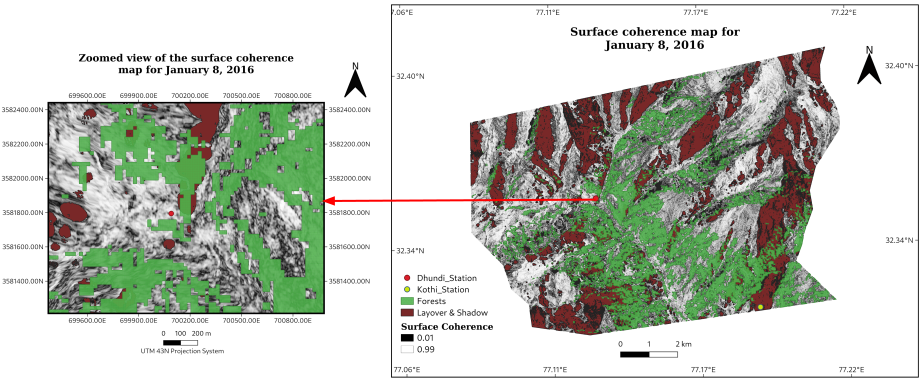
\includegraphics[width=\textwidth]{Figures/Results/Coh_Maps_01082016.png}}
        \caption{}
        \label{subfig:coh_jan}
    \end{subfigure}
    %%%%%%%%%%%%%%%%%%%%%%%%%%%%%%%%%%%second row
    \begin{subfigure}[t]{\textwidth}
        \raisebox{-\height}{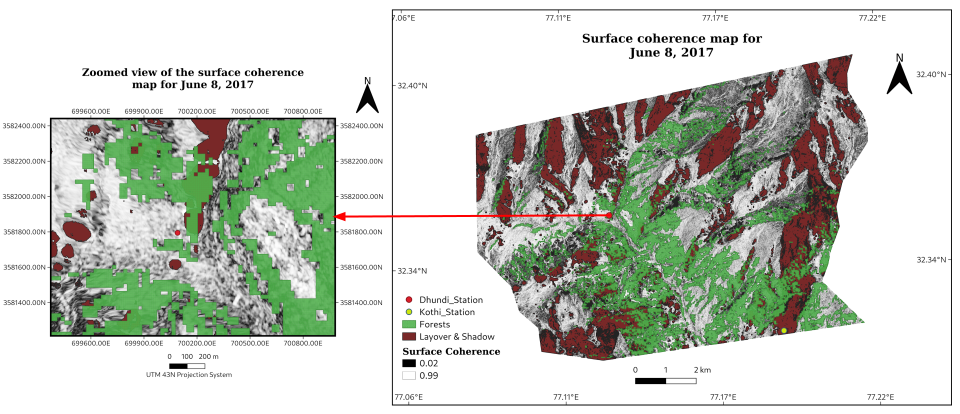
\includegraphics[width=\textwidth]{Figures/Results/Coh_Maps_06082017.png}}
        \caption{}
        \label{subfig:coh_jun}
    \end{subfigure}
    \caption{Zoomed views over Dhundi of the surface coherence maps for the \subref{subfig:coh_jan} January 8, 2016, and \subref{subfig:coh_jun} June 8, 2017 data.}
    \label{fig:coh_res}
\end{figure}
\FloatBarrier
\subsection{Sensitivity Analysis Results}
\label{ssec:sar}
In order to perform the sensitivity analysis, only the Dhundi area is chosen and the January 8, 2016 acquisition is used for this purpose. Accordingly, the other datasets have been tested for the overall accuracy assessment based on the optimised parameters for the January 8, 2016 data.

The SSD inversion model as described from the implementation or methodological perspective in section \ref{ssec:ssd} incorporates several user-defined free parameters. Thus, it is necessary to conduct an appropriate sensitivity analysis for the hybrid Pol-InSAR based volumetric height (SSD) retrieval algorithm. Accordingly, the various model parameters and their optimisation are discussed below.

\subsubsection{Volume and Surface Coherence Ensemble Window}

The ensemble windows corresponding to the number of looks (L) in Eq. \eqref{seq:coh} must be suitably chosen so as to maximise both the volume coherence amplitude, $\gamma\left(\vv{w_v}\right)$, and the surface coherence amplitude, $\gamma\left(\vv{w_s}\right)$. As a result, the sensitivity analysis for these window sizes is an important aspect of this work.

The effects of $L$ on the mean volume coherence amplitude, $\mu_{\gamma\left(\vv{w_v}\right)}$ and the mean surface coherence amplitude, $\mu_{\gamma\left(\vv{w_s}\right)}$ which are measured by applying the same 3$\times$3 neighbourhood window over Dhundi (section \ref{ssec:ssd}) along with the respective standard deviations, $\sigma_{\gamma\left(\vv{w_v}\right)}$ and $\sigma_{\gamma\left(\vv{w_v}\right)}$, are displayed in Figure \ref{fig:ssd_coh}. 

\begin{figure}[htb]
    \centering
    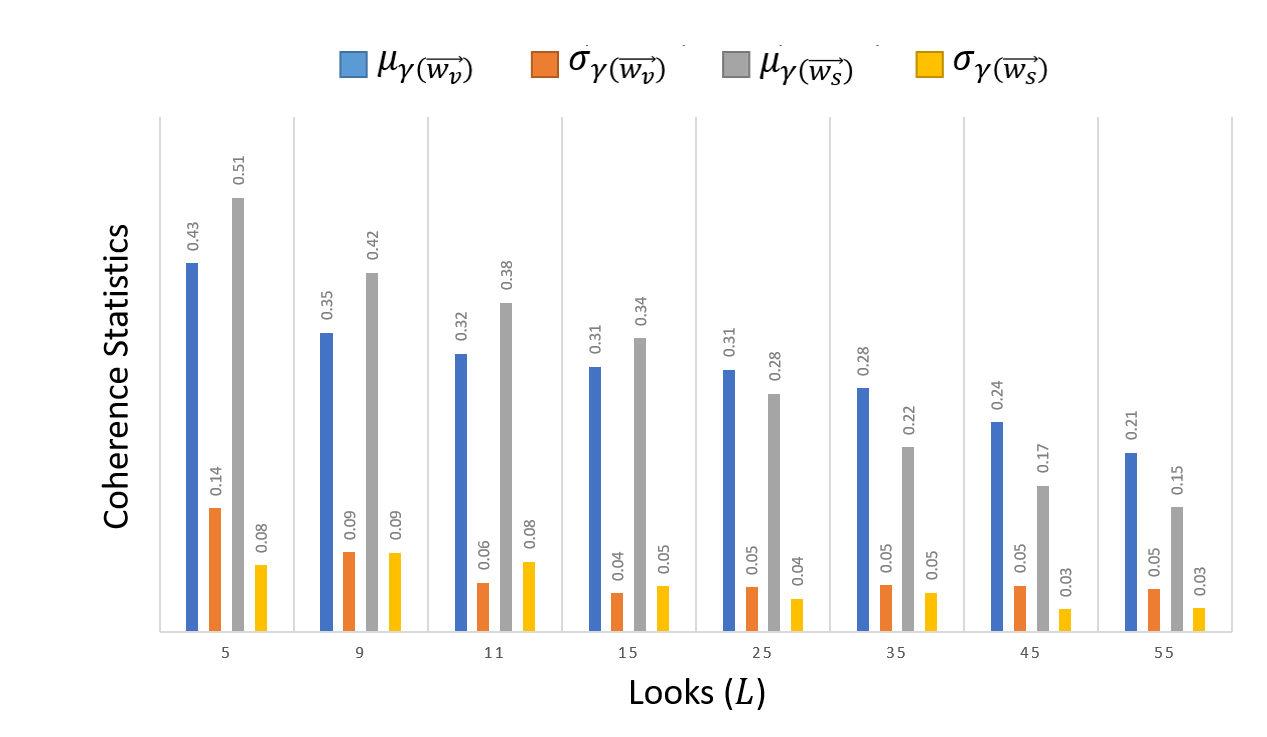
\includegraphics[width=\textwidth]{Figures/Results/Coh_SSD.png}
    \caption{Effect of the number of looks ($L$) on the volume and surface coherence. All the values are rounded to 2
decimal places.}
    \label{fig:ssd_coh}
\end{figure}

It can be seen that for the executed test cases, with increasing $L$, there is a general decreasing trend for both these coherences. So, for the SSD estimation, $L =$ 3 is chosen even though \cite{Cloude2005} suggests the usage of higher values of $L$. This is because, $\sigma_{\gamma\left(\vv{w_v}\right)} \approx$ 0.1 and $\sigma_{\gamma\left(\vv{w_s}\right)} \approx$ 0.18 are sufficiently small with adequately high $\mu_{\gamma\left(\vv{w_v}\right)} \approx$ 0.67 and $\mu_{\gamma\left(\vv{w_s}\right)} \approx$ 0.68. Also, since there is only one validation point for the entire study area, $L =$ 3 is justifiable.

However, there exist several free parameters in this Pol-InSAR based SSD inversion model (section \ref{ssec:ssd}) and hence, the volume and surface coherence ensemble windows need to be kept constant ($L =$ 3) for the subsequent sensitivity analyses of the other parameters.

\subsubsection{Scaling Parameters}
\label{sssec:scale}
It has been previously discussed in section \ref{ssec:ssd} that there are two scaling parameters involved in the SSD estimation process. These are the vertical wavenumber scaling parameter ($\eta^\prime\in\mathbb{R}_{>0}^+$) and the scaling factor ($\eta\in$ [0, 1]) of the hybrid DEM differencing approach developed by \cite{Cloude2010}. More specifically, $\eta^\prime =$ 5 was found suitable for each descending pass acquisitions (Table \ref{table:data}). However, for the December 29, 2015 acquisition, $\eta^\prime =$ 40 because $k_z \approx$ 0.01 rad/m for this dataset was very low as compared to the other datasets ($k_z \approx$ 0.1 rad/m). Similarly, for the January 9, 2016 and January 20, 2016 datasets, $\eta^\prime =$ 3 and $\eta^\prime =$ 4 respectively were found to produce accurate results. Also, the volume coherence threshold, $\tau_v = $ 0.6, $L =$ 3, ground phase median ensemble filter window (21$\times$21), vertical wavenumber ensemble average window (21$\times$21), and the SSD ensemble average window of size 57$\times$57 are unchanged during this sensitivity analysis. So, only $\eta$ is optimised considering the January 8, 2016 data as before.

The monotonically increasing SSD with respect to increasing $\eta$ are displayed in Figure \ref{fig:eta}. For $\eta =$ 0, the standard DEM differencing technique \citep{Cloude2005} results in the mean SSD, $\mu_s \approx$ 42.46 cm with the corresponding SSD standard deviation, $\sigma_s \approx$ 0.49 cm. As the SPA measured SSD at 00:52 hrs UTC, January 8, 2016, is 54.90 cm (Table \ref{table:ssd_data}), so $\mu_s$ is underestimated. Naturally, the mean SSWE, $\mu_{ss} \approx$ 133.76 mm (with SSWE standard deviation, $\sigma_{ss} \approx$ 1.53 mm) is also lower compared to the SPA measured SSWE of 173 mm. Thus, to effectively optimise the SSD, $\eta$ needs to be suitably increased \citep{Cloude2005, Cloude2010}.

\begin{figure}[htb]
    \centering
    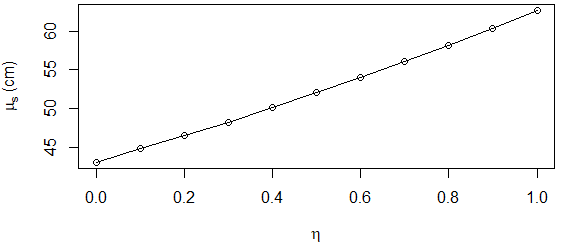
\includegraphics[width=\textwidth]{Figures/Results/Eta.png}
    \caption{Increasing mean SSD with respect to the scaling parameter $\eta$.}
    \label{fig:eta}
\end{figure}

In this context, \cite{Cloude2005} has suggested setting $\eta = $ 0.4 for which the accuracy of the estimated tree height is found to be more than 90\%. Although by keeping $\eta = $ 0.4, $\mu_s \approx$ 49.64 cm ($\sigma_s \approx$ 0.54 cm) is obtained with $\sim$90.42\% accuracy, the complexity of the snow microstructure, anisotropy, and length scales necessitates the need for achieving even higher accuracies \citep{Leinss2016}. Moreover, in the presence of significantly varying hydrometeorological conditions which include high surface roughness and associated uncertainty sources (section \ref{ssec:scat}), the volume and surface coherence amplitudes generally do not reach expected values of higher than 0.8 \citep{Cloude2005, Kugler2015}. Therefore, with $\eta = $ 0.65, the best SSD and SSWE accuracies of 99.53\% ($\mu_s \approx$ 54.64 cm) and 99.48\% ($\mu_{ss} \approx$ 172.10 mm) respectively are achieved over Dhundi (for January 8, 2016) with low standard deviations ($\sigma_s \approx$ 0.58 cm, $\sigma_{ss} \approx$ 1.82 mm) accounting for high reliability. Intriguingly, this model performs sufficiently well for all the six datasets wherein only $\eta^\prime$ needed to be varied for the ascending pass datasets only (section \ref{ssec:snow}). Therefore, these results highlight the significance of this scaling parameter $\eta$ towards controlling the snow structural height variations \citep{Cloude2005, Cloude2010} and hence, the robustness of the hybrid DEM differencing model (section \ref{ssec:ssd}) is verified.

\subsubsection[Computing SINC Inverse]{Computing $\sinc$ Inverse}
\label{sssec:sinc}
In order to test the accuracy of the $\sinc_\pi$ inverse function, sample test data representing the actual inverse, $\alpha_r$, have been prepared as shown in Table \ref{table:2}. Next, the $\sinc_\pi$ of these data, $\sinc_{\pi}\left(\alpha_r\right)$, is computed which essentially corresponds to the possible $\gamma\left(\vv{w_v}\right)$ values. So, the idea of performing sensitivity analysis in this scenario is to check the accuracy of the calculated $\sinc_{\pi_C}^{-1}$ (Eq. \eqref{seq:ncloude}) and $\sinc_{\pi_S}^{-1}$ (Eq. \eqref{seq:secant}) of the $\sinc_{\pi}\left(\alpha_r\right)$ values by comparing these with $\alpha_r$.

\begin{table}[ht]
\centering
\caption{Comparison between the normalised \cite{Cloude2010} sinc inverse and the secant sinc inverse methods.}
\label{table:2}
\begin{tabular}{c c c c}
\hline
\boldmath$\alpha_r$ \textbf{(rad)} & \boldmath$\sinc_{\pi}\left(\alpha_r\right)$   & \boldmath$\sinc_{\pi_C}^{-1}$ \textbf{(rad)}     & \boldmath$\sinc_{\pi_S}^{-1}$ \textbf{(rad)} \\ \hline
0.1                 & 0.984            & 0.103          & 0.100  \\ 
0.2                 & 0.935            & 0.206          & 0.200  \\ 
0.3                 & 0.858            & 0.308          & 0.300  \\ 
0.4                 & 0.757            & 0.409          & 0.400  \\ 
0.5                 & 0.637            & 0.509          & 0.500   \\ 
0.6                 & 0.505            & 0.607          & 0.600  \\ 
0.7                 & 0.368            & 0.703          & 0.700   \\ 
0.8                 & 0.234            & 0.798          & 0.800 \\ 
0.9                 & 0.109            & 0.891          & 0.900 \\ \hline

\end{tabular}
\end{table}

From Table \ref{table:2} it is observed that the secant method converges exactly (up to 13 decimal places) to the
actual $\alpha_r$ while the normalised \cite{Cloude2010} approximation of the $\sinc_\pi$ inverse has some minute errors
involved (RMSE $\approx$ 0.02 rad). Similarly, the $\sinc$ function is tested (Table \ref{table:3}) where $\sinc_C^{-1}$ and $\sinc_S^{-1}$ denote the standard \cite{Cloude2010} approximation (Eq. \eqref{seq:un_cloude}) and the secant method of root finding for the traditional $\sinc$ function respectively. Again, the secant method exactly converges (up to 13 decimal places) whereas RMSE $\approx$ 0.02 rad is associated with the $\sinc_C^{-1}$. The computed results shown in Table \ref{table:2} and Table \ref{table:3} are rounded to 3 decimal places.

\begin{table}[ht]
\centering
\caption{Comparison between the traditional \cite{Cloude2010} sinc inverse and the secant sinc inverse methods.}
\label{table:3}
\begin{tabular}{c c c c}
\hline
\boldmath$\alpha_r$ \textbf{(rad)} & \boldmath$\sinc\left(\alpha_r\right)$   & \boldmath$\sinc_C^{-1}$ \textbf{(rad)}     & \boldmath$\sinc_S^{-1}$ \textbf{(rad)} \\ \hline
0.1                 & 0.998            & 0.103          & 0.100  \\ 
0.2                 & 0.993            & 0.207          & 0.200  \\ 
0.3                 & 0.985            & 0.310          & 0.300  \\ 
0.4                 & 0.974            & 0.413          & 0.400  \\ 
0.5                 & 0.959            & 0.516          & 0.500   \\ 
0.6                 & 0.941            & 0.618          & 0.600  \\ 
0.7                 & 0.920            & 0.721          & 0.700   \\ 
0.8                 & 0.897            & 0.823          & 0.800 \\ 
0.9                 & 0.870            & 0.925          & 0.900 \\ \hline

\end{tabular}
\end{table}

Therefore, by performing the sensitivity analysis of the $\sinc_{\pi_C}^{-1}$, $\sinc_{\pi_S}^{-1}$, $\sinc_C^{-1}$, and $\sinc_S^{-1}$, it is clearly understood that the secant method provides highly accurate results. Hence, in this work, $\sinc_{\pi_S}^{-1}$ is applied for solving Eq. \eqref{seq:hybrid_dem} wherein the $\sinc_{\pi_C}^{-1}\left(\gamma\left(\vv{w_v}\right)\right)$ value is used as an initial guess to the secant method for faster convergence.

\subsubsection{SSD Ensemble Window}

Another essential free parameter used in the Pol-InSAR based SSD estimation model (section \ref{ssec:ssd}) is the SSD ensemble averaging window size. By keeping $\eta = $ 0.65, $\eta^\prime = $ 5, and other ensemble window sizes constant, the sensitivity analysis has been carried out to observe the SSD variations which are shown in Figure \ref{fig:swindow}. 

\begin{figure}[htb]
    \centering
    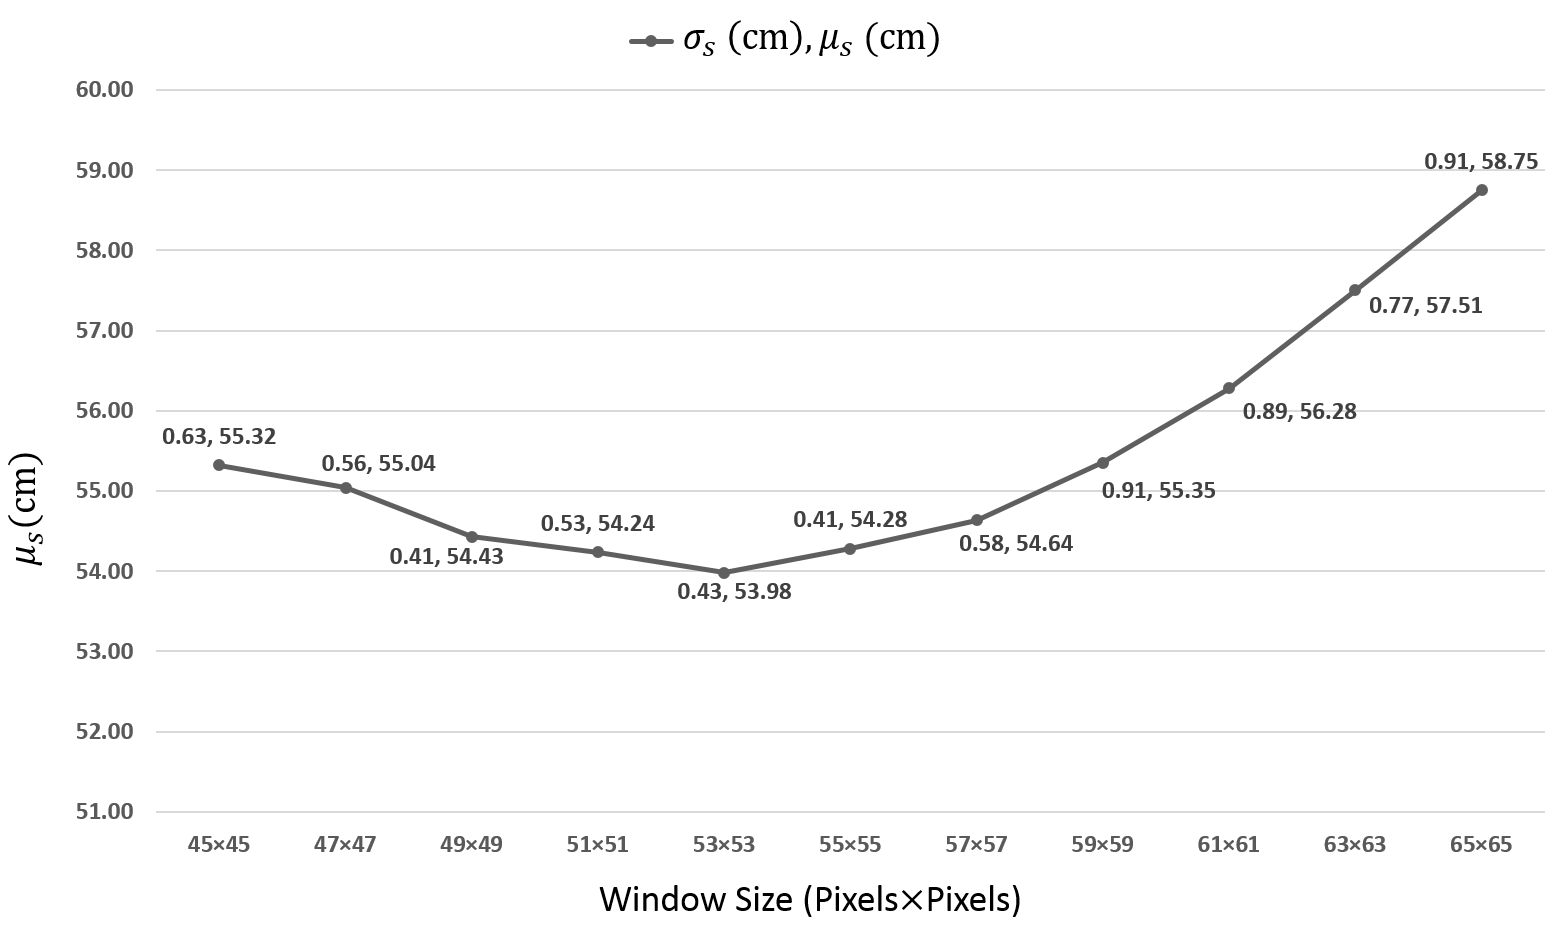
\includegraphics[width=\textwidth]{Figures/Results/SSD_Res.png}
    \caption{Effect of the ensemble window size on the SSD values.}
    \label{fig:swindow}
\end{figure}

The graphical representation in Figure \ref{fig:swindow} shows that when the window size is increased beyond 57$\times$57, the SSD values increase sharply whereas, between the windows 53$\times$53 and 57$\times$57, the values are mostly similar. This could be attributed by the fact that, in mountainous terrains, elevation, and not distance, plays a critical role in controlling the snow accumulation \citep{Liu2017, Singh2014, Singh2017, Thakur2012}. The varying topographical conditions prominently visible in Figure \ref{fig:field} also ascertain that for larger window sizes, the snow depth variability could increase if a nearby mountain also lies within the neighbourhood window. So, considering these aspects, the ensemble window size of 57$\times$57 is selected which results in $\mu_s \approx$ 54.64 cm with $\sigma_s \approx$ 0.58 cm as discussed in the scaling parameter sensitivity analysis.

\subsubsection{DEM and LIA Error Analysis}
\label{sssec:error}

During the field visit (section \ref{sssec:field}), several DGPS points which had been acquired are used to check the
accuracy of the ALOS PALSAR DEM (Fig \ref{fig:overview}). In essence, the observed errors are then used to analyse the change in the LIA (Eq. \eqref{eq:sa}) induced by the corrected DEM (the erroneous DEM pixels are replaced by the respective DGPS measurements). 

The DEM errors calculated using the Dhundi and Kothi DGPS readings are displayed in Figure \ref{subfig:dem_error} and the subsequent LIA differences (computed from the corrected and original DEMs) for these points are shown in Figure \ref{subfig:lia_error}. As seen from these graphs, the absolute elevation errors range from 0.08 m to 16.30 m in the Dhundi region, whereas these vary from 0.19 m to 25.32 m in the Kothi area. Accordingly, the RMSE values for the elevation errors are approximately 6.71 m and 8.8 m respectively.

\begin{figure}[!ht]
    \centering
    \begin{subfigure}[t]{\textwidth}
        \raisebox{-\height}{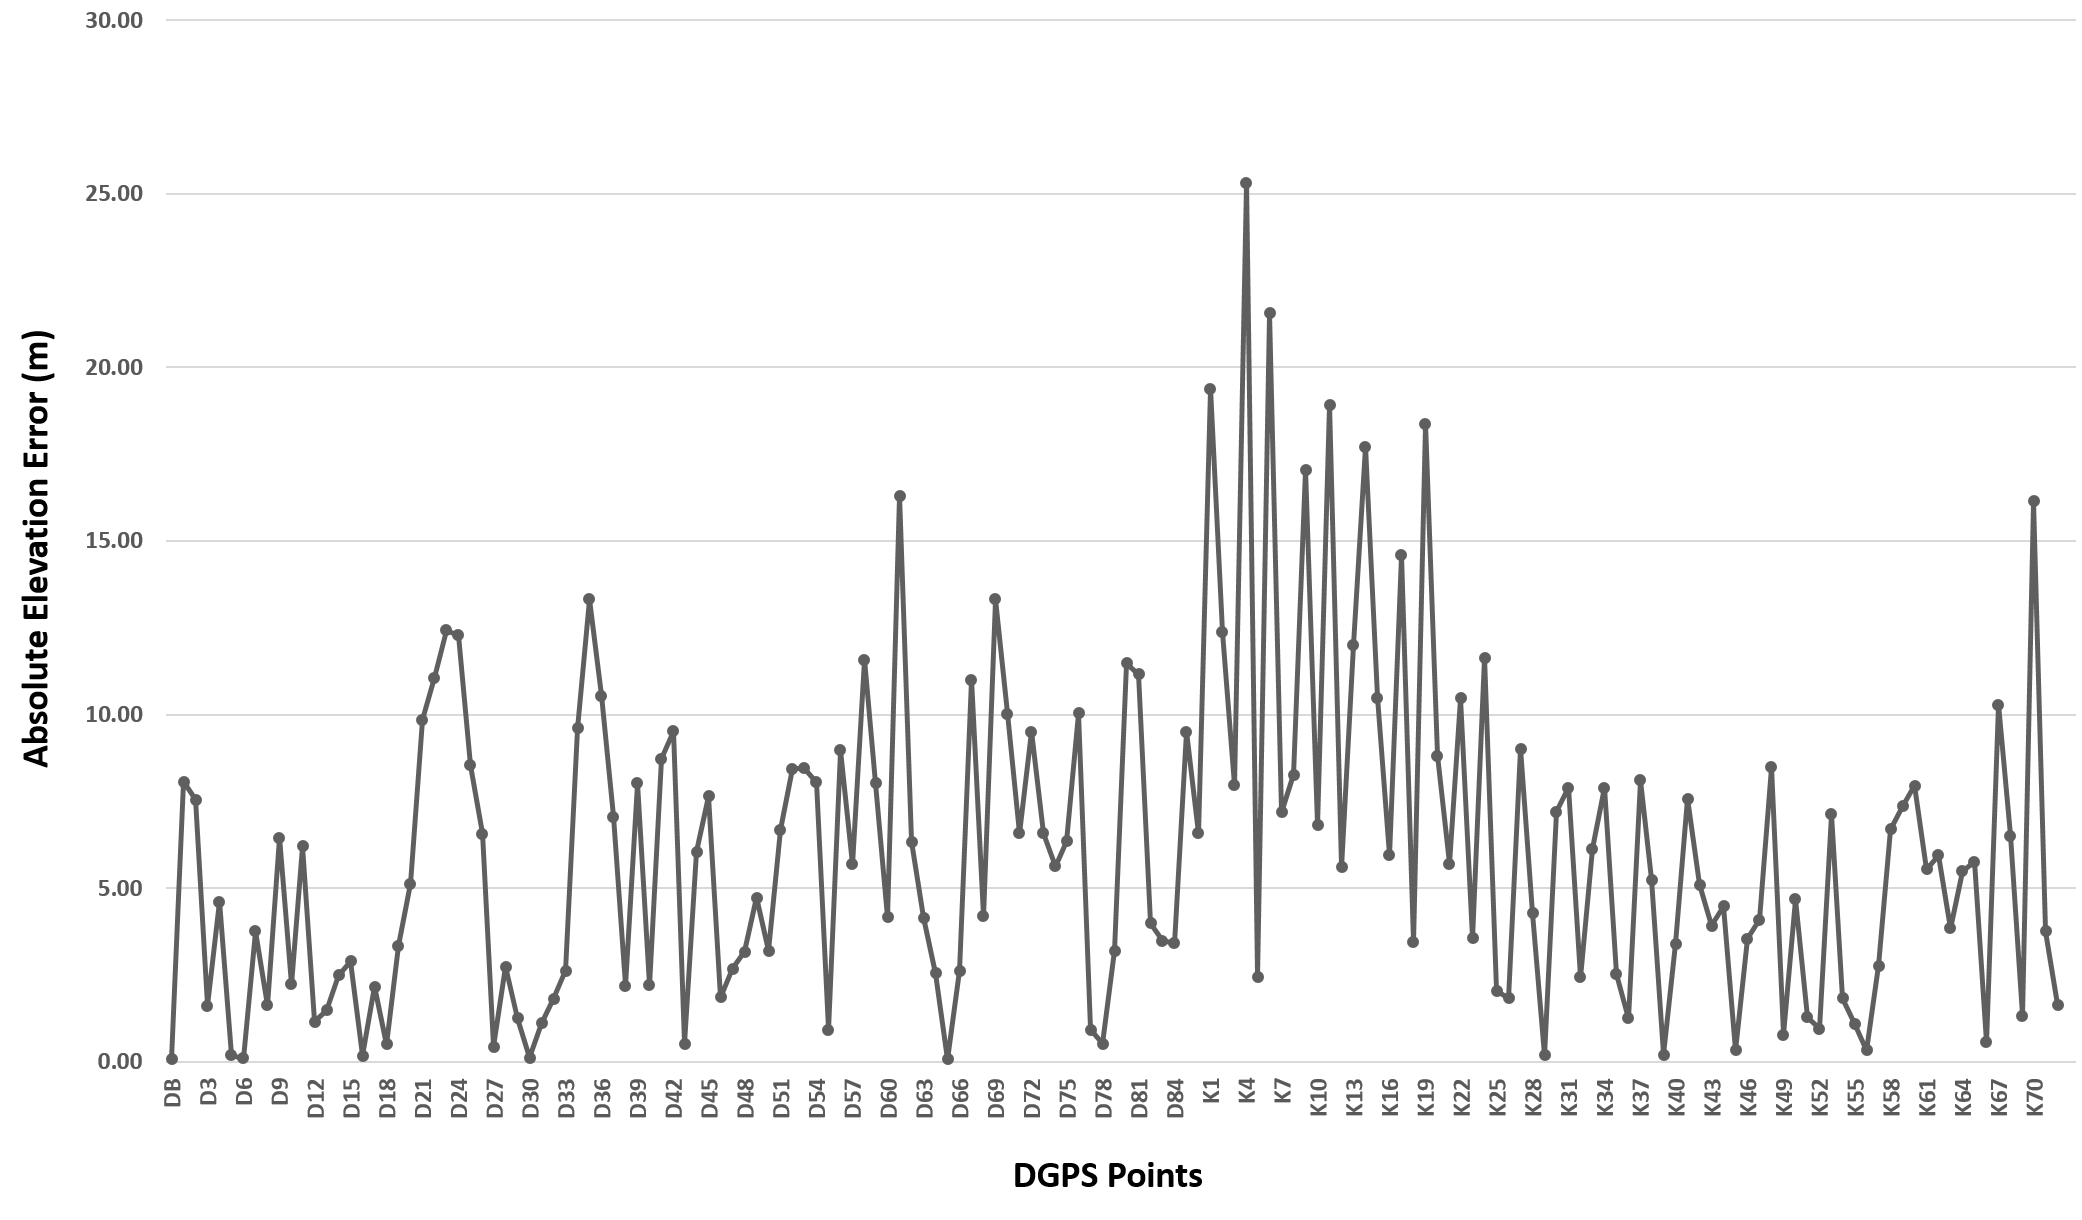
\includegraphics[width=\textwidth]{Figures/Results/DEM_Error.png}}
        \caption{}
        \label{subfig:dem_error}
    \end{subfigure}
    %%%%%%%%%%%%%%%%%%%%%%%%%%%%%%%%%%%second row
    \begin{subfigure}[t]{\textwidth}
        \raisebox{-\height}{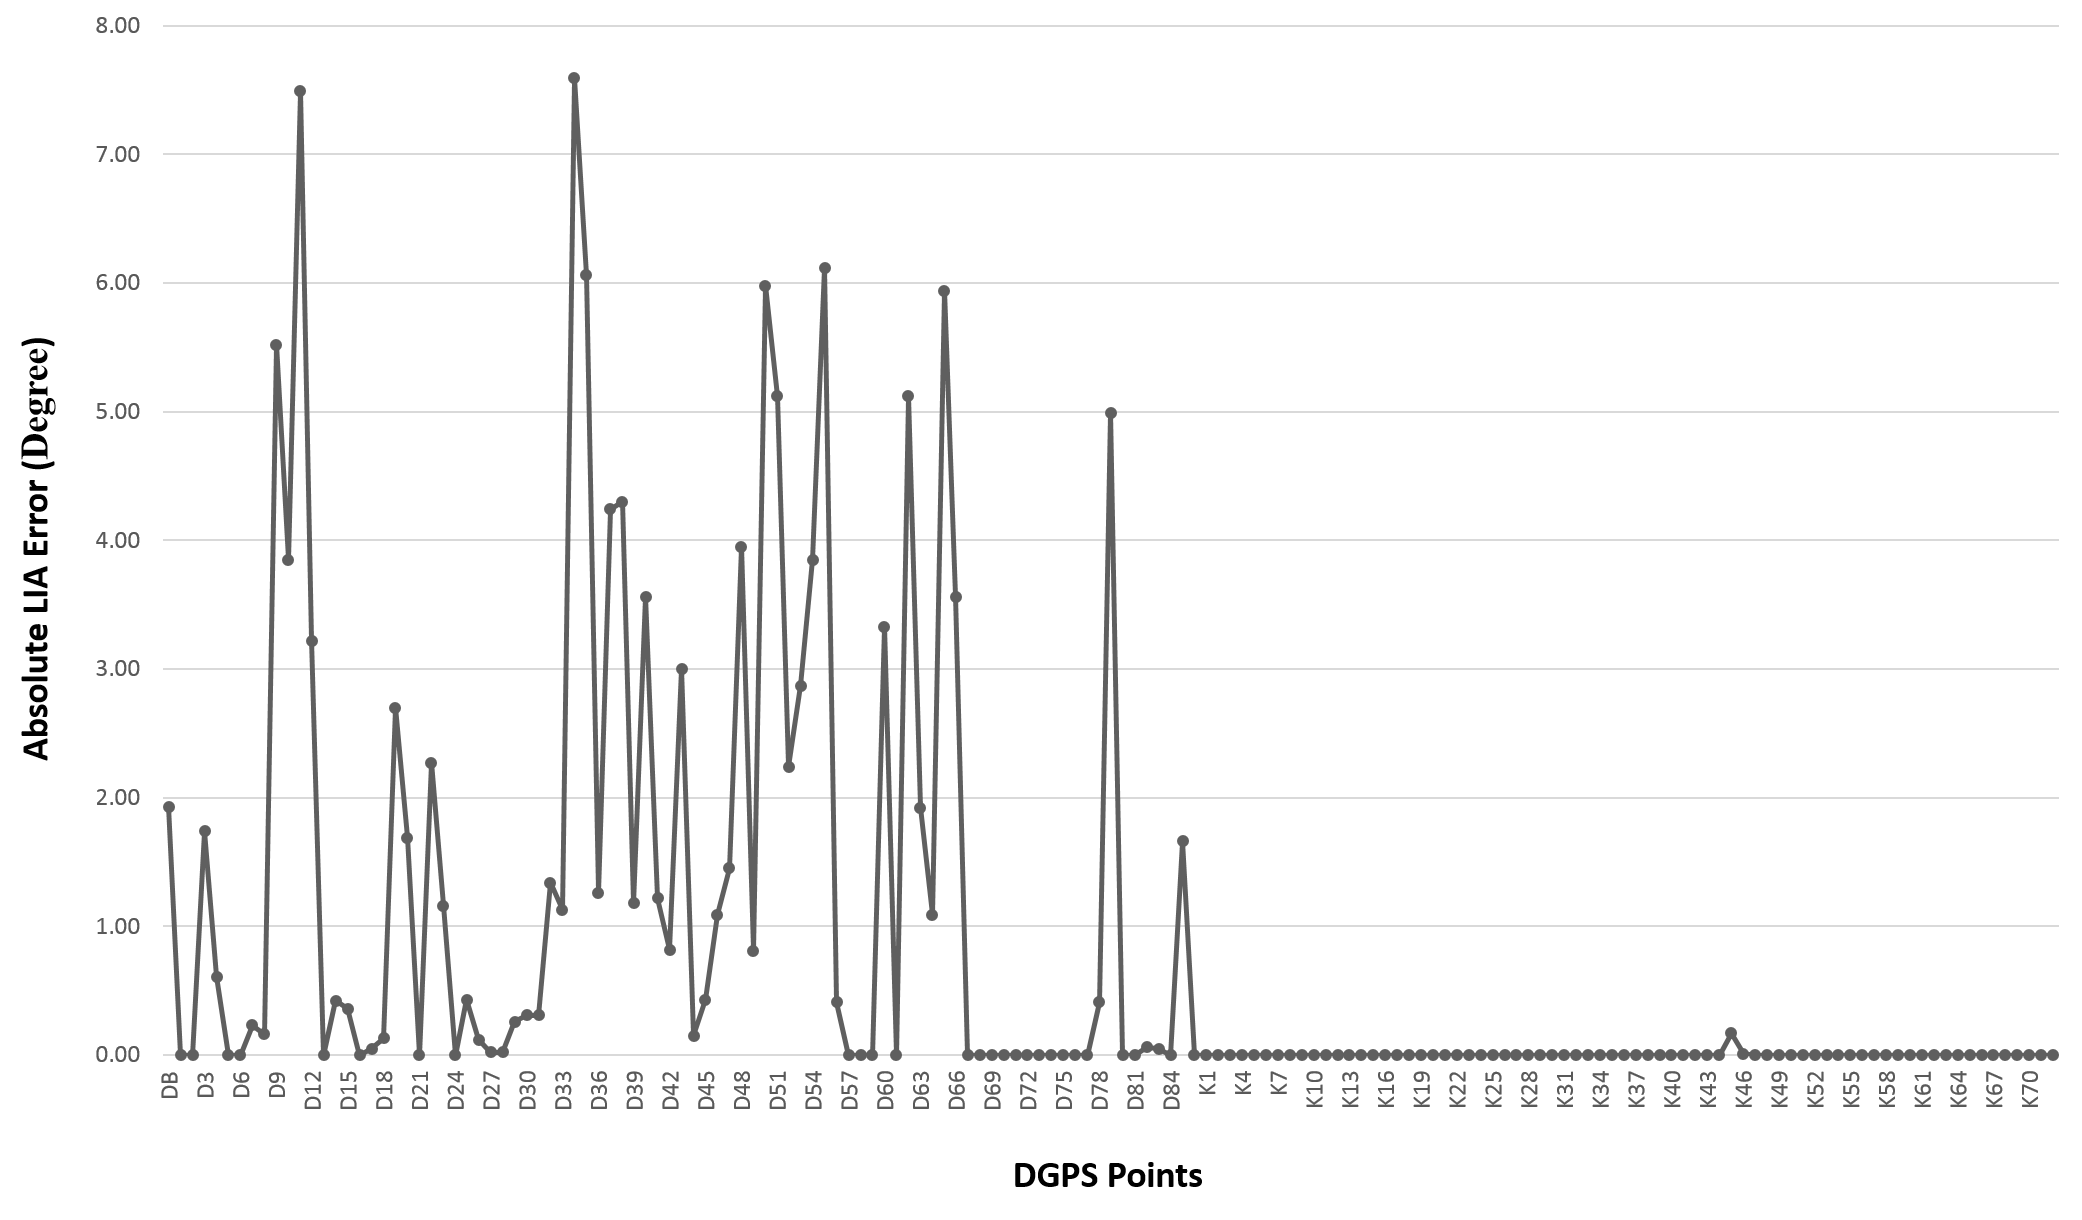
\includegraphics[width=\textwidth]{Figures/Results/LIA_Error.png}}
        \caption{}
        \label{subfig:lia_error}
    \end{subfigure}
    \caption{\subref{subfig:dem_error} Absolute DEM errors obtained by comparing ALOS PALSAR DEM and the DGPS measurements and \subref{subfig:lia_error} observed absolute LIA errors. Here, DB is the Dhundi base station point, D1-D86 are acquired in the Dhundi region, and K1-K72 are measured in the Kothi area using the DGPS. All these values are rounded to 2 decimal places.}
    \label{fig:error}
\end{figure}

In addition, the LIA errors vary from 0$^\circ$ to 7.59$^\circ$ (Dhundi) and 0$^\circ$ to 0.17$^\circ$ (Kothi) in these areas with the corresponding RMSE being nearly 2.54$^\circ$ and 0.02$^\circ$. Since only the pixels corresponding to the ground surveyed points are replaced with the modified LIA, so while calculating the slope, the errors may not be large because the neighbouring pixels could still have associated LIA errors which remain uncorrected. Thus, when the LIA errors are rounded to 2 decimal places as in Fig \ref{subfig:lia_error}, several values are exactly 0$^\circ$. Furthermore, as the LIA is dependent on the slope values (Eq. \eqref{eq:sa}), the DEM errors do not significantly influence the LIA. Also, in the vertical wavenumber calculation used in the SSD estimation given by Eq. \eqref{seq:vn}, the sine ($\sin$) of the LIA is considered. So, the minute changes in the LIA do not strongly affect the SSD estimates which are obtained after applying sufficient ensemble averaging operation (section \ref{sec:method}). Evidently, the LIA only changes by about 1.9$^\circ$ near the Dhundi base station and hence, the SSD results are not exhibiting any sizeable impact from the associated DEM errors.

Therefore, the sensitivity analysis concerning the DEM errors and its propagation highlights that the subsequent LIA errors are not directly governed by the changes in the elevation values, rather the slopes in $x$ and $y$ directions (section \ref{sssec:sa}) act as the primary error sources. Also, the ALOS PALSAR DEM is sufficiently accurate even in the complex terrains and hence, its usage in the LIA computation is justified.
\FloatBarrier
\subsection{Comparative Analysis of the Estimates}
\label{ssec:snow}

In order to visually observe the spatial patterns, the SSD maps for all the datasets were prepared but only the January 8, 2016 map is shown in Figure \ref{fig:ssd_map}. The respective SSWE maps are not provided as these have been computed by multiplying the constant standing snow densities (Table \ref{table:ssd_data}) to the SSD values. Therefore, they have similar spatial characteristics like those of the snow depth maps.

\afterpage{\FloatBarrier}
\begin{figure}[htb]
    \centering
    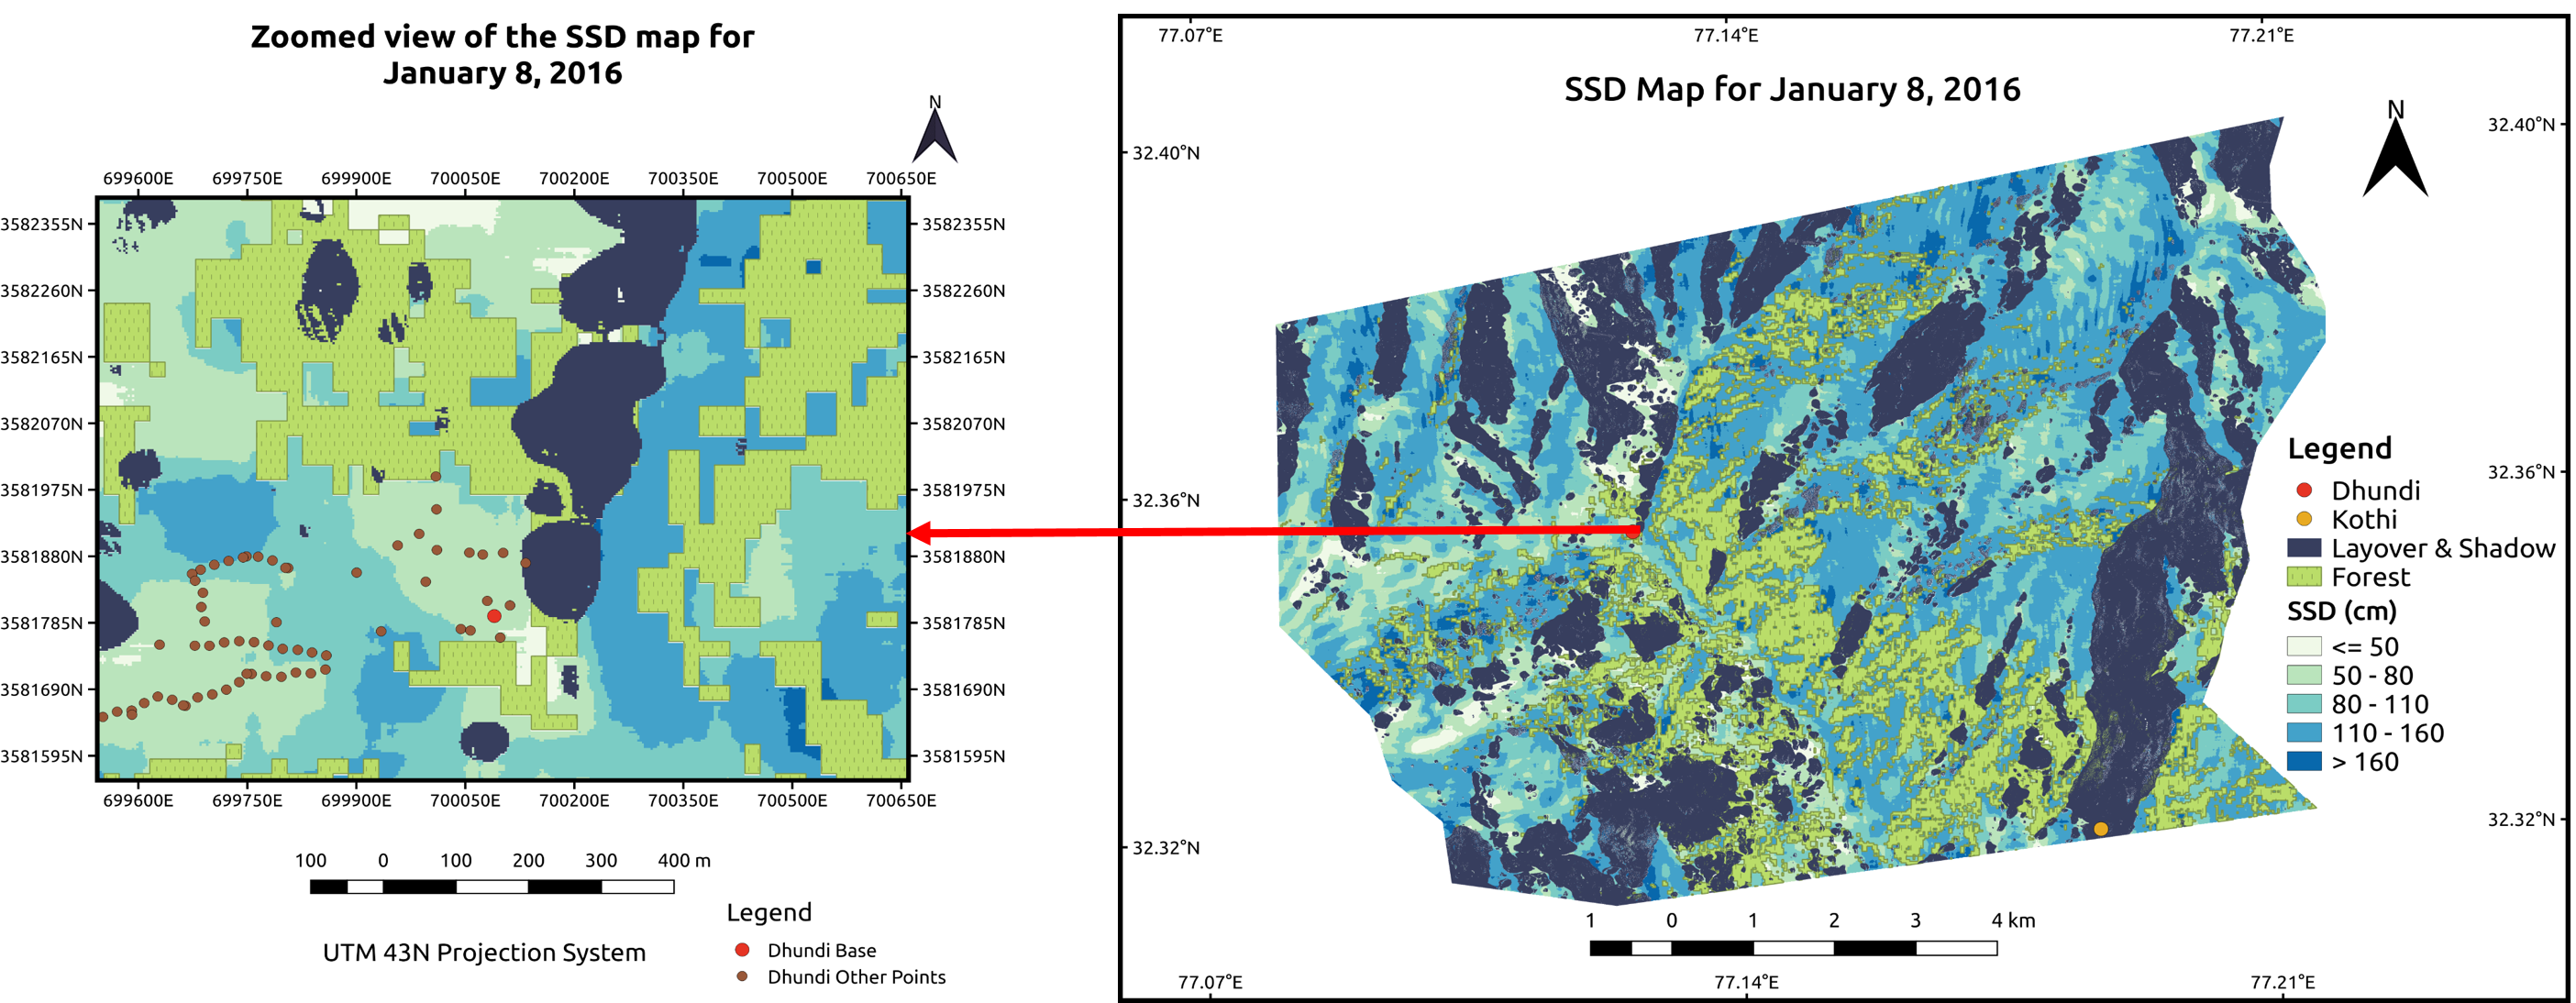
\includegraphics[width=\textwidth]{Figures/Results/SSD.png}
    \caption{Zoomed view of the SSD map for January 8, 2016. The ground points surveyed (section \ref{sssec:field}) are shown wherein the closely spaced points have been acquired using the DGPS kinematic mode and fall on the nearby roads in the Dhundi region. The other points including the Dhundi base are measured using the static mode. Since the Kothi area falls in the layover and shadow zone, it is excluded from the zoomed view analysis.}
    \label{fig:ssd_map}
\end{figure}

The complete analysis of all the datasets are provided in Table \ref{table:ssd_results} which shows that for the Dhundi site, the improved model displays sufficiently high overall SSD accuracy with coefficient of determination ($R^2$) $\approx$ 0.97, Mean Absolute Error (MAE) $\approx$ 1.56 cm, and Root Mean Square Error (RMSE) $\approx$ 1.89 cm. The corresponding SSWE estimates have $R^2 \approx$ 0.78, MAE $\approx$ 4.84 mm, and RMSE $\approx$ 6.01 mm. This reduction in the $R^2$ for the SSWEs indicate that even small errors present in the SSD estimates can greatly influence the estimated SSWEs. In Table \ref{table:ssd_results}, $\epsilon_s$ and $\epsilon_{ss}$ are the SSD and SSWE errors respectively with $\mu_s$, $\mu_{ss}$, $\sigma_s$, and $\sigma_{ss}$ having same meanings as in section \ref{sssec:scale}.

\begin{table}[!ht]
\centering
\caption{Accuracy assessment of the SSD and SSWE estimates in the Dhundi region. Here, the negative and positive errors represent overestimation and underestimation respectively. The date is represented in DD/MM/YYYY format and all the values are rounded to 2 decimal places.}
\label{table:ssd_results}
\begin{tabular}{c c c c c c c}
\hline
\textbf{Date}   & \boldmath{$\mu_s$} \textbf{(cm)} & \boldmath{$\sigma_s$} \textbf{(cm)} & \boldmath{$\epsilon_s$} \textbf{(cm)}    & \boldmath{$\mu_{ss}$} \textbf{(mm)} & \boldmath{$\sigma_{ss}$} \textbf{(mm)} & \boldmath{$\epsilon_{ss}$} \textbf{(mm)}  \\ \hline
29/12/2015  & 38.05 & 0.64  & -1.35 & 145.34    & 2.44  & -5.15 \\ 
08/01/2016  & 54.64 & 0.58  & 0.26  & 172.10    & 1.82  & 0.84  \\ 
09/01/2016  & 53.55 & 0.30  & 2.45  & 162.81    & 0.92  & 7.43  \\ 
19/01/2016  & 43.08 & 0.17  & -0.28 & 149.50    & 0.60  & -0.98 \\ 
20/01/2016  & 39.57 & 0.36  & 3.23  & 133.74    & 1.20  & 10.92 \\
30/01/2016  & 71.77 & 0.27  & -1.77 & 150.72    & 0.57  & -3.72 \\ \hline
\end{tabular}
\end{table}

Moreover, the large variations in the SSD and SSWE for the complete region (Fig \ref{fig:ssd_map}) highlight the extreme topographical conditions present in the study area. These variations can be confirmed from the ground survey (section \ref{sssec:field}) where the points (shown in Figure \ref{fig:ssd_map}) had been acquired by considering the terrain undulations. Also, the aspect, slope, and elevation significantly influence the SSD estimates, the details of which have been discussed in the previous section.

Apart from this, it was observed that these estimates are lower in the Dhundi base station area as compared to the surrounding regions. This phenomenon can be attributed to the presence of the human settlements (Figure \ref{subfig:base}) near the base point and are expected to have less snow accumulation than the natural surroundings. Moreover, the effect of multiple or double bounce scattering (Z4) near the Dhundi base is prominent even during the winter (Figure \ref{subfig:wishart_jan}). So, this could effectively reduce the volume and surface coherences (section \ref{ssec:ssd}) thereby explaining this observation.

\section{Conclusion and Future Scope}
\label{sec:conc}

The primary focus of this research lies in estimating the SSD using the improved hybrid DEM differencing and coherence amplitude inversion algorithm based on the single-baseline Pol-InSAR technique (section \ref{ssec:ssd}). A time series analysis of the SSD estimates involving six TSX/TDX datasets acquired between December 2015 and January 2016 have been performed. Accordingly, the corresponding SSWEs are obtained by multiplying fixed standing snow densities for each epoch.

Due to the complex hydrometeorological and topographical conditions of the study area (section \ref{sssec:geo}), significant uncertainty sources are present. These include the forests, boulders, highly rough surfaces, and human settlements (Figure \ref{fig:field}) which substantially reduce the surface and volume scattering coherences required to estimate the snow depths with adequate accuracy (section \ref{ssec:vus}). Moreover, the limited ground-truth data availability has always been a major challenge from the onset of this work (section \ref{ssec:data}). Apart from this, the SAR data are affected by layover, shadowing and foreshortening in mountainous terrains and hence, these errors are inherently propagated through the subsequent processing steps. Furthermore, the Pol-InSAR model involves several user-defined parameters which have to be optimised (section \ref{sec:method}). In short, these are the main concerns involved in this work which are addressed by means of identifying the potential uncertainty sources ($H/{\alpha}$ decomposition and Wishart classification) and performing appropriate sensitivity analysis (section \ref{sssec:sa}).

Thus, the novelty of this research lies in suitably modifying and ultimately improving the hybrid Pol-InSAR model (section \ref{ssec:ssd}) to estimate the SSD which is new in the context of cryospheric studies. Although there was only a single spatial validation point (Dhundi), the SSD estimates show high accuracy when the temporal trends are considered. Intriguingly, only one of the free parameters, $\eta^\prime$, needed to be tweaked for the time series analysis. Therefore, the results suggest that the SSD inversion model works sufficiently well under the complex hydrometeorological situations.

As part of future work, it is recommended to use the multi-baseline Pol-InSAR technique \citep{Cloude2010} wherein $k_z$ can be simulated (instead of scaling by $\eta^\prime$) after an appropriate accuracy assessment \citep{Kumar2017}. Similarly, the effect of different window shapes (square or rectangular) and sizes can be considered for the ensemble averaging operation. This sort of sensitivity analysis will help in deciding optimal window structures separately for each model. Moreover, it is recommended to apply scattering mechanism based masks in conjunction with snow masks prepared from the high resolution optical datasets such as those provided by Sentinel-2 \citep{Zhu2015}. In addition, the prior classification of the dry and wet snow including the preparation of snow cover maps \citep{Leinss2018, Thakur2012, Zhu2015} as necessary preprocessing steps will certainly improve the uncertainty assessment process.

Also, the use of the newer multi-temporal high resolution L-band datasets acquired by the upcoming SAR missions \citep{Tridon2018, Rosen2017} is recommended to further verify and validate these models. Moreover, radar altimeters such as the Ka-band InSAR altimeter could potentially improve the SD and SWE estimates, and could also be used for operational snow depth monitoring on a large-scale \citep{Hensley2016, Kim2018, Moller2011, Speziali2018}.

In this work, only six datasets were used for analysis. Preferably, if a full scale time series analysis involving several epochs and multiple validation sites is performed, then the robustness of the SSD retrieval model can be even appropriately verified. Furthermore, Pol-InSAR coherency optimisation can be carried out to suitably adjust the scattering phase centres \citep{Cloude2005, Cloude2010}. Moreover, the snow densities need to be computed gridwise (or if possible, pixelwise) by using hydrological modelling approaches \citep{Bartelt2002, Liang1994}. These can also be estimated from the PolSAR based techniques which are in practice \citep{Singh2017, Thakur2012}. Finally, necessary statistical hypothesis testing is required to suitably quantify the uncertainties associated with the SSD and SSWE estimates.

\section*{Acknowledgements}
This research work was carried out as part of the ISRO EOAM mountain ecosystem, TANDEM-X AO and ALOS-RA4 project (EOAM-ME (WRD)) on the Himalayan glaciers. Also, this work was conducted within the IIRS, ISRO and University of Twente, Faculty ITC joint education programme (JEP) framework. The authors are grateful to IIRS, ISRO, University of Twente, Faculty ITC along with SASE, DRDO and the entire opensource community for providing the necessary means to conduct this study.  

\section*{References}
\footnotesize{\bibliography{refs}}

\end{document}